\iffalse \bibliography{MGymrekRefs.bib} \fi

\chapter{Abundant contribution of short tandem repeats to gene expression variation in humans}
\label{chap:estr}
\hzline

Most of this chapter was first published as:

\begin{itemize}
\item[] \textbf{Gymrek M}, Willems TF, Guilmatre A, Zeng H, Markus B, Georgiev S, Daly MJ, Price AL, Pritchard JK, Sharp AJ, Erlich Y. Abundant contribution of short tandem repeats to gene expression variation in humans. \emph{Nature Genetics}. (2015).
\end{itemize}

\hzline

\textbf{Abstract:} The contribution of repetitive elements to quantitative human traits is largely unknown. Here, we report a genome-wide survey of the contribution of Short Tandem Repeats (STRs), one of the most polymorphic and abundant repeat classes, to gene expression in humans. Our survey identified 2,060 significant expression STRs (eSTRs). These eSTRs were replicable in orthogonal populations and expression assays. We used variance partitioning to disentangle the contribution of eSTRs from linked SNPs and indels and found that eSTRs contribute 10\%-15\% of the cis-heritability mediated by all common variants. Further functional genomic analyses showed that eSTRs are enriched in conserved regions, co-localize with regulatory elements, and can modulate certain histone modifications. By analyzing known GWAS hits and searching for new associations in 1,685 deeply-phenotyped whole-genomes, we found that eSTRs are enriched in various clinically-relevant conditions. These results highlight the contribution of short tandem repeats to the genetic architecture of quantitative human traits.

\section{Introduction}
In recent years, there has been tremendous progress in identifying genetic variants that affect expression of nearby genes, termed cis expression quantitative trait loci (cis-eQTLs). Multiple studies have shown that disease-associated variants often overlap cis-eQTLs in the affected tissue \cite{MoffattKabeschLiangEtAl2007,BarrettHansoulNicolaeEtAl2008,ArdlieDelucaSegreEtAl2015}. These observations suggest that understanding the genetic architecture of the transcriptome may provide insights into the cellular-level mediators underlying complex traits \cite{NicaMontgomeryDimasEtAl2010,NicolaeGamazonZhangEtAl2010,WardKellis2012}. So far, eQTL-mapping studies have mainly focused on SNPs and to a lesser extent on bi-allelic indels and CNVs as determinants of gene expression \cite{StrangerForrestDunningEtAl2007,GrundbergSmallHedmanEtAl2012,LappalainenSammethFriedlanderEtAl2013}. However, these variants do not account for all of the heritability of gene expression attributable to cis-regulatory elements as measured by twin studies, leaving on average about 20-30\% unexplained \cite{GrundbergSmallHedmanEtAl2012,WrightSullivanBrooksEtAl2014}.  It has been speculated that such heritability gaps could indicate the involvement of repetitive elements that are not well tagged by common SNPs \cite{ManolioCollinsCoxEtAl2009,PressCarlsonQueitsch2014}. 

To augment the repertoire of eQTL classes, we focused on Short Tandem Repeats (STRs), one of the most polymorphic and abundant types of repetitive elements in the human genome \cite{Ellegren2004,GemayelVincesLegendreEtAl2010}. These loci consist of periodic DNA motifs of 2-6bp spanning a median length of around 25bp. There are about 700,000 STR loci covering almost 1\% of the human genome. Their repetitive structure induces DNA-polymerase slippage events that add or delete repeat units, creating mutation rates that are orders of magnitude higher than those of most other variant types \cite{WeberWong1993,Ellegren2004}. Over 40 Mendelian disorders, such as Huntington's Disease, are attributed to STR mutations, most of which are caused by large expansions of trinucleotide coding repeats \cite{Mirkin2007}. 

Several properties of STRs suggest they may play a regulatory role. In vitro studies have shown that STR variations can modulate the binding of transcription factors \cite{ContenteDittmerKochEtAl2002,MartinMakepeaceHillEtAl2005}, change the distance between promoter elements \cite{WillemsPaulHeideEtAl1990,YogevRosengartenWatson-McKownEtAl1991}, alter splicing efficiency \cite{HefferonGromanYurkEtAl2004,HuiHungHeinerEtAl2005}, and induce irregular DNA structures that may modulate transcription \cite{RothenburgKoch-NolteRichEtAl2001}. In vivo experiments have reported specific examples of STR variations that control gene expression across a wide range of taxa, including Haemophilus influenza \cite{WeiserLoveMoxon1989}, Saccharomyces cerevisiae \cite{VincesLegendreCaldaraEtAl2009}, Arabidopsis thaliana \cite{SureshkumarTodescoSchneebergerEtAl2009}, and vole \cite{HammockYoung2005}. Recent studies reported that dinucleotide repeats are a hallmark of enhancers in Drosophila and are enriched in predicted enhancers in humans \cite{Yanez-CunaArnoldStampfelEtAl2014}. Human promoters also disproportionately harbor STRs \cite{SawayaBagshawBuschiazzoEtAl2013} and the presence of STRs in promoters or transcribed regions greatly increases the divergence of gene expression profiles across great apes \cite{SonayCarvalhoRobinsonEtAl2015}, suggesting that STRs play a key role in the evolution of expression. Several candidate-gene studies in human indeed reported that STR variations modulate gene expression \cite{GebhardtZankerBrandt1999,ShimajiriArimaTanimotoEtAl1999,WarpehaXuLiuEtAl1999,ContenteDittmerKochEtAl2002,RockmanWray2002} and alternative splicing \cite{HuiStanglLaneEtAl2003,HefferonGromanYurkEtAl2004,SathasivamNeuederGipsonEtAl2013}. In one example, a recent study found that the underlying mechanism behind a GWAS signal for Ewing Sarcoma is a sequence variant in an AAGG repeat that increases the binding of the EWSR1-FLI1 oncoprotein resulting in EGF2 overexpression \cite{GrunewaldBernardGilardi-HebenstreitEtAl2015}. Despite these accumulating lines of evidence, there has been no systematic evaluation of the contribution of STRs to gene expression in humans. 

To this end, we conducted a genome-wide analysis of STRs that affect expression of nearby genes, termed expression STRs (eSTRs), in lymphoblastoid cell lines (LCLs), a central ex-vivo model for eQTL studies. Next, we used a multitude of statistical genetic and functional genomics analyses to show that hundreds of these eSTRs are predicted to be functional. Finally, we tested the involvement of eSTRs in clinically relevant phenotypes.

\section{Results}
\subsection{Initial genome-wide discovery of eSTRs}
The initial genome-wide discovery of potential eSTRs relied on finding associations between STR length and expression of nearby genes. We focused on 311 European individuals whose LCL expression profiles were measured using RNA-sequencing by the gEUVADIS \cite{LappalainenSammethFriedlanderEtAl2013} project and whose whole genomes were sequenced by the 1000 Genomes Project \cite{AbecasisAltshulerAutonEtAl2010}. The STR genotypes were obtained in our previous study \cite{WillemsGymrekHighnamEtAl2014} in which we created a catalog of STR variation as part of the 1000 Genomes Project using lobSTR, a specialized algorithm for profiling STR variations from high throughput sequencing data \cite{GymrekGolanRossetEtAl2012}. Briefly, lobSTR identifies reads with repetitive sequences that are flanked by non-repetitive segments. It then aligns the non-repetitive regions to the genome using the STR motif to narrow the search, thereby overcoming the gapped alignment problem and conferring alignment specificity. Finally, lobSTR aggregates aligned reads and employs a model of STR-specific sequencing errors to report the maximum likelihood genotype at each locus. lobSTR recovered most ($r^2$=0.71) of the variation in STR locus lengths in the 1000 Genomes datasets based on large-scale validation using 5,000 STR genotype calls obtained by capillary electrophoresis, the gold standard for STR genotyping \cite{WillemsGymrekHighnamEtAl2014}. The majority of genotype errors were from dropout of one allele at heterozygote sites due to low sequencing coverage. We simulated the performance of STR associations using lobSTR calls compared to the capillary calls. This process showed that STR genotype errors reduce the power to detect eSTRs by 30-50\% but importantly do not create spurious associations (\textbf{Supplementary Note \ref{sec:estrsupnote}} and \textbf{Supplementary Fig. \ref{fig:estrsupfig1}}).

To detect eSTR associations, we regressed gene expression on STR dosage, defined as the sum of the two STR allele lengths in each individual. We opted to use this measure based on previous findings that reported a linear trend between STR length and gene expression \cite{GebhardtZankerBrandt1999,ShimajiriArimaTanimotoEtAl1999,ContenteDittmerKochEtAl2002} or disease phenotypes \cite{LaSpadaRolingHardingEtAl1992,DuyaoAmbroseMyersEtAl1993}. As covariates, we included sex, population structure, and other technical parameters (\textbf{Fig. \ref{fig:estrfig1}a} and \textbf{Supplementary Note \ref{sec:estrsupnote}}). We employed this process on 15,000 coding genes whose expression profiles were detected in the RNA-sequencing data. For each gene, we considered all polymorphic STR variations that passed our quality criteria (\textbf{Online Methods \ref{sec:estrolm}}) and were within 100kb of the transcription start and end sites of the gene transcripts as annotated by Ensembl \cite{FlicekAhmedAmodeEtAl2013}.  On average, 13 STR loci were tested for each gene (\textbf{Supplementary Fig. \ref{fig:estrsupfig2}}), yielding a total of 190,016 STR$\times$gene tests.  

\begin{figure}[h!]
\centering
\label{fig:estrfig1}
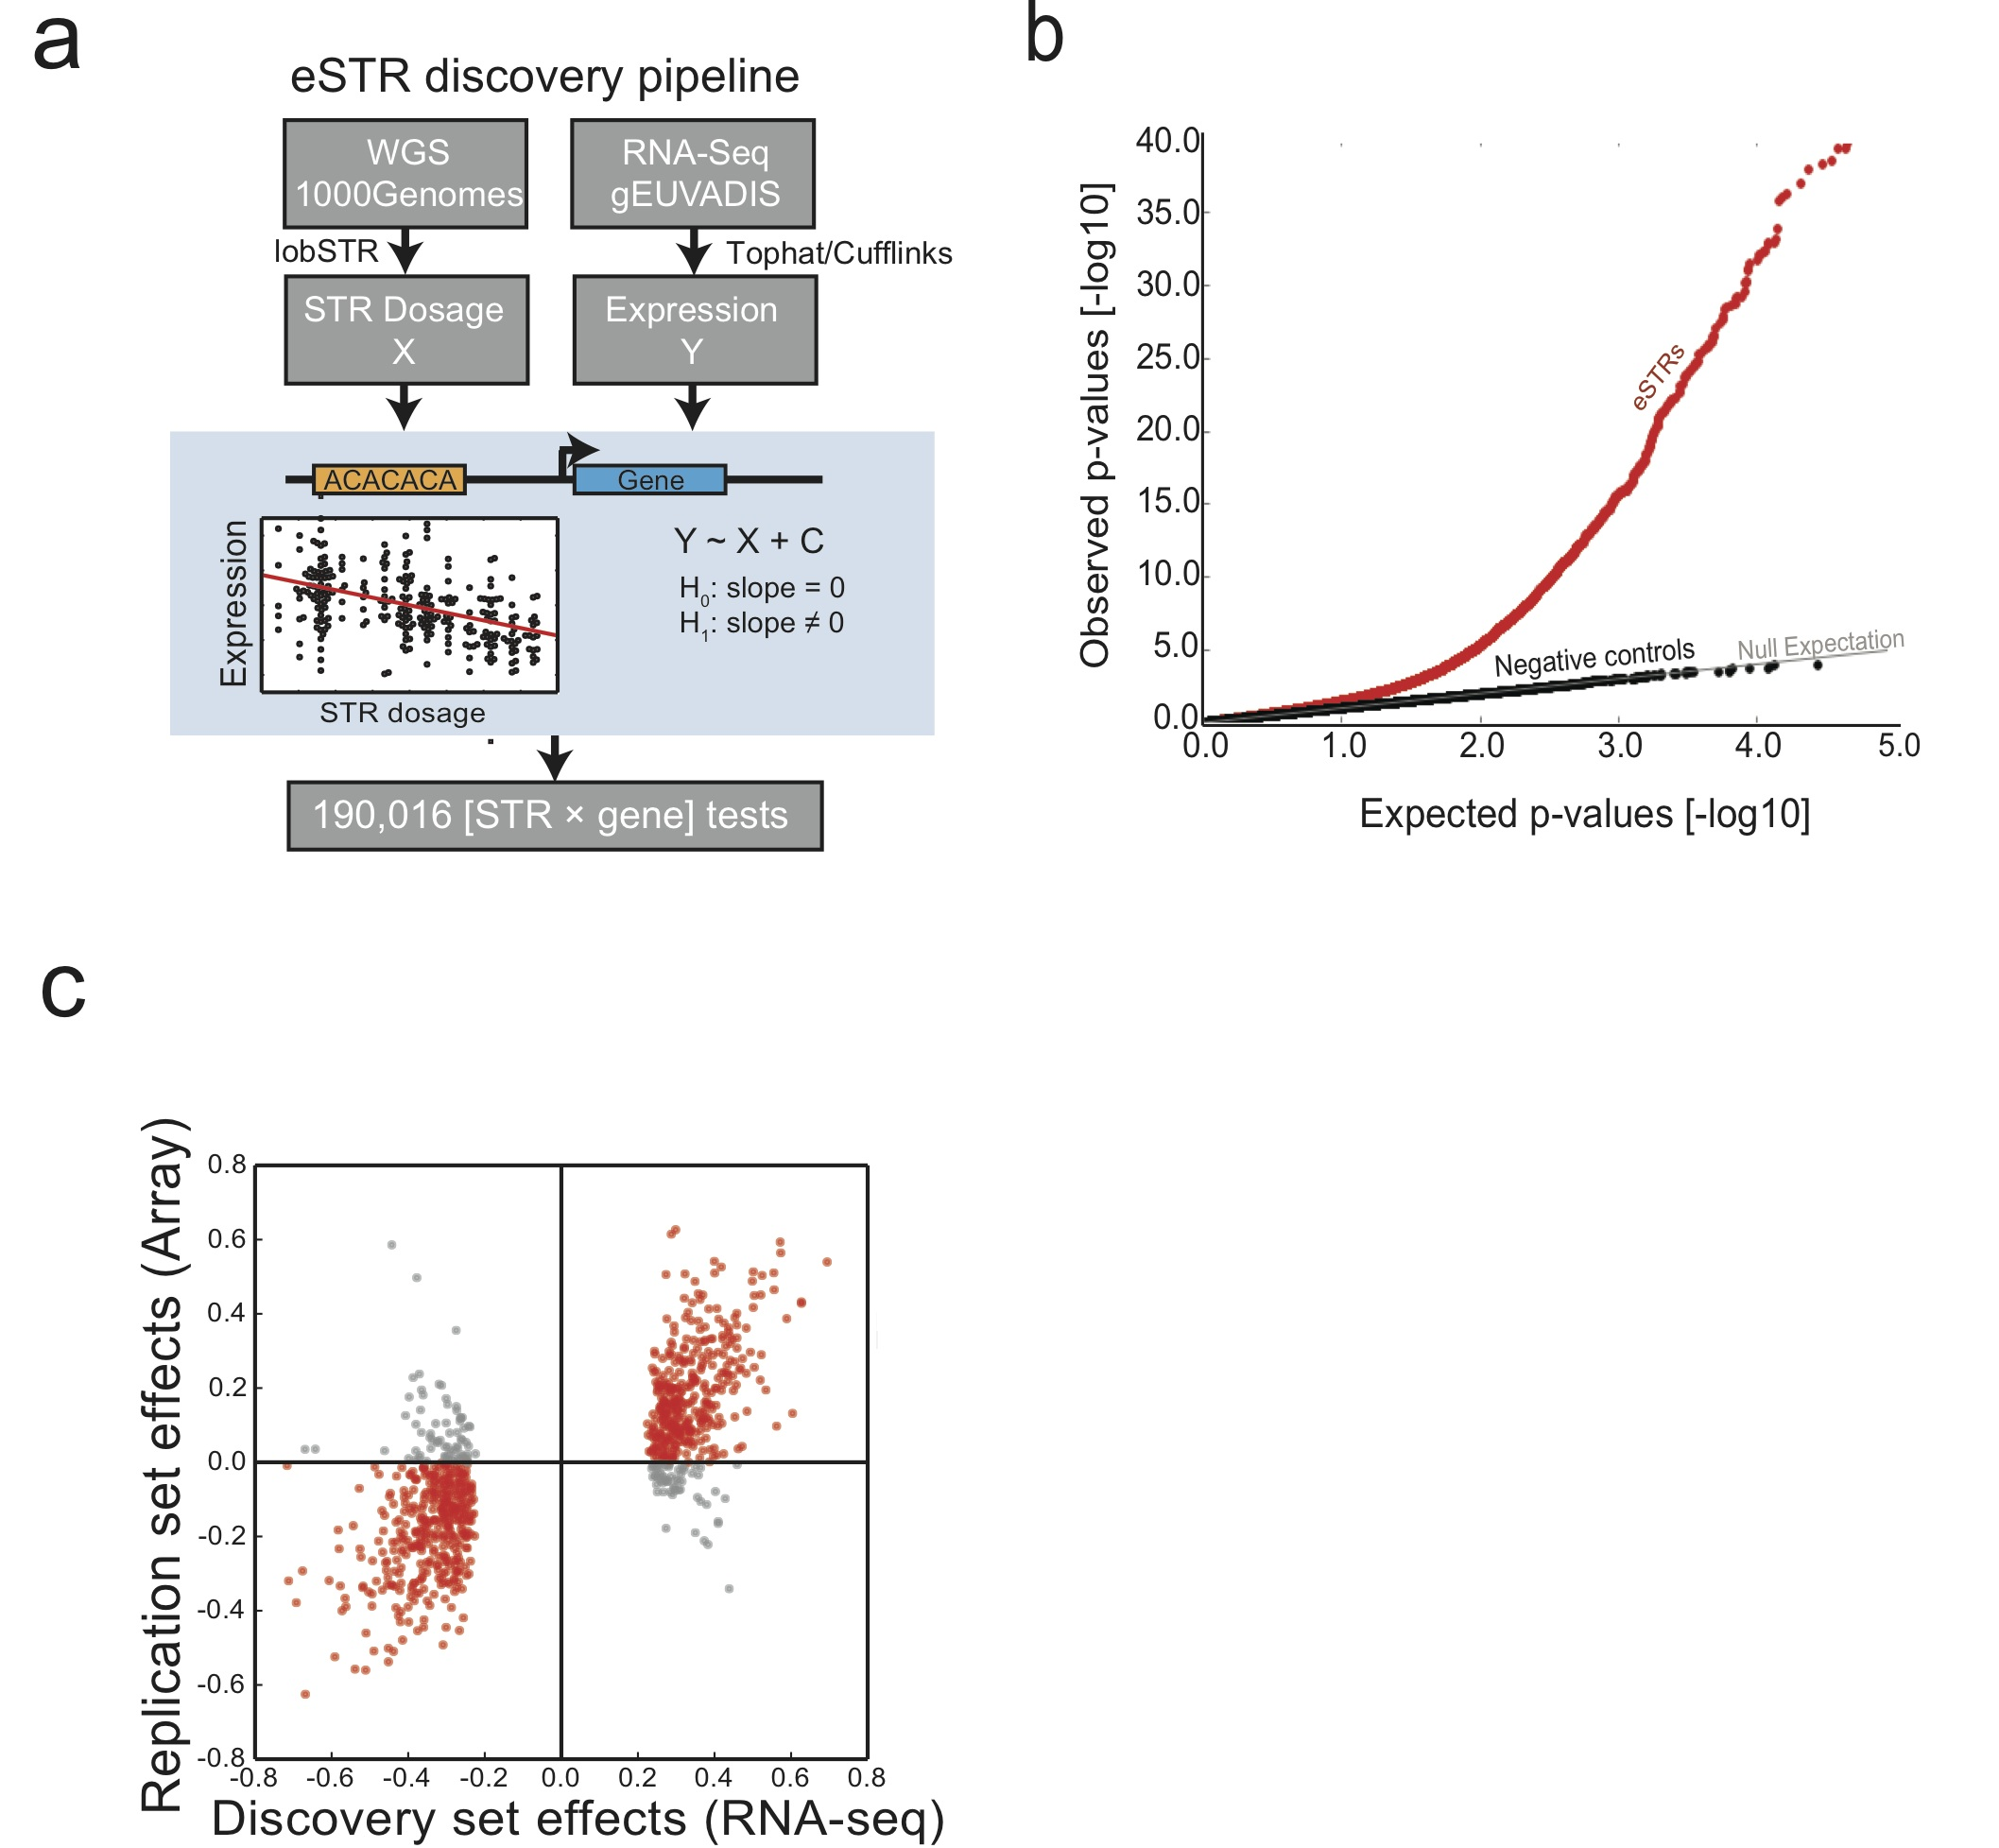
\includegraphics[width=0.9\textwidth]{Figures/Chapter4/Fig1}
\caption{\textbf{eSTR discovery and replication.} \textbf{(a)} eSTR discovery pipeline. An association test using linear regression was performed between STR dosage and expression level for every STR within 100kb of a gene \textbf{(b)} Quantile-quantile plot showing results of association tests. The gray line gives the expected p-value distribution under the null hypothesis of no association. Black dots give p-values for permuted controls. Red dots give the results of the observed association tests \textbf{(c)} Comparison of eSTR effect sizes as Pearson correlations in the discovery dataset vs. the replication dataset. Red points denote eSTRs whose directions of effect were concordant in both datasets and gray points denote eSTRs with discordant directions. }
\end{figure}

Our analysis identified 2,060 unique protein-coding genes with a significant eSTR (gene level FDR≤5\%) (\textbf{Fig. \ref{fig:estrfig1}b} and \textbf{Supplementary Data Set 1} (see \emph{Nature Genetics} website)). The majority of these were di- and tetra-nucleotide STRs (\textbf{Supplementary Tables \ref{tab:estrsuptab1}} and \textbf{\ref{tab:estrsuptab2}}). Only 13 eSTRs fall in coding exons, but eSTRs were nonetheless strongly enriched in 5'UTRs ($p=1.0 \times 10^{-8}$), 3'UTRs ($p=1.7\times10^{-9}$) and regions near genes ($p<10^{-28}$) compared to all STRs analyzed (\textbf{Supplementary Table \ref{tab:estrsuptab3}}). Overall, there was no bias in direction of effect (\textbf{Supplementary Table \ref{tab:estrsuptab4}}). We also repeated the association tests with two negative control conditions by regressing expression on (i) STR dosages permuted between samples and (ii) STR dosages from randomly chosen unlinked loci (\textbf{Fig. \ref{fig:estrfig1}b} and \textbf{Supplementary Fig. \ref{fig:estrsupfig3}}). Both negative controls produced uniform p-value distributions expected under the null hypothesis. This provides support for the absence of spurious associations due to inflation of the test statistic or the presence of uncorrected population structure. To assess the effect of low sequencing coverage on our results, we generated high coverage targeted sequencing of 2,472 promoter STRs and repeated the eSTR analysis (\textbf{Online Methods \ref{sec:estrolm}}). We found that association results were largely reproducible across datasets, with 80\% of tested eSTRs showing the same direction of effect ($p=9.9\times 10^{-12}$; $n=126$) (\textbf{Supplementary Note \ref{sec:estrsupnote}} and \textbf{Supplementary Fig. \ref{fig:estrsupfig4}}). Three previous studies described candidate gene studies of expression STRs and involved STRs that were tested in our framework \cite{GebhardtZankerBrandt1999,ShimajiriArimaTanimotoEtAl1999,ContenteDittmerKochEtAl2002}. Our genome-wide approach was able to replicate the association between \emph{PIG3} and the pentanucleotide STR in the 5'UTR of the gene and showed the same direction of effect. However, the other two candidate genes did not meet the multiple hypothesis p-value threshold (\textbf{Supplementary Table \ref{tab:estrsuptab5}}).

The initial discovery set of eSTRs was largely reproducible in an independent set of individuals using an orthogonal expression assay technology. We obtained an additional set of over 200 individuals whose genomes were also sequenced as part of the 1000 Genomes Project and whose LCL expression profiles were measured by Illumina expression array \cite{StrangerMontgomeryDimasEtAl2012}. These individuals belong to cohorts with African, Asian, European, and Mexican ancestry, enabling testing of the associations in a largely distinct set of populations. The Illumina expression array allowed us to test 882 eSTRs out of the 2,060 identified above. The association signals of 734 of the 882 (83\%) tested eSTRs showed the same direction of effect in both datasets (sign test $p=2.7 \times 10^{-94}$) and the effect sizes were strongly correlated ($R=0.73$, $p=1.4 \times 10^{-149}$) (\textbf{Fig. \ref{fig:estrfig1}c}), despite only moderate reproducibility of expression profiles across platforms (\textbf{Supplementary Note \ref{sec:estrsupnote}} and \textbf{Supplementary Fig. \ref{fig:estrsupfig5}}). For comparison, only 54\% of non-eSTRs showed the same direction of effect, close to the expected value of 50\% for null associations. Overall, these results show that eSTR association signals are robust and reproducible across populations and expression assay technologies. 

\subsection{Partitioning the contribution of eSTR and nearby variants}
An important question is whether eSTR association signals stem from causal STR loci or are merely due to tagging SNPs or other variants in linkage disequilibrium (LD). Previous results reported that the average STR-SNP LD is approximately half of the traditional SNP-SNP LD \cite{PayseurPlaceWeber2008,WillemsGymrekHighnamEtAl2014} but there are known examples of STRs tagging GWAS SNPs \cite{LaminaHaunCoassinEtAl2014}.

To address this question, we partitioned the relative contributions of eSTRs versus all common (MAF$\geq$1\%) bi-allelic SNPs, indels, and structural variants (SV) in the cis region of each gene using a linear mixed model (LMM) (\textbf{Fig. \ref{fig:estrfig2}a}). Multiple studies have used this approach to measure the total contribution of common variants to the heritability of quantitative traits and to partition the contribution of different classes of variants \cite{YangBenyaminMcEvoyEtAl2010,GusevLeeNealeEtAl2014}. Taking a similar approach, we included two types of effects for each gene: a random effect ($h_b^2$) that captures all common bi-allelic loci detected within 100kb of the gene and a fixed effect ($h_{STR}^2$) that captures the lead STR. To test whether other causal variants in the local region could inflate the estimate of the STR contribution, we simulated gene expression with one or two causal SNP eQTLs per gene while preserving the local haplotype structure. In this negative control scenario, the LMM correctly reported a median ($h_{STR}^2$)$/$($h_{cis}^2 $) $\approx 0$ across all conditions (\textbf{Supplementary Note \ref{sec:estrsupnote}} and \textbf{Supplementary Fig. \ref{fig:estrsupfig6}, \ref{fig:estrsupfig7}}), where $h_{cis}^2=h_b^2+h_{STR}^2$. This suggests that other causal variants in LD do not inflate the estimate of the relative contribution of STRs. However, simulations based on capillary electrophoresis data suggest that the variance explained by STRs is downwardly biased in the presence of genotyping errors (\textbf{Supplementary Note \ref{sec:estrsupnote}} and \textbf{Supplementary Fig. \ref{fig:estrsupfig8}}), suggesting that the reported $h_{STR}^2$ is likely to be conservative.  

The LMM results showed that eSTRs contribute about 12\% of the genetic variance attributed to common \emph{cis} polymorphisms. For genes with a significant eSTR, the median $h_{STR}^2$ was 1.80\%, whereas the median $h_b^2$ was 12.0\% (\textbf{Fig. \ref{fig:estrfig2}b}), with a median ratio of ($h_{STR}^2$)⁄($h_{cis}^2$ ) of 12.3\% ($CI_{95\%}$ 11.1\%-14.2\%; $n=1,928$) (\textbf{Supplementary Table \ref{tab:estrsuptab6}}). We repeated the same analysis for genes with at least moderate ($\geq 5\%$) \emph{cis}-heritability (\textbf{Online Methods \ref{sec:estrolm}}) regardless of the presence of a significant eSTR in the discovery set. The motivation for this analysis was to avoid potential winner's curse \cite{Ioannidis2008} and to obtain a transcriptome-wide perspective on the role of STRs in gene expression (\textbf{Fig. \ref{fig:estrfig2}c}). In this set of genes, eSTRs contribute about 13\% ($CI_{95\%}$ 12.2\%-13.5\%; $n=6,272$) of the genetic variance attributed to \emph{cis} common polymorphisms.  The median $h_{STR}^2$ was 1.45\% of the total expression variance, whereas the median $h_b^2$ was 9.10\% (\textbf{Supplementary Table \ref{tab:estrsuptab6}}). Repeating the analysis while considering STRs as a random effect showed highly similar results (\textbf{Supplementary Note \ref{sec:estrsupnote}}, \textbf{Supplementary Table \ref{tab:estrsuptab7}}, and \textbf{Supplementary Fig. \ref{fig:estrsupfig9}}). Taken together, this analysis shows that STR variations explain a sizeable component of gene expression variation after controlling for all variants that are well tagged by common bi-allelic markers in the \emph{cis} region. 

\begin{figure}[h!]
\centering
\label{fig:estrfig2}
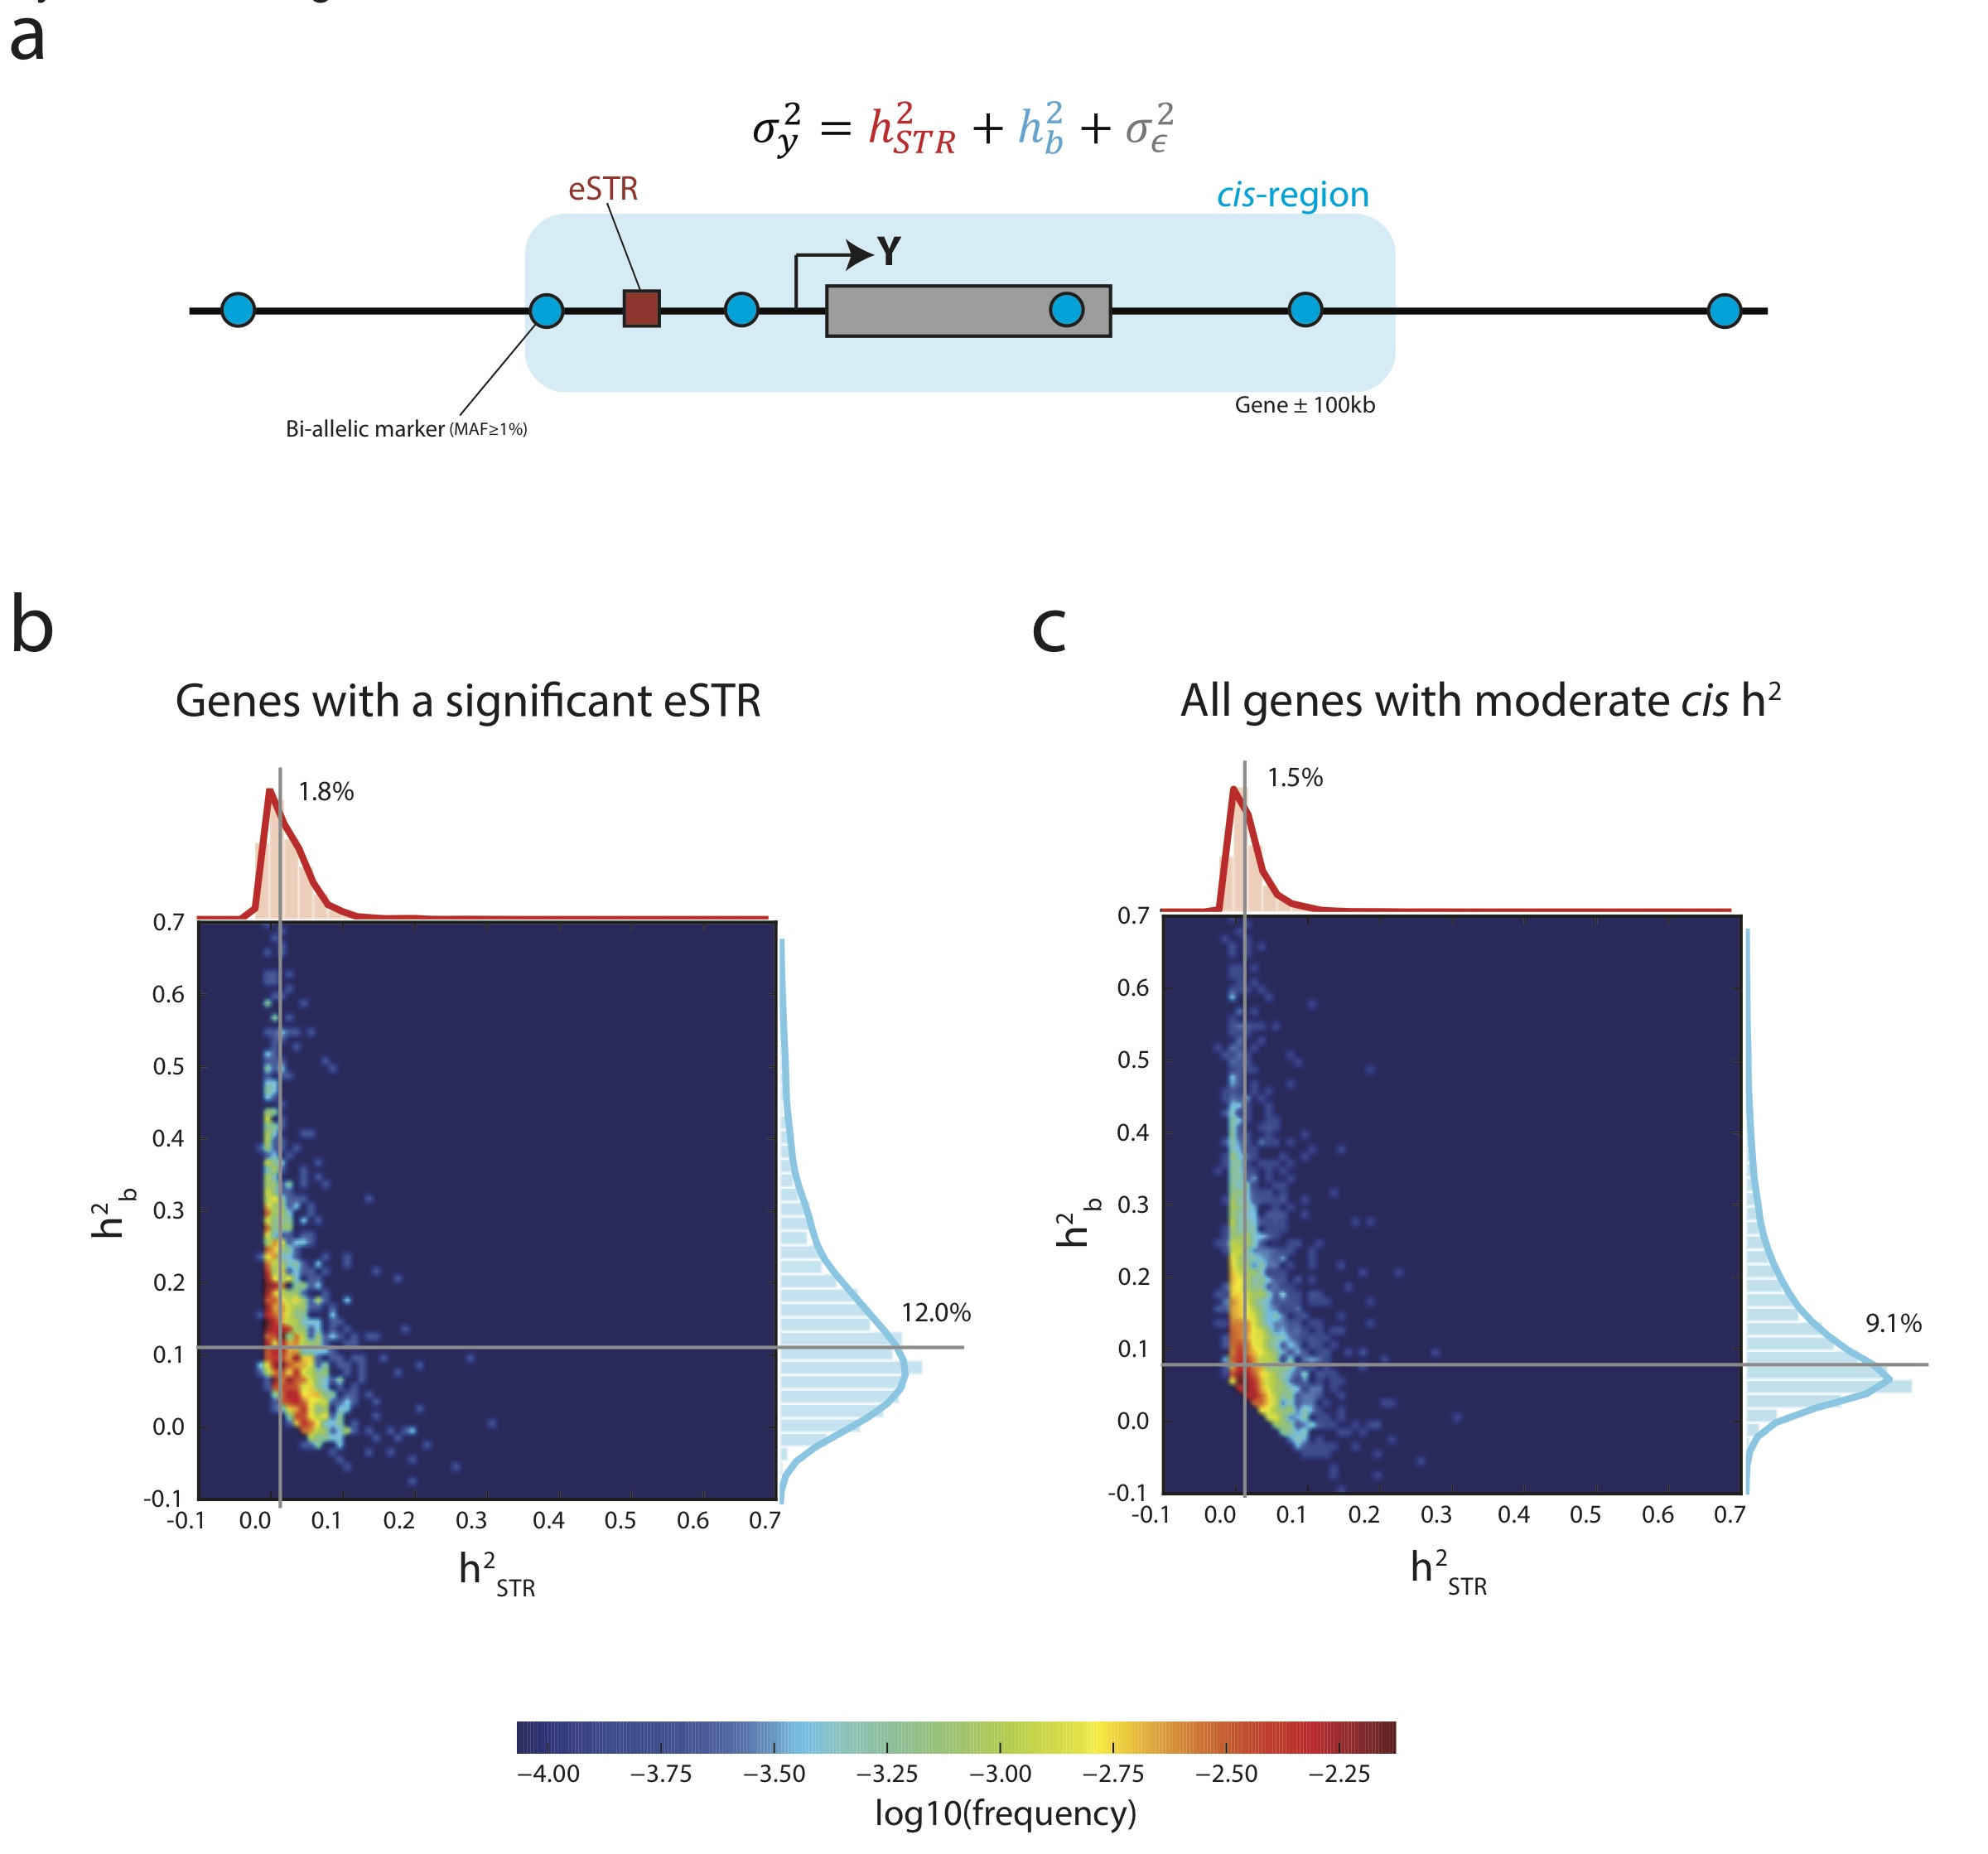
\includegraphics[width=0.7\textwidth]{Figures/Chapter4/Fig2}
\caption{\textbf{Variance partitioning using linear mixed models} \textbf{(a)} The normalized variance of the expression of gene Y was modeled as the contribution of the best eSTR and all common bi-allelic markers in the cis region (±100kb from the gene boundaries) \textbf{(b-c)} Heatmaps show the joint distributions of variance explained by eSTRs and by the cis region. Gray lines denote the median variance explained \textbf{(b)} Variance partitioning across genes with a significant eSTR in the discovery set and \textbf{(c)} Variance partitioning across genes with moderate cis heritability. }
\end{figure}

\subsection{The effect of eSTRs in the context of individual SNP eQTLs}
To further assess the contribution of eSTRs in the context of other variants, we also inspected the relationship between eSTRs and individual cis-SNP eQTLs (eSNPs). We performed a traditional eQTL analysis using the whole genome sequencing data for 311 individuals that were part of the discovery set to identify common eSNPs [minor allele frequency (MAF) $\geq$5\%] within 100kb of each gene. This process identified 4,290 genes with an eSNP (gene-level FDR$\leq$5\%). We then re-analyzed the eSTR association signals while conditioning on the genotype of the most significant eSNP (\textbf{Fig. \ref{fig:estrfig3}a}). For each eSTR, we ascertained the subset of individuals that were homozygous for the major allele of the lead eSNP in the region. If the eSTR simply tags this eSNP, its conditioned effect should be randomly distributed compared to the unconditioned effect. Alternatively, if the eSTR is causal, the direction of the conditioned effect should match that of the original effect. We conducted this analysis for eSTR loci with at least 25 individuals homozygous for the lead eSNP and for which these individuals had at least two unique STR genotypes (1,856 loci). After conditioning on the lead eSNP, the direction of effect for 1,395 loci (75\%) was identical to that in the original analysis (sign test $p<4.2 \times 10^{-109}$) and the effect sizes were significantly correlated ($R=0.52$; $p=3.2\times10^{-130}$) (\textbf{Fig. \ref{fig:estrfig3}b}). This further supports the additional role of eSTRs beyond traditional cis-eQTLs. 

\begin{figure}[h!]
\centering
\label{fig:estrfig3}
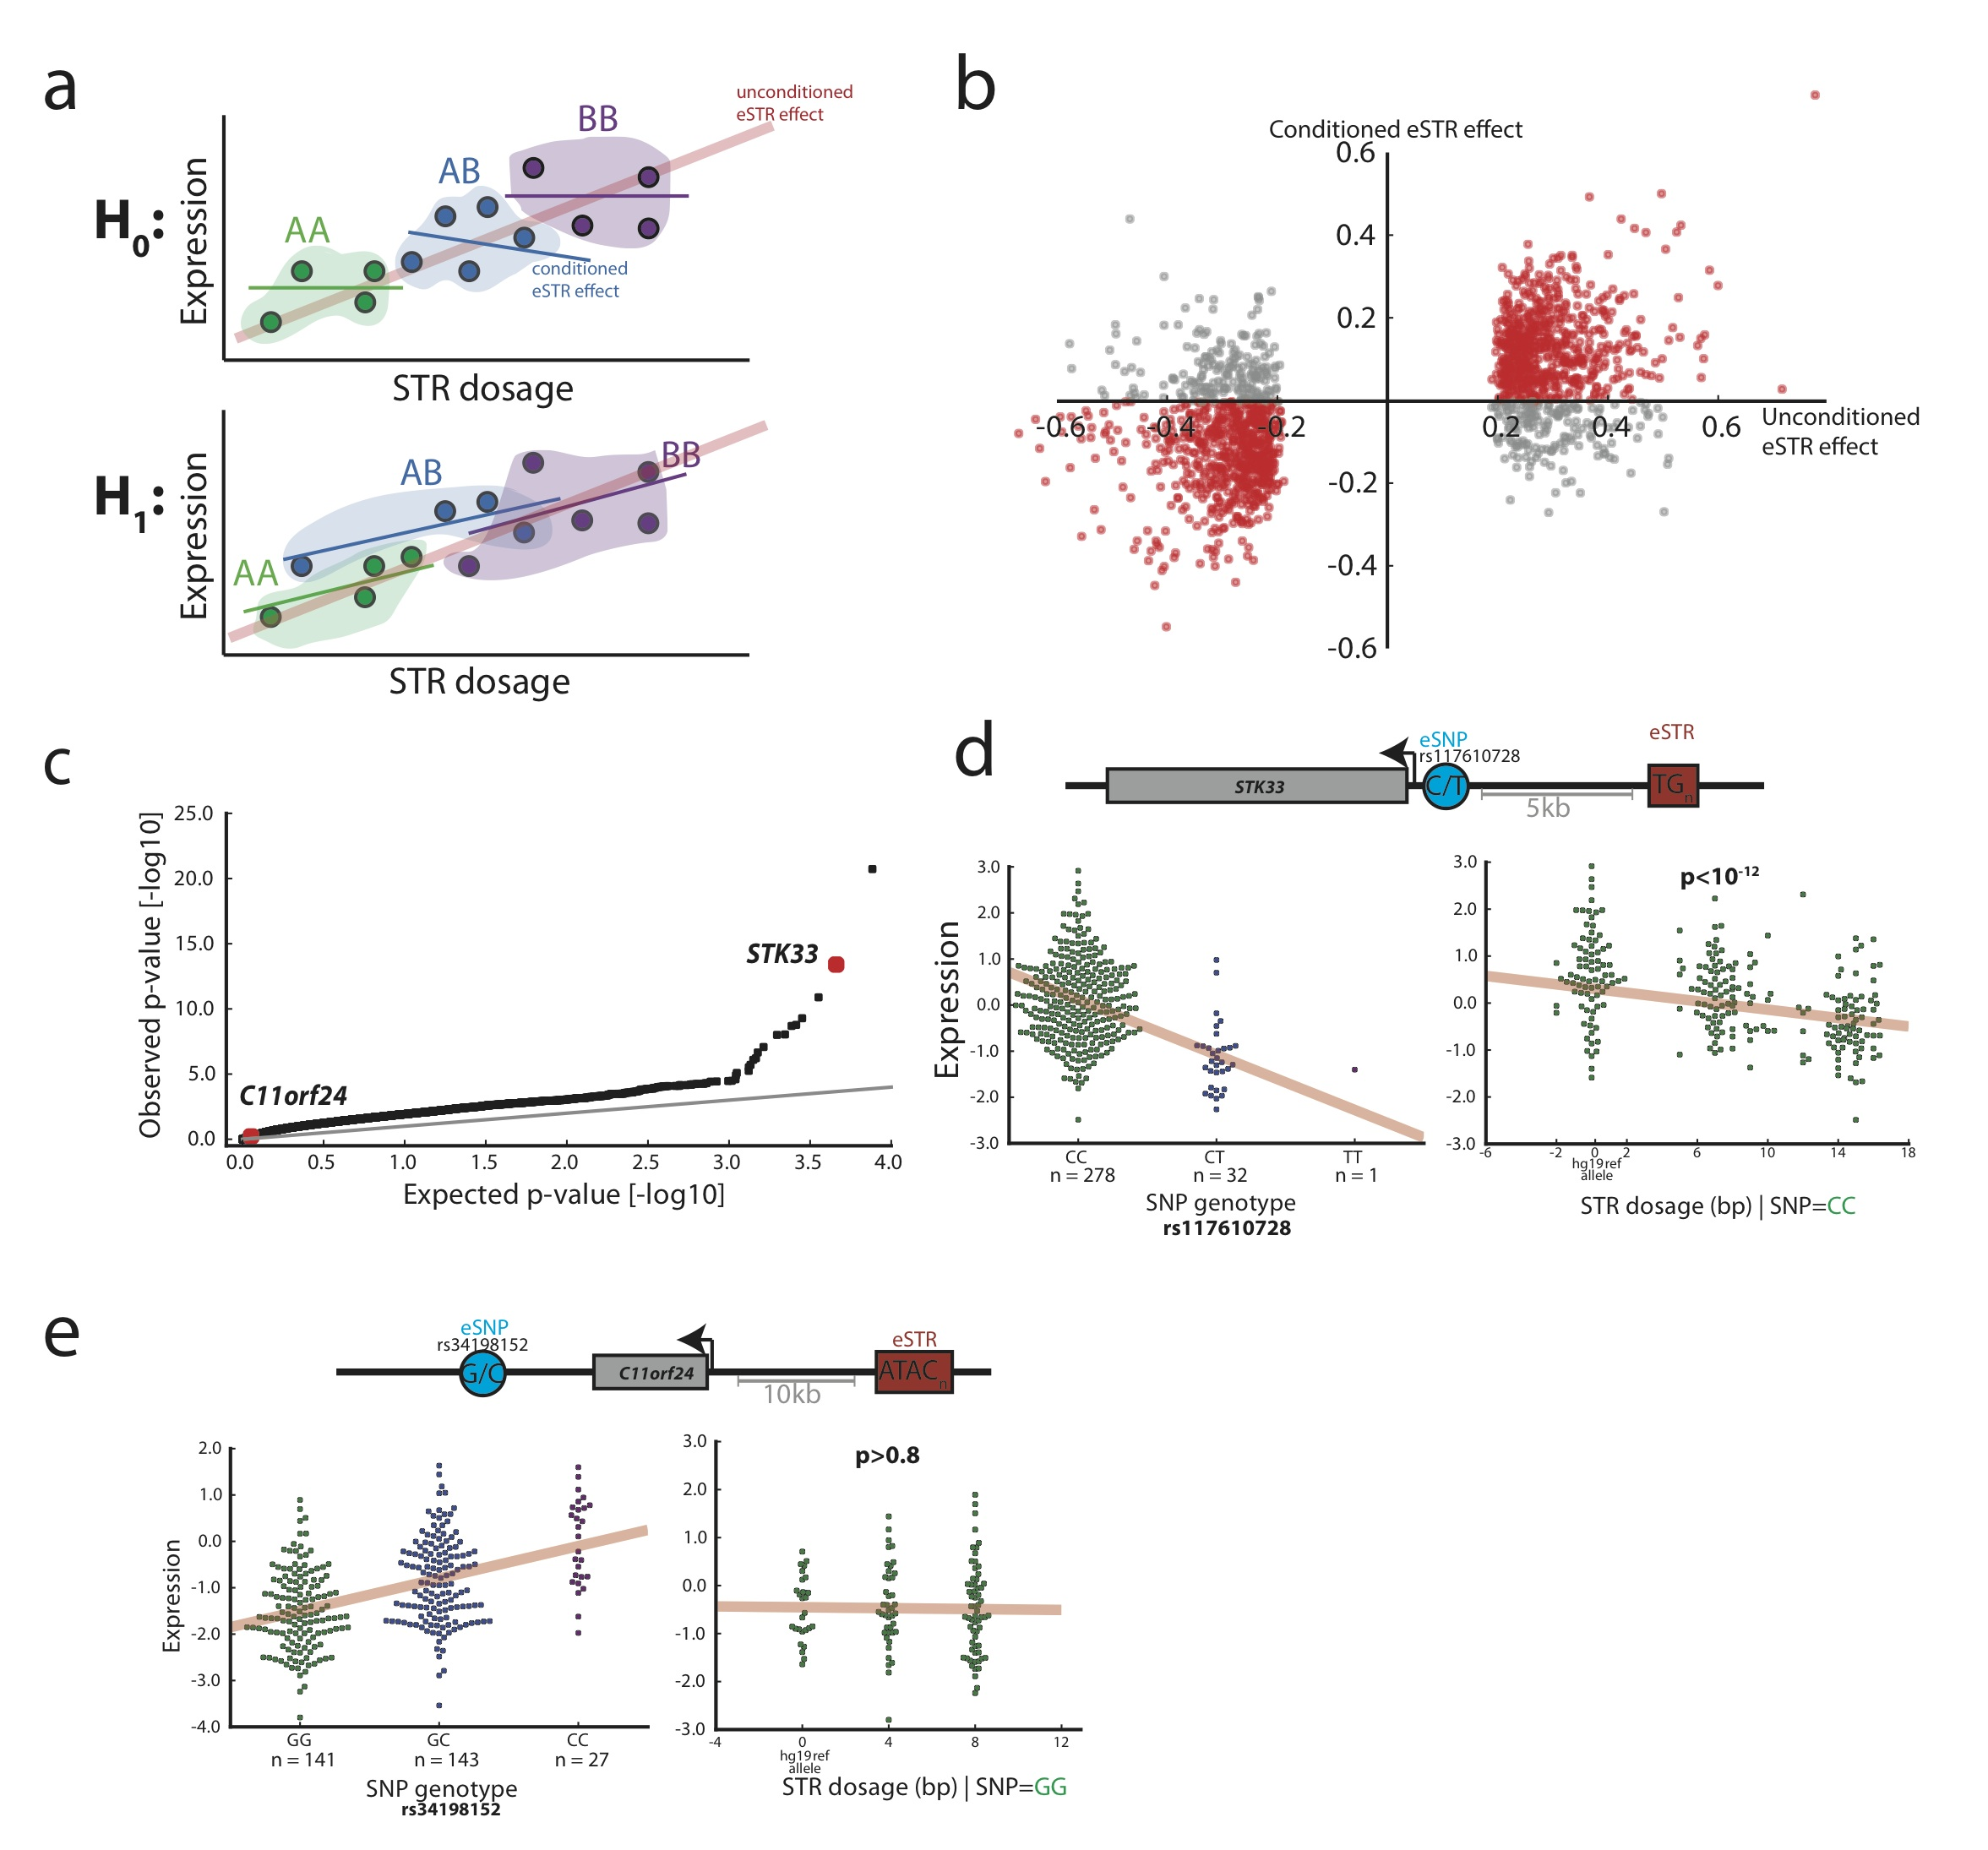
\includegraphics[width=0.7\textwidth]{Figures/Chapter4/Fig3}
\caption{\textbf{eSTR associations in the context of eSNPs} \textbf{(a)} Schematic of the eSTR effect versus the effect conditioned on the lead eSNP genotype. Under the null expectation, the original association (red line) comes from mere tagging of eSNPs. Thus, the eSTR effect disappears when restricting to a group of individuals (dots) with the same eSNP genotype (colored patches). Under the alternative hypothesis, the effect is concordant between the original and conditioned associations \textbf{(b)} The original eSTR effect versus the conditioned eSTR effect. Red points denote eSTRs whose direction of effect was concordant in both datasets and gray points denote eSTRs with discordant directions \textbf{(c)} Quantile-quantile plot of p-values from ANOVA testing of the explanatory value of eSTRs beyond that of eSNPs \textbf{(d)} \emph{STK33} is an example of a gene for which the eSTR (red rectangle) has a strong explanatory value beyond the lead eSNP (blue circle) based on ANOVA. When conditioning on individuals that are homozygous for the ``C'' eSNP allele (bottom left, green dots), the STR dosage still shows a significant effect (bottom right) \textbf{(e)} \emph{C11orf24} is an example of a gene for which the eSTR was part of the discovery set but did not pass the ANOVA threshold. After conditioning on individuals that are homozygous for the ``G'' eSNP allele (bottom left, green dots), the STR effect is lost (bottom right).}
\end{figure}

We also found that hundreds of eSTRs in the discovery set provide additional explanatory value for gene expression beyond the lead eSNP. ANOVA model comparison showed that for 23\% of the cases, a model with an eSTR significantly improved the explained variance of gene expression over considering only the lead eSNP (FDR$<$5\%) (\textbf{Fig. \ref{fig:estrfig3}c-e} and \textbf{Online Methods \ref{sec:estrolm}}). Combined with the 183 genes with an eSTR but no significant eSNP, these results show that at least 30\% of the eSTRs identified by our initial scan cannot be fully attributed to tagging of the lead eSNP. Given the reduced quality of STR compared to SNP genotypes, this analysis is likely to underestimate the true contribution of STRs. Nonetheless, our results show concrete examples for hundreds of associations in which the eSTR increases the variance explained by the lead eSNP.

\subsection{Integrative genomic evidence for a functional role of eSTRs}
To provide further evidence of their regulatory role, we analyzed eSTRs in the context of functional genomics data. First, we assessed the potential functionality of STR regions by measuring signatures of purifying selection, since previous studies reported that putatively causal eSNPs are slightly enriched in conserved regions \cite{GaffneyVeyrierasDegnerEtAl2012}.  We inspected the sequence conservation \cite{PollardHubiszRosenbloomEtAl2010} across 46 vertebrates in the sequence upstream and downstream of the eSTRs in our discovery dataset (\textbf{Fig. \ref{fig:estrfig4}a}). To tune the null expectation, we matched each tested eSTR to a random STR that did not reach significance in the association analysis but had a similar distance to the nearest transcription start site (TSS). The average conservation level of a $\pm$500bp window around eSTRs was slightly but significantly higher (p$<$0.03) compared to control STRs. Tightening the window size to shorter stretches of $\pm$50bp showed a more significant contrast in the conservation scores of the eSTRs versus the control STRs (p$<$0.01) (\textbf{Fig. \ref{fig:estrfig4}a} inset), indicating that the excess in conservation comes from the vicinity of the eSTR loci. Taken together, these results show that eSTRs discovered by our association pipeline reside in regions exposed to relatively higher purifying selection, further suggesting a functional role.

eSTRs substantially co-localize with functional elements. They show the strongest enrichment closest to transcription start sites (\textbf{Fig. \ref{fig:estrfig4}b}) and to a lesser extent in or near predicted enhancers (\textbf{Supplementary Fig. \ref{fig:estrsupfig10}}). We also inspected the co-localization of eSTRs with histone modifications as annotated by the Encode Consortium \cite{ConsortiumDunhamKundajeEtAl2012} in LCLs. eSTRs were strongly enriched in peaks of histone modifications associated with regulatory regions (H3K4me3, H3K27ac, H3K9ac) and transcribed regions (H3K36me3) and were depleted in repressed regions (H3K27me3) (\textbf{Fig. \ref{fig:estrfig4}b}). To test the significance of these signals, we constructed a null distribution for each histone modification by measuring the co-localization of eSTRs with randomly shifted histone peaks similar to the procedure used by Trynka et al \cite{TrynkaWestraSlowikowskiEtAl2014}. This null distribution controls for the co-occurrence of eSTRs and histone peaks due to their proximity to other causal variants. We found eSTR/histone co-localizations were significant (weakest p$<$0.01) after the peak shifting procedure, suggesting that these results stem from the eSTRs themselves (\textbf{Supplementary Table \ref{tab:estrsuptab8}}). We also performed a peak-shifting analysis using ChromHMM annotations \cite{ErnstKellis2012} (\textbf{Fig. \ref{fig:estrfig4}c}) which indicated that eSTRs are most strongly enriched in weak-promoters (p$<$0.002) and weak-enhancers (p$<$0.004). Again, this analysis shows overlap of eSTRs with elements that are predicted to regulate gene expression.  

We also found that eSTR length variations are more likely to modulate the presence of certain histone marks (\textbf{Online Methods \ref{sec:estrolm}} and \textbf{Supplementary Fig. \ref{fig:estrsupfig11}}). We introduced different eSTR alleles to GERV \cite{ZengHashimotoKangEtAl2015a}, a machine learning approach that examines the effect of DNA sequence on histone marks. This process found that eSTRs have significantly greater effects than control STRs on predicted regulatory regions (H3K4me3 p=0.00109, DNAseI hypersensitivity p=0.00045, H3K9ac p=0.00462) and transcribed regions (H3K36me3 p=0.01336). These results are consistent with the analysis of chromatin modifications above. Importantly, since the input material for this analysis is solely STR variations that are independent of any linked variants, these results provide an orthogonal piece of evidence for the functionality of eSTRs and suggest histone mark modulation as a potential mechanism. 

\begin{figure}[h!]
\centering
\label{fig:estrfig4}
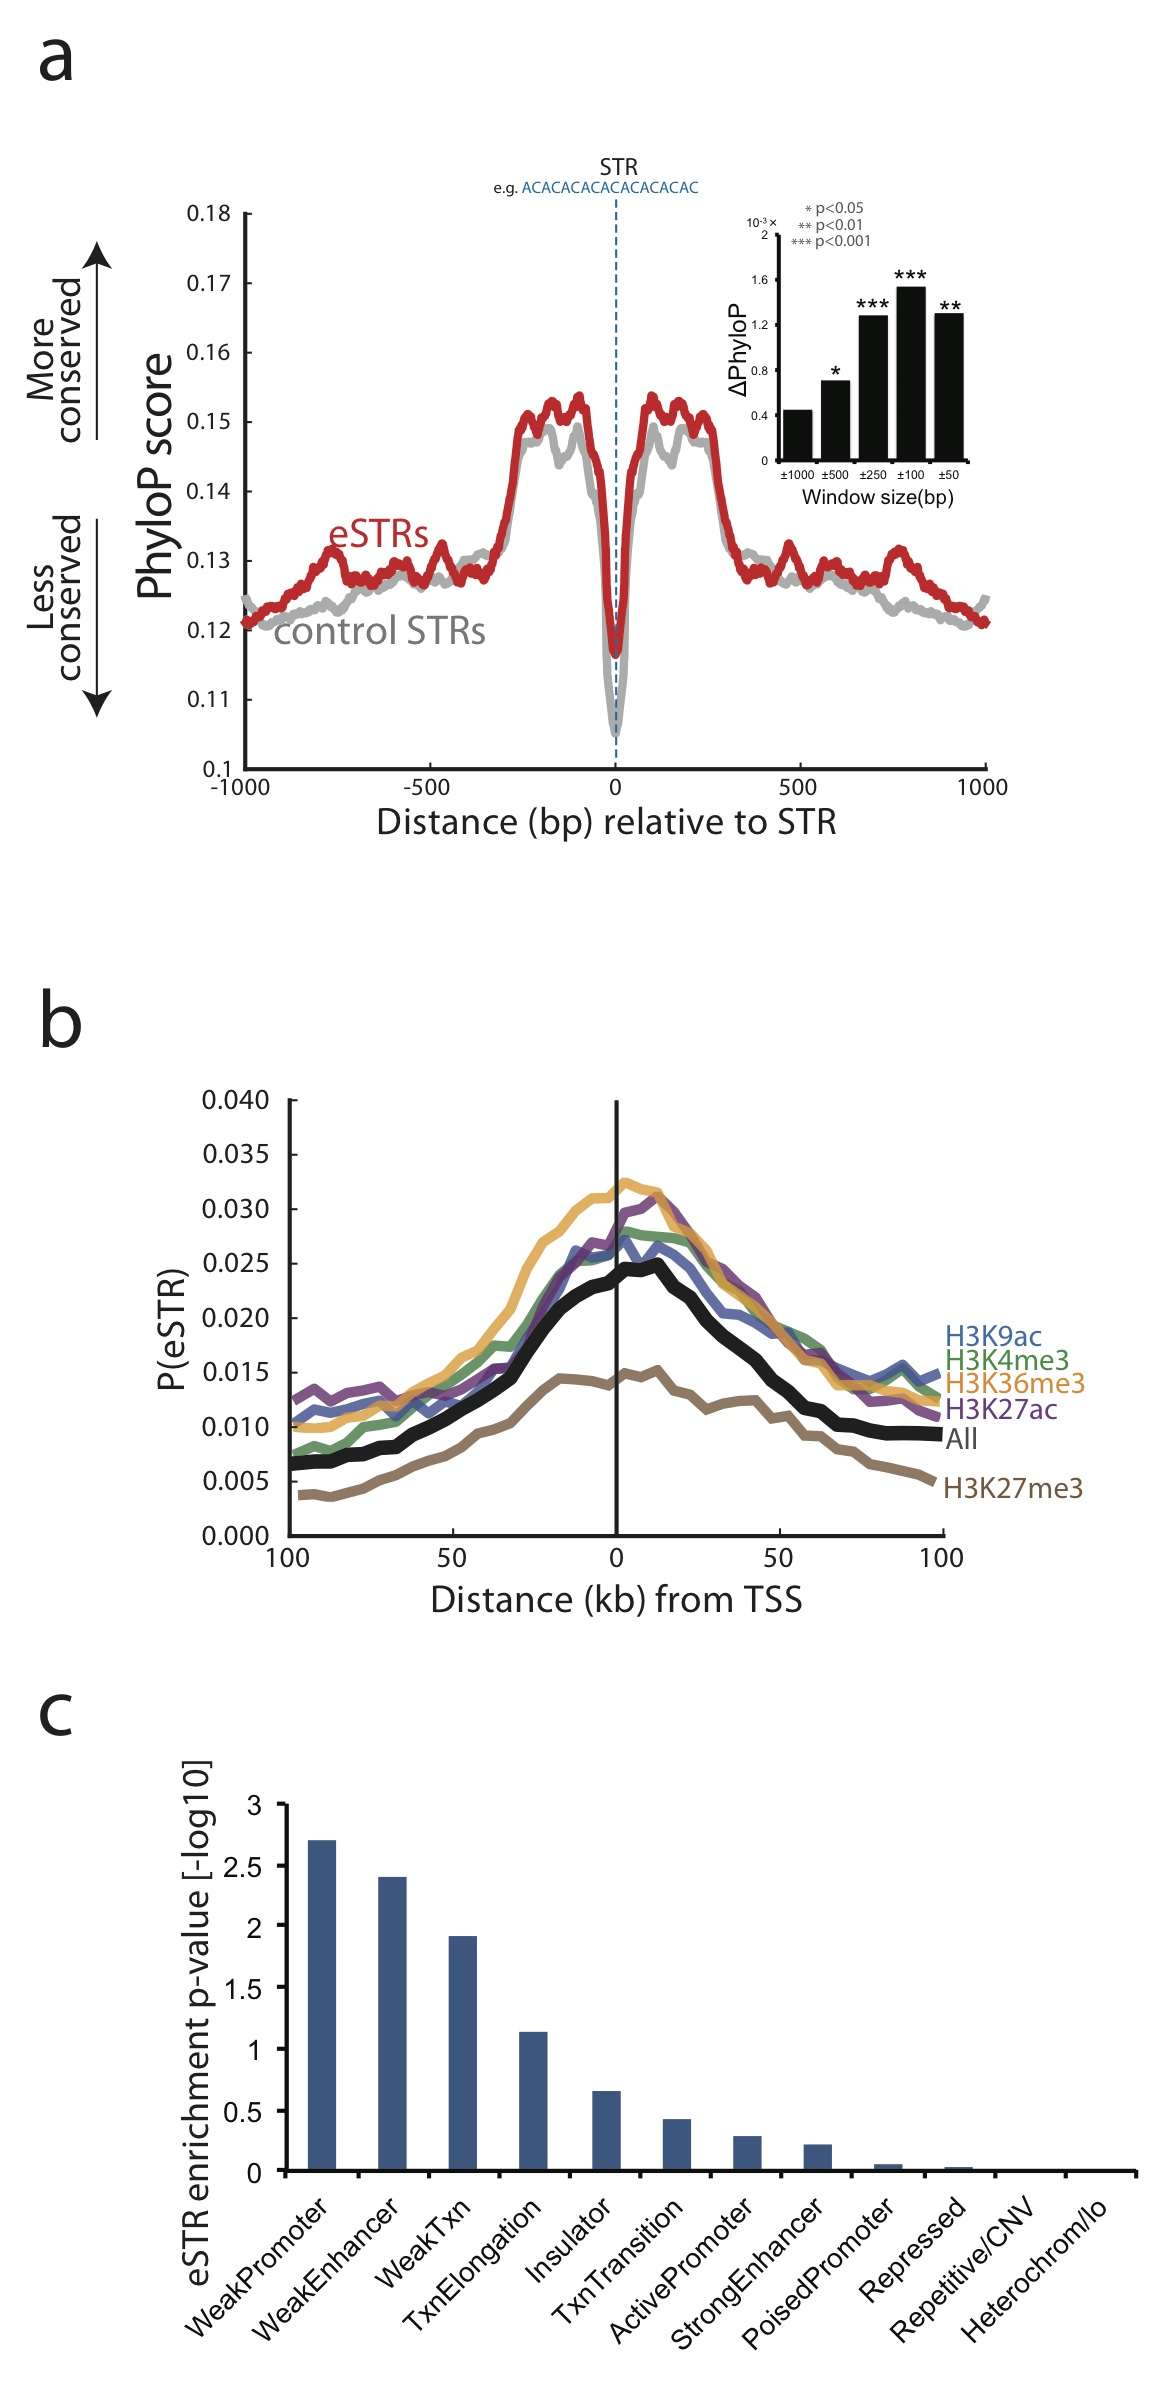
\includegraphics[width=0.4\textwidth]{Figures/Chapter4/Fig4}
\caption{\textbf{Conservation and epigenetic analysis of eSTR loci} \textbf{(a)} Median PhyloP conservation score as a function of distance from the STR. Red: eSTR loci, gray: matched control STRs. Inset: the difference in the PhyloP conservation score between eSTRs and matched control STRs as a function of window size around the STR. \textbf{(b)} The probability that an STR scores as an eSTR in the discovery set as a function of distance from the transcription start site (TSS). eSTRs show clustering around the TSS (black line). Conditioning on the presence of a histone mark (colored lines) significantly modulated the probability that an STR is an eSTR \textbf{(c)} The enrichment of eSTRs in different chromatin states.}
\end{figure}

\subsection{The potential role of eSTRs in human conditions}
Encouraged by the evidence for the regulatory role of eSTRs, we wondered about their potential involvement in clinically-relevant conditions. First, we tested whether genes implicated by previous GWAS scans listed in the NHGRI GWAS catalog \cite{WelterMacArthurMoralesEtAl2014} are enriched for eSTR genes. We focused on seven complex disorders: rheumatoid arthritis, Crohn's disease, type 1 diabetes, type 2 diabetes, blood pressure, bi-polar disorder, and coronary artery disease. The first three conditions have a strong autoimmune component, rendering them more relevant to the LCL data used for eSTR discovery. To create a proper null, we compared the overlap of eSTR genes to randomly chosen sets of genes matched to the tested GWAS genes on both gene expression level in LCLs and on cis heritability.

We found that GWAS genes for Crohn's disease are significantly (p$<$0.001) enriched for eSTR hits (\textbf{Figure \ref{fig:estrfig5}a} and \textbf{Supplementary Fig. \ref{fig:estrsupfig12}}). Moderate enrichment for eSTRs (p=0.074) was found in GWAS genes for rheumatoid arthritis, consistent with the known role of immune function in these traits. Enrichments were 2-3 times higher for autoimmune diseases than for the other conditions (average overlap: 6\%). Interestingly, for seven overlapping genes, the eSTRs explained more variance in gene expression than the lead eSNP of the gene. Furthermore, for close to thirty genes, a joint model of the lead eSTR and eSNP explained significantly more variance in gene expression than the eSNP alone, raising the possibility of an etiological role. 

Next, we performed an association study using eSTRs to further test the hypothesis that eSTRs underlie clinically relevant phenotypes. For this, we turned to $\sim$1,700 unrelated individuals that were sequenced to medium coverage (6x) with 100bp paired-end reads using Illumina as part of the TwinsUK cohort of the UK10K project \cite{ConsortiumWalterMinEtAl2015} and were phenotyped for a wide array of quantitative traits, primarily blood metabolites and anthropometric traits. While most of these conditions are not directly related to the immune system, we hypothesized that similar to other eQTLs \cite{ArdlieDelucaSegreEtAl2015}, some of the discovered eSTRs are shared across tissues and could play a role in additional tissues. After genotyping STRs with lobSTR, we tested for association between eSTRs and each of the 38 reported phenotypes, while controlling for sex, age, and population structure. To enrich for STR loci that are likely to be causal for gene expression variation, we restricted analysis to eSTRs that significantly improved the explained variance of gene expression over a model with the lead eSNP alone. In total, we obtained 499 eSTRs after applying this condition and excluding eSTRs that were genotyped in $<$1000 individuals. 

We identified 12 significant associations (FDR per phenotype$<$10\%) between eSTRs and the clinical phenotypes in the TwinsUK data (\textbf{Figure \ref{fig:estrfig5}b} and \textbf{Supplementary Table \ref{tab:estrsuptab9}}). Only one association overlapped a known GWAS hit: an AAAC repeat on 4p16 was associated with decreased expression of \emph{SLC2A9} and increased uric acid in serum samples of the TwinsUK, which matches previous studies with SNPs \cite{DoringGiegerMehtaEtAl2008,VitartRudanHaywardEtAl2008,WallaceNewhouseBraundEtAl2008,ShinFaumanPetersenEtAl2014}. The other 11 associations involved changes in blood metabolites such as albumin and C-reactive protein and physical traits such as diastolic blood pressure and FEV1 lung function and have yet to be described before in GWAS catalogs, suggesting novel loci. We caution that full validation of each of these associations will require replication in additional cohorts. Nonetheless, as we were mainly interested in the overall trend for eSTRs, we repeated the association of the 38 phenotypes in the TwinsUK cohort with a similar number of random STR loci matched on distance to transcription start sites, repeat motif, and number of genotyped samples. One hundred rounds of bootstrapping showed that eSTRs produced significantly more associations than the matched STR controls (mean for controls: 6.8 associations at FDR$<$10\%, z-test, $p<1.8\times 10^{-16}$). Repeating this test with a more stringent FDR of 5\% revealed a similar picture: the eSTRs produced 6 associations passing this threshold (Supplementary Table 9), significantly more that the matched STR controls (mean for controls: 3.2 associations at FDR$<$5\%, $p<1.1\times10^{-5}$). Taken together, our results show that eSTR signals are enriched in clinical phenotypes both in known and potentially novel GWAS hits. These results could inform future efforts for disease mapping studies.

\begin{figure}[h!]
\centering
\label{fig:estrfig5}
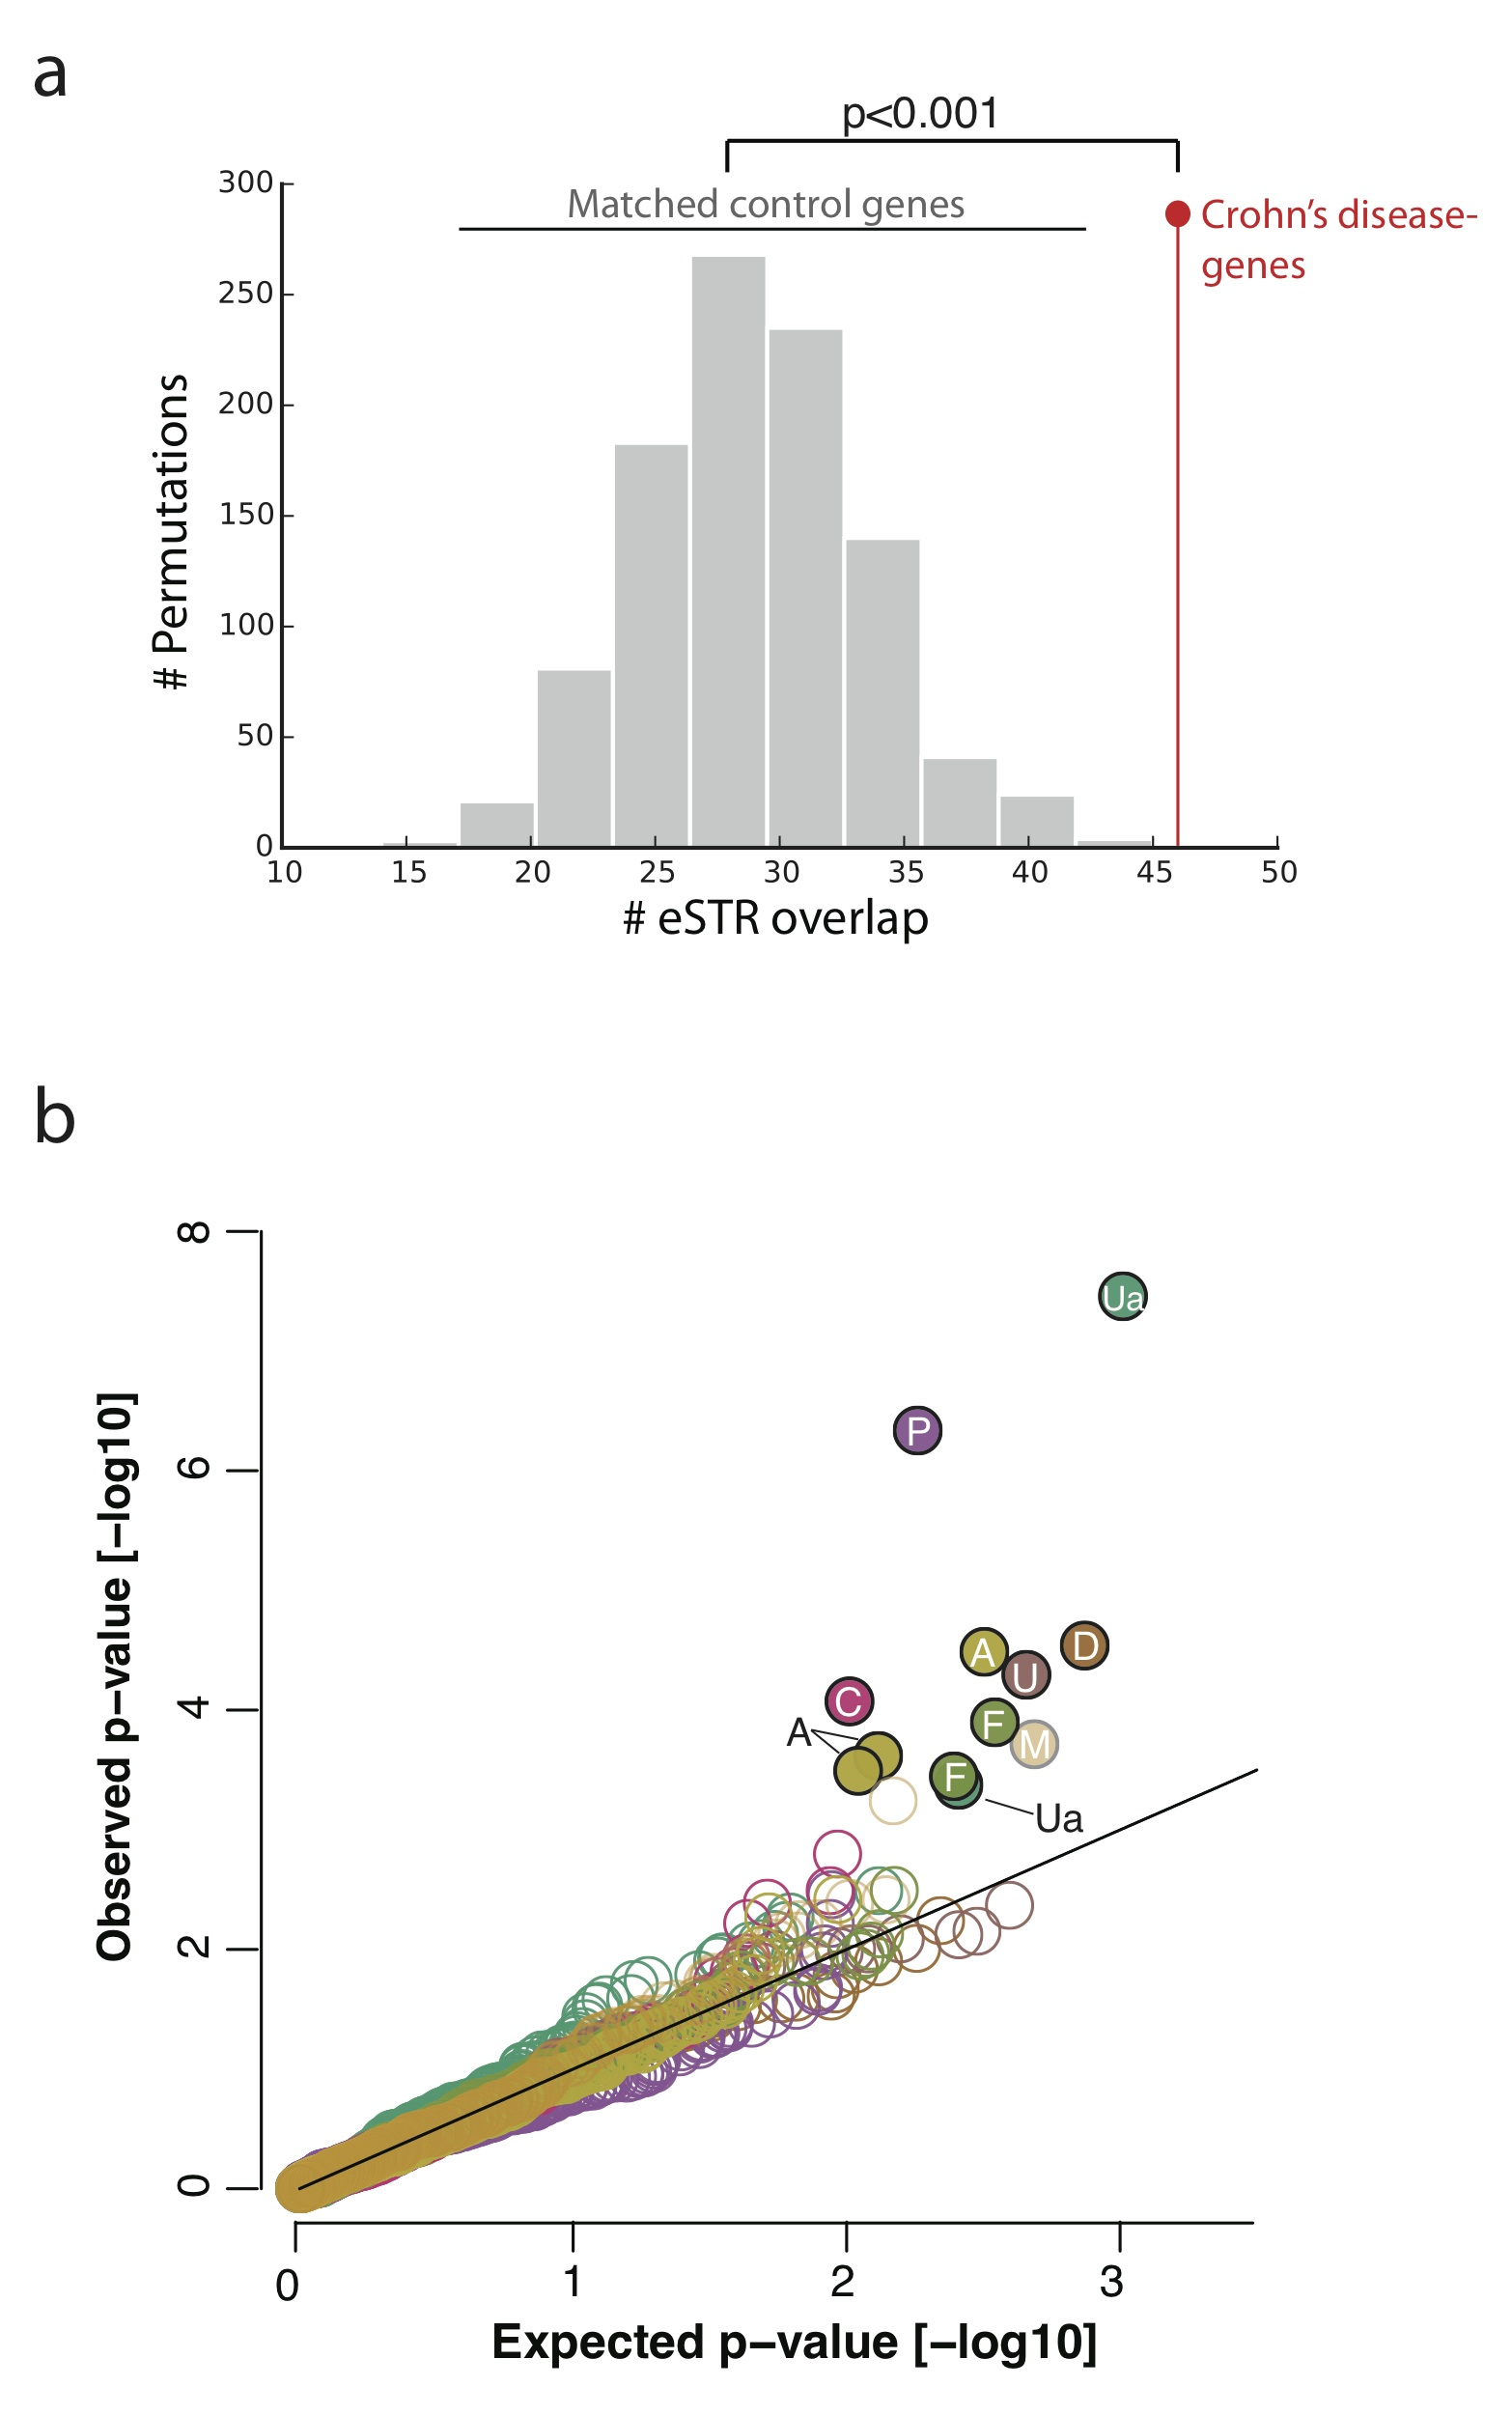
\includegraphics[width=0.5\textwidth]{Figures/Chapter4/Fig5}
\caption{\textbf{Association of eSTRs with clinical phenotypes} \textbf{(a)} The overlap between eSTRs and Crohn's disease GWAS genes (red) versus random subsets of genes (gray) matched on expression and heritability profiles in LCLs \textbf{(b)} quantile-quantile plots of eSTR associations in the TwinsUK data. Only traits with significant (FDR<0.1) associations are plotted. Closed circles: significant, open circles: non-significant. A: albumin; C: C-reactive protein; D: diastolic blood pressure, F: FVC, M: mean corpuscular volume, P: phosphate, U: Urea, Ua: Uric acid.}
\end{figure}

\section{Discussion}
Repetitive elements have often been considered as neutral with no phenotypic consequences \cite{GemayelChoBoeynaemsEtAl2012}. This coupled with the technical difficulties in analyzing these regions has led large-scale genetic studies to largely overlook the putative contribution of repeats to human phenotypes. Our study focused on short tandem repeats, one of the most polymorphic classes of loci that comprise 1\% of the human genome. Despite being less abundant than SNPs, previous studies have shown that STRs are enriched in promoters and enhancers, where they frequently induce multiple base-pair variations, increasing the prior expectation of their ability to explain gene expression variation. Following these observations, we conducted a genome-wide scan for the contribution of STRs to gene expression. Our scan identified over 2,000 potential eSTRs and found that eSTRs contribute on average about 10-15\% of the cis-heritability of gene expression attributed to common (MAF$\geq$1\%) polymorphisms. Functional genomics analyses provided further support for the predicted causal role of eSTRs. Finally, we found that eSTRs are enriched in clinically relevant phenotypes. 

We hypothesize that there are more eSTRs to find in the genome as our analysis had several technical limitations. First, the higher genotyping error rates for STRs compared to SNPs limited our power to detect eSTRs and likely downwardly biased their estimated contribution in the LMM and ANOVA analyses. In addition, about 10\% of STR loci in the genome could not be analyzed because they are too long to be spanned by current sequencing read lengths(Willems et al. 2014). Second, based on previous findings in humans \cite{GebhardtZankerBrandt1999,ShimajiriArimaTanimotoEtAl1999,ContenteDittmerKochEtAl2002}, our association tests focused on a linear relationship between STR length and gene expression. However, experimental work in yeast reported that certain loci exhibit non-linear relationships between STR length and expression \cite{VincesLegendreCaldaraEtAl2009}, which are unlikely to be captured in our current analysis. Finally, our association pipeline takes into account only the length polymorphisms of STRs and cannot distinguish the effect of sequence variations inside STR alleles with identical lengths (dubbed homoplastic alleles \cite{WeberBroman2001}). Addressing these technical complexities would likely require phased STR haplotypes and longer sequence reads that are currently unavailable for large sample sizes. We envision that recent advancements in sequencing technologies \cite{ChaissonHuddlestonDennisEtAl2015} will further expand the catalog of eSTRs.  

Despite these technical limitations, our findings show that repetitive elements in the human genome extensively contribute to expression variation and are enriched in clinically relevant phenotypes. Our results are consistent with a recent study that reported that haplotypes of common SNPs, which capture genetic variants poorly tagged by current genotype panels, can explain substantially more heritability than common SNPs alone \cite{BhatiaGusevLohEtAl2015}. We anticipate that integrating the analysis of repetitive elements, specifically STR variations, will explain additional heritability and will lead to the discovery of new genetic variants relevant to human conditions.

\section{Acknowledgements}
M.G. was supported by the National Defense Science and Engineering Graduate Fellowship. Y.E. holds a Career Award at the Scientific Interface from the Burroughs Wellcome Fund. This study was supported by a gift from Andria and Paul Heafy (Y.E), NIJ grant 2014-DN-BX-K089 (Y.E, T.W), and NIH grants 1U01HG007037 (H.Z), R01MH084703(J.P), R01HG006399 (A.L.P), HG006696 (A.J.S), DA033660 (A.J.S), and MH097018 (A.J.S), and a research grant 6-FY13-92 from the March of Dimes Foundation (A.J.S). We thank Tuuli Lappalainen, Alon Goren, Tatsu Hashimoto, and Dina Zielinksi for useful comments and discussions.

\section{Author Contributions}
M.G. and Y.E. conceived the study. M.G., T.W., H.Z., B.M., and Y.E. performed analyses. A.G. performed experimental work to generate high coverage sequencing data for promoter STRs. S.G., M.J.D., A.L.P., and J.K.P. provided statistical input. A.J.S. contributed data and analyses. M.G., T.W., and Y.E. authored the manuscript.

\section{Online Methods}
\label{sec:estrolm}

\subsection{Genotype datasets}
lobSTR genotypes were generated for the phase 1 individuals from the 1000 Genomes Project as described in \cite{WillemsGymrekHighnamEtAl2014}. Variants from the 1000 Genomes Project phase 1 release were downloaded in VCF format from the project website. HapMap genotypes were used to correct association tests for population structure. Genotypes for 1.3 million SNPs were downloaded for draft release 3 from the HapMap Consortium. SNPs were converted to hg19 coordinates using the liftOver tool and filtered using Plink \cite{PurcellNealeTodd-BrownEtAl2007} to contain only the individuals for which both expression array data and STR calls were available. Throughout this manuscript, all coordinates and genomic data are referenced according to hg19.

\subsection{Targeted sequencing of promoter region STRs}
We used a previously published method using capture and high-throughput sequencing \cite{GuilmatreHighnamBorelEtAl2013} to sequence 2,472 STRs located in gene promoters (TSS $\pm$ 1kb) in 120 HapMap individuals of European (58 CEU individuals) and African (62 YRI individuals) ancestry. Briefly, the method uses a custom Nimblegen EZ Capture system to enrich the genomic sequence flanking, and sometimes including, the target STRs to be genotyped prior to sequencing using an Illumina Hiseq2000 instrument. We multiplexed 24 individuals per sequencing lane and utilized 100bp single-end reads. We used lobSTR version 3.0.3 to genotype STRs in these samples.

\subsection{Expression datasets}
RNA-sequencing datasets from 311 HapMap lymphoblastoid cell lines for which STR and SNP genotypes were also available were obtained from the gEUVADIS Consortium. Raw FASTQ files containing paired end 100bp Illumina reads were downloaded from EBI. The hg19 Ensembl transcriptome annotation was downloaded as a GTF file from the UCSC Genome Browser \cite{KentSugnetFureyEtAl2002,KarolchikBarberCasperEtAl2014} ensGene table. The RNA-sequencing reads were mapped to the Ensembl transcriptome using Tophat v2.0.7 \cite{TrapnellPachterSalzberg2009} with default parameters. Gene expression levels were quantified using Cufflinks v2.0.2 \cite{TrapnellRobertsGoffEtAl2012} with default parameters and supplied with the GTF file for the Ensembl reference version 71. Genes with median FPKM of 0 were removed, leaving 23,803 genes. We restricted analysis to protein coding genes, giving 15,304 unique Ensembl genes. Expression values were quantile-normalized to a standard normal distribution for each gene.

The replication set consisted of Illumina Human-6 v2 Expression BeadChip data from 730 HapMap lymphoblastoid cell lines from the EBI website. These datasets contain two replicates each for 730 unrelated individuals from 8 HapMap populations (YRI, CEU, CHB, JPT, GIH, MEX, MKK, LWK) and were generated as described by Stranger et al. \cite{StrangerNicaForrestEtAl2007}. Background corrected and summarized probeset intensities (by Illumina software) contained values for 7,655 probes. Additionally, probes containing common SNPs were removed \cite{Barbosa-MoraisDunningSamarajiwaEtAl2010}. Only probes with a one-to-one correspondence with Ensembl gene identifiers were retained. We removed probes with low concordance across replicates (Spearman correlation $\leq$ 0.5). In total we obtained 5,388 probes for downstream analysis.

Each probe was quantile-normalized to a standard normal distribution across all individuals separately for each replicate and then averaged across replicates. These values were quantile-normalized to a standard normal distribution for each probe.

\subsection{eQTL association testing}
Expression values were adjusted for individual sex, individual population membership, gene expression heterogeneity, and population structure (\textbf{Supplementary Note \ref{sec:estrsupnote}}). Adjusted expression values were used as input to the eSTR analysis. To restrict to STR loci with high quality calls, we filtered the call set to contain only loci where at least 50 of the 311 samples had a genotype call. To avoid outlier genotypes that could skew the association analysis, we removed any genotypes seen less than three times. If only a single genotype was seen more than three times, the locus was discarded. To increase our power, we further restricted analysis to the most polymorphic loci with heterozygosity of at least 0.3. This left 80,980 STRs within 100kb of a gene expressed in our LCL dataset.

A linear model was used to test for association between normalized STR dosage and expression for each STR within 100kb of a gene. Dosage was defined as the sum of the deviations of the STR allele lengths from the hg19 reference. For example, if the hg19 reference for an STR is 20bp and the two alleles called are 22bp and 16bp, the dosage is equal to (22-20)+(16-20) = -2bp. STR genotypes were zscore-normalized to have mean 0 and variance 1. For genes with multiple transcripts, we defined the transcribed region as the maximal region spanned by the union of all transcripts. The linear model for each gene is given by:

\begin{equation}
\vec{y}_g = \alpha_g + \beta_{j,g}\vec{x}_j + \vec{\epsilon}_{j,g}
\end{equation}

where $\vec{y_g} = (y_{g,1},\hdots, y_{g,n})^T$  with $y_{g,i}$ the normalized covariate-corrected expression of gene $g$ in individual $i$, $n$ is the number of individuals, $\alpha_g$ is the mean expression level of homozygous reference individuals, $\beta_{j,g}$ is the effect of the allelic dosage of STR locus $j$ on gene $g$, $\vec{x_j} = (x_{j,1}, \hdots, x_{j,n})^T$ with $x_{j,i}$ the normalized allelic dosage of STR locus $j$ in the $i$th individual, and $\vec{\epsilon}_{j,g}$ is a random vector of length $n$ whose entries are drawn from $N(0, \sigma_{\epsilon, j, g}^2)$ where $\sigma_{\epsilon, j, g}^2$ is the unexplained variance after regressing locus $j$ on gene $g$. The association was performed using the OLS function from the Python statsmodels package. For each comparison, we tested $H_0: \beta_{j,g} = 0$ vs. $H_1: \beta_{j,g} \neq 0$ using a standard $t$-test. We controlled for a gene-level false discovery rate (FDR) of 5\% (see below).

\subsection{Controlling for gene-level false discovery rate}
We controlled for a gene-level FDR of 5\%, assuming that most genes have at most a single causal eSTR. For each gene, we determined the STR association with the best p-value. This p-value was adjusted using a Bonferroni correction for the number of STRs tested per gene to give a p-value for observing a single eSTR association for each gene. Performing separate permutations for each gene was computationally infeasible, and was found to give similar results to a simple Bonferroni correction on a subset of genes. We then used this list of adjusted p-values as input to the qvalue R package to determine all genes with FDR at most 5\%.

\subsection{Partitioning heritability using linear mixed models}
For each gene, we used a linear mixed model to partition heritability between the lead explanatory STR and other cis variants. We used a model of the form:

\begin{equation}
\vec{y}_g = \alpha_g + \beta_{j,g}\vec{x}_j + \vec{u}_g + \vec{\epsilon}_{j,g}
\end{equation}

where $\vec{y}_g$, $\alpha_g$, $\beta_{j,g}$, $\vec{x}_j$, and $\epsilon_{j,g}$ are as described above, $\vec{u}_g$ is a length $n$ vector of random effects and $\vec{u}_g \sim MVN(0, \sigma_{u_g}^2 K_g)$ with $\sigma_{u_g}^2$ the percent of phenotypic variance explained by cis bi-allelic variants for gene $g$, and $K_g$ is a standardized $n\times n $identity by state (IBS) relatedness matrix constructed using all common bi-allelic variants (MAF$\geq$ 1\%) reported by phase 1 of the 1000 Genomes Project within 100kb of gene g. This includes SNPs, indels, and several bi-allelic structural variants and is constructed as $K_g = \frac{1}{p} \sum_{i=0}^p \frac{1}{var(\vec{x}_i)}(\vec{x}_i - 1_nmean(\vec{x}_i))(\vec{x}_i-1_nmean(\vec{x}_i))^T$ where $p$ is the total number of variants considered, $\vec{x}_i$ is a length n vector of genotypes for variant $i$, and $1_n$ is a length $n$ vector of ones. Note the mean diagonal element of $K_g$ is equal to 1.

We used the GCTA program(Yang et al. 2011) to determine the restricted maximum likelihood estimates (REML) of $\beta_{j,g}$ and $\sigma_{u_g}^2$. To get unbiased values of $\sigma_{u_g}^2$, the -{}-reml-no-constrain option was used.

We used the resulting estimates to determine the variance explained by the STR and the cis region. We can write the overall phenotypic variance-covariance matrix as:

\begin{equation}
var(\vec{y}_g) = \beta_{j,g}^2var(\vec{x}_j) + \sigma_{u_g}^2K_g + \sigma_{\epsilon_{j,g}}^2I_n
\end{equation}

where $var(\vec{y}_g)$ is an $n \times n$ expression variance-covariance matrix with diagonal elements equal to 1, since expression values for each gene were normalized to have mean 0 and variance 1 and $I_n$ is the $n \times n$ identity matrix.

This equation shows the relationship:

\begin{equation}
\sigma_p^2 = h_{STR}^2 + h_b^2 + \sigma_{\epsilon}^2
\end{equation}

where $\sigma_p^2$ is the phenotypic variance, which is equal to 1, $h_{STR}^2$ is the variance explained by the STR, which is equal to $\beta_{j,g}^2var(\vec{x}_j)=\beta_{j,g}^2$ since the STR genotypes were scaled to have mean 0 and variance 1, and $h_b^2$ is the variance explained by bi-allelic variants in the cis region. This is approximately equal to $\sigma_(u_g)^2$ since the local IBS matrix $K_g$ has a mean diagonal value of 1.

We estimated the percent of phenotypic variance explained by STRs, $\beta_{j,g}^2$, using the unbiased estimator  $\hat{h}_{STR}^2 = E[\beta_{j,g}^2] = \hat{\beta}_{j,g}^2 - SE^2$, where $\hat{\beta}_{j,g}$ is the estimate of  $\beta_{j,g}$ returned by GCTA, and $SE$ is the standard error on the estimate, using the fact that $\beta_{j,g} \sim N(\beta_{j,g}, SE)$. We estimated the percent of phenotypic variance explained by bi-allelic markers as $\hat{h}_b^2$. Note that for this analysis the STR was treated as a fixed effect. We also reran the analysis treating the STR as a random effect and found very little change in the results (\textbf{Supplementary Note \ref{sec:estrsupnote}}).

Results are reported for all eSTR-containing genes and for all genes with moderate total cis heritability, which we define as genes where $h_{STR}^2 + h_b^2 \geq 0.05$. We used this approach as to our knowledge there are no published results about the cis-heritability of expression of individual genes in LCLs from twin studies. We used 10,000 bootstrap samples of each distribution to generate 95\% confidence intervals for the medians.

\subsection{Comparing to the lead eSNP}
We identified SNP eQTLs using SNPs with MAF $\geq$ 1\% as reported by phase 1 of the 1000 Genomes Project. We used an identical pipeline to our eSTR analysis to identify SNP eQTLs after replacing the vector $\vec{x}_j$ with a vector of SNP genotypes (0, 1 or 2 reference alleles) that was z-normalized to have mean 0 and variance 1. To determine whether our eSTR signal was indeed independent of the lead SNP eQTL at each gene, we repeated association tests between STR dosages and expression levels while holding the genotype of the SNP with the most significant association to that gene constant. For this, we determined all samples at each gene that were either homozygous reference or homozygous non-reference for the lead SNP. For the SNP allele with more homozygous samples, we repeated the eSTR linear regression analysis and determined the sign and magnitude of the slope. We removed any genes for which there were less than 25 samples homozygous for the SNP genotype or for which there was no STR variation after holding the SNP constant, leaving 1,856 genes for analysis. We used a sign test to determine whether the direction of effects before and after conditioning on the lead SNP are more concordant than expected by chance.

We used model comparison to determine whether eSTRs can explain additional variation in gene expression beyond that explained by the lead eSNP for each gene. For each gene with a significant eSTR and eSNP, we analyzed the ability of two models to explain gene expression:

\begin{equation}
\texttt{Model 1 (eSNP-only): } \vec{y}_g = \alpha_g + \beta_{eSNP,g}\vec{x}_{eSNP,g} + \vec{\epsilon}_{j,g}
\end{equation}
\begin{equation}
\texttt{Model 2 (joint eSNP+eSTR): } \vec{y}_g = \alpha_g + \beta_{eSNP,g}\vec{x}_{eSNP,g} + \beta_{eSTR,g}\vec{x}_{eSTR,g} + \vec{\epsilon}_{j,g}
\end{equation}

where $\alpha_g$ is the mean expression value for the reference haplotype, $\vec{y}_g$ is a vector of expression values for gene $g$, $\beta_{eSNP,g}$ is the effect of the eSNP on gene $g$, $\beta_{eSTR,g}$ is the effect of the eSTR on gene $g$, $\vec{x}_{eSNP,g}$ is a vector of genotypes for the lead eSNP for gene $g$, $\vec{x}_{eSTR,g}$ is a vector of genotypes for the best eSTR for gene $g$, and $\vec{\epsilon}_{j,g}$ gives the residual term. A major caveat is that the eSNP dataset has significantly more power to detect associations than the eSTR dataset due to the lower quality of the STR genotype panel (\textbf{Supplementary Note \ref{sec:estrsupnote}}), and this analysis is therefore likely to underestimate the true contribution of STRs to gene expression. We used ANOVA to test whether the joint model performs significantly better than the SNP-only method. We obtained the ANOVA p-value for each gene and used the qvalue package to determine the FDR. 

\subsection{Conservation analysis}
Sequence conservation around STRs was determined using the PhyloP track available from the UCSC Genome Browser. To calculate the significance of the increase in conservation at eSTRs, we compared the mean PhyloP score for each eSTR to that for 1000 random sets of STRs with matched distributions of the distance to the nearest transcription start site. For each STR, we determined the mean PhyloP score for a given window size centered on the STR. The p-value given is the percentage of random sets whose mean PhyloP score was greater than the mean of the observed eSTR set.

\subsection{Enrichment of STRs and eSTRs in predicted enhancers}
H3K27ac peaks produced by the ENCODE Project \cite{ConsortiumDunhamKundajeEtAl2012} were used to determine predicted enhancers in GM12878. Peaks were downloaded from the UCSC Genome Browser and converted to hg19 coordinates using the liftOver tool. Any peak overlapping within 3kb of a transcription start site was removed to exclude promoter regions from the analysis. 

\subsection{Enrichment in histone modification peaks}
Chromatin state and histone modification peak annotations generated by the ENCODE Consortium for GM12878 were downloaded from the UCSC Genome Browser. Because variants involved in regulating gene expression are more likely to fall near genes compared to randomly chosen variants, naïve enrichment tests of eSTRs vs. randomly chosen control regions may return strong enrichments simply because of their proximity to genes. To account for this, we randomly shifted the location of eSTRs by a distance drawn from the distribution of distances between the best STR and lead SNP for each gene. We repeated this process 1,000 times. For each set of permuted eSTR locations, we generated null distributions by determining the percent of STRs overlapping each annotation. We used these null distributions to calculate empirical p-values for the enrichment of eSTRs in each annotation. 

\subsection{Effects of eSTRs on modulating regulatory elements}
One potential mechanism by which eSTRs may act is by modulating epigenetic properties. The GERV (Generative Evaluation of Regulatory Variants)\cite{ZengHashimotoKangEtAl2015a} model predicts ChIP-sequencing experiments directly from genomic sequences and optional covariates such as DNAse-seq data. We used the non-covariate version of this technique to assess the effect of STR variations on the occupancy of chromatin marks. 

GERV builds on a kmer-based statistical model to predict the signal of ChIP-seq experiments from a DNA sequence context. Briefly, the model considers that each k-mer has a spatial effect on ChIP-seq read counts in a window of [-M, M-1] bp centered at the start of the k-mer. The read count at a given base is then modeled as the log-linear combination of the effects of all k-mers whose effect ranges cover that base, where k ranges from 1 to 8. 

For each eSTR in our dataset, we generated sequences representing each observed allele. We filtered STRs with interruptions in the repeat motif, since the sequence for different allele lengths is ambiguous for these loci. For each mark, we used the model to predict the read count for each allele in a window of $\pm$M bp from the STR boundaries, where M was set to 1,000 for all marks except p300, for which M was set to 200. Previous findings of GERV showed that these values of M give the best correlation between predicted and real ChIP-seq signals using cross validation. For each alternate allele, we generated a score as the sum of differences in read counts from the reference allele at each position in this window. We regressed the number of repeats for each allele on this score and took the absolute value of the slope for each locus. We repeated the analysis on a set of randomly chosen negative control loci. Control loci were chosen to match the distribution of repeat lengths and absolute signal for each mark in the reference genome. We used a Mann-Whitney rank test to compare the magnitudes of slopes between the eSTR and control sets for each mark.

\subsection{Overlap of eSTR and GWAS genes}
Aggregate results for seven common diseases (rheumatoid arthritis, Crohn's disease, type I diabetes, type 2 diabetes, blood pressure, bi-polar disorder, and coronary artery disease) were downloaded from the NHGRI GWAS catalog accessed on June 12, 2015. Relevant genes were taken from the columns ``Reported Gene(s)'' and ``Mapped\_gene''. To generate a null distribution, we chose 1,000 sets of randomly selected genes matched to eSTR genes on expression in LCLs (difference in RPKM $<$ 10) and on cis heritability (difference in variance explained by cis bi-allelic variants $<$ 5\%). We compared the overlap of GWAS genes with eSTR genes vs. the 1,000 control sets to determine an empirical p-value.

\subsection{eSTR associations with human traits}
To generate STR genotypes for each of the individuals in the UK10K TwinsUK dataset, we ran lobSTR v2.0.3 on each BAM using the options fft-windowsize=16, fft-window-step=4 and bwaq=15. The resulting BAM files were analyzed using v2.0.3 of the lobSTR allelotyper using default options, resulting in STR genotypes for 1,685 individuals.

We then performed an association test between each STR and each phenotype. To control for population structure, we adjusted STR dosages and phenotypes for the top 10 ancestry principal components based on common SNPs (MAF$\geq$5\%) after LD-pruning. Principal components were computed using EIGENSTRAT \cite{PattersonPriceReich2006} v5.0.1. Phenotypes were further adjusted for the age at which the phenotype was measured. Association tests were performed between the adjusted dosages and the quantile-normalized adjusted phenotypes. 
 We were able to analyze TwinsUK cohort for the following 38 phenotypes [in parentheses, the PMID reference given by TwinsUK to describe the phenotype measurement procedure]: Albumin (19209234), Alkaline phosphatase (19209234), Apolipoprotein A-I (15379757), Apolipoprotein B (15379757), Bicarbonate, Bilirubin (19209234), Body mass index, Creatinine (11017953), Diastolic blood pressure (16249458), Heart Rate (19587794), FEV1 (17989158), FEV1/FVC ratio (17989158), FVC (17989158), Gamma-Glutamyl Transpeptidase (19209234), Glucose (19209234), High density lipoprotein (19016618), Standing height (17559308), Hemoglobin (19862010), Hip circumference (17228025), Homocysteine (18280483), C-reactive protein (21300955), Insulin (16402267), Mean corpuscular volume (19862010), Packed Cell Volume (10607722), Phosphate (12193151), Platelet count (19221038), Red blood cell count (19820697), Sodium (18179892), Systolic blood pressure (16249458), Total cholesterol (19820914), Triglycerides (15379757), Urea (18179892), Uric acid (19209234), Waist circumference (17228025), White blood cell count (19820697), Weight (17016694), and Waist to Hip ratio.

We then examined the association in the 666 eSTR loci that contained an eSTR that significantly improved the gene expression variance when combined with the lead eSNP (nominal ANOVA p$<$0.05). Out of these eSTRs, 499 were genotyped in >1,000 participants. For each phenotype, q values were calculated by adjusting the p-values using the Benjamini-Hochberg procedure. Only hits with a q-value $<$ 0.1 were reported.

\section{Supplementary Notes}
\label{sec:estrsupnote}

\subsection{STR genotype error reduces power to detect eSTRs}
We performed simulations to evaluate the effect of lobSTR genotype errors on our power to detect eSTR associations. We used capillary electrophoresis calls from the Marshfield panel as ground truth genotypes and lobSTR calls for the same markers in our catalog as observed genotypes. We filtered for loci with at least 25 calls for comparison. For each gene, we simulated expression values assuming a single causal STR per gene that explains $h^2_{STR}$ percent of expression variance. We performed the analysis for $h^2_{STR}$ equal to 0.01, 0.05, 0.1, 0.3, and 0.5. Expression values were simulated as follows:

\begin{equation}
Y_i = \beta X_i + \epsilon_i
\end{equation}

where $Y_i$ is the expression level for individual $i$, $X_i$ is the true STR dosage for individual $i$, $\beta=\sqrt{h^2_{STR} }$ is the effect size of the STR, and $\epsilon_i \sim N(0, 1-h^2_{STR})$ is the residual term for individual $i$.

We performed association analysis regressing $\vec{Y}$ on both $\vec{X}$ and $\vec{X'}$, where $\vec{X'}$ are the observed STR dosages, and tested whether $\beta$ was significantly different than 0 in each case (p$<$0.01). We found that genotype errors limit our power to detect eSTRs (\textbf{Supplementary Fig. \ref{fig:estrsupfig1}a}) and cause us to underestimate the true variance explained by STRs (\textbf{Supplementary Fig. \ref{fig:estrsupfig1}b}) but do not introduce spurious eSTR signals.

\subsection{Controlling for covariates}
We controlled for a number of covariates by regressing them out of the
expression dataset. The covariate-corrected expression matrix is given
by:

\begin{equation}
Y = (1-H)Y'
\end{equation}

where $Y'$ is an $n \times m$ matrix of normalized expression values,
$Y$ is an $n \times m$ matrix of residualized expression values, $n$ is
the number of individuals, $m$ is the number of genes,
$H=C(C^TC)^{-1}C^T$ is the hat matrix, and $C$ is an $n \times c$ matrix
of $c$ covariates. Specifically, the columns of $C$ consist of the
following sub-matrices:

\begin{equation}
C = \left[\begin{array}{c | c | c | c}
&&& \\
\vec{c_s} & C_p & C_{exp} & C_{popstruct} \\ 
&&& \\
\end{array}\right]
\end{equation}
   
\begin{enumerate}
\item
  \textbf{Individual sex}: this is a binary vector,
  $\vec{c}_s \in \{0,1\}^{n\times 1}$, where 0 denotes female and 1
  male.
\item
  \textbf{Individual population membership}: this is a binary matrix
  $C_{p} \in \{0,1\}^{n\times pop-1}$. A
  ``1'' in position $C_{p}(i,j)$ denotes that individual $i$ belongs to
  population $j$. Specifically, $pop$ is equal to to 4 for the association
  tests with the gEUVADIS RNA-seq data.
\item
  \textbf{Gene expression heterogeneity}: $Y'$ is a matrix that
  consists of all $\vec{y}_g$ as its column vectors, where $\vec{y}_g$ is a vector of expression values for gene $g$. To reduce variation
  due to experimental differences or other unidentified confounding
  factors across expression datasets, the top 10 principal components
  (PCs) corresponding to the top 10 eigenvectors of $Y'Y'^T$ were included
  as covariates for both the array and RNA-sequencing datasets.
  $C_{exp} \in \mathbb{R}^{n\times 10}$ indicates the matrix of the top
  10 PCs.
\item
  \textbf{Population structure}: We first preprocessed the HapMap SNP
  dataset to include SNPs with MAF \textgreater{} 10\%. We used Plink
  \cite{PurcellNealeTodd-BrownEtAl2007} for LD-pruning with a pairwise correlation threshold of
  0.5, a window size of 50 SNPs, and a step size of 5 SNPs. This left
  286,010 SNPs for the RNA-sequencing dataset, which we used to correct for population structure. We
  used the Tracy-Widom test for population stratification proposed by
  Patterson, et al. \cite{PattersonPriceReich2006} to determine the number of PCs to
  include as covariates. Let $C_{popstruct}\in \mathbb{R}^{n\times t}$
  indicate the matrix of the top $t$ PCs removed, where t=5 for the
  RNA-sequencing dataset.
\end{enumerate}

Residualized expression values were then used as input to the eQTL
analysis.

\subsection{Validation of promoter eSTRs}

To assess the affect of low sequencing coverage on our eSTR analysis, we performed targeted sequencing of 2,472 loci in promoter regions (TSS +/-1kb) in 120 CEU and YRI individuals (see \textbf{Online Methods \ref{sec:estrolm}}), 107 of which were genotyped as part of our 1000 Genomes STR catalog \cite{WillemsGymrekHighnamEtAl2014}. We used lobSTR v3.0.3 to call STR genotypes from these reads. The median number of informative reads per locus was 15. 

We first used this callset to assess the accuracy of STR calls from the low coverage 1000 Genomes Project dataset. To ensure a high quality callset for comparison, analysis was restricted to calls with a minimum coverage of 5x and minimum lobSTR quality score of 0.5, leaving 1,293 loci. STR dosage was highly correlated between the high coverage vs. the 1000 Genomes calls ($r^2=0.74$) (\textbf{Supplementary Fig \ref{fig:estrsupfig4}a}). Overall, 65\% of individual genotypes were concordant, with 57.8\% of discordant calls due to calling only a single allele at heterozygous sites in the low coverage data. The majority of incorrect allele calls were off by one (75\%) or two (15.9\%) repeat units (\textbf{Supplementary Fig. \ref{fig:estrsupfig4}b}), suggesting stutter noise as the primary error source for these calls.

We next used the high coverage calls to validate our eSTR associations in promoter regions. We performed eSTR analysis on these 120 samples, 29 of which overlapped samples used in our discovery dataset. We filtered the high coverage callset to contain loci where at least 30 samples had a genotype call. As for the discovery analysis, we removed any genotypes seen less than three times. After filtering 126 eSTRs could be tested using the high coverage calls.

The majority of calls showed the same direction of effect (79\%, p=$9.9 \times 10^{-12}$, n=126) (\textbf{Supplementary Fig. \ref{fig:estrsupfig4}c}). Effect sizes were inflated in the low coverage discovery dataset (slope=0.83), as expected due to winner's curse resulting from low power. Overall, our results suggest that the majority of associations discovered in the low coverage data are replicable using higher quality genotype calls.

\subsection{Comparing expression across array and RNA-sequencing datasets}

To determine the reproducibility of expression profiling across
platforms, we compared gene expression for the 122 individuals profiled
by both array and RNA-sequencing. For each platform, we obtained a 122
$\times$ 4,627 matrix $Y^{Array}$ and $Y^{RNAseq}$, where
$Y_{(i,g)}^{Array}$ and $Y_{(i,g)}^{RNAseq}$ give the expression of gene
$g$ in individual $i$ on the expression array and the RNA sequencing,
respectively, before quantile normalization.

We measured the reproducibility of expression profiles inside subjects
by calculating the Spearman rank correlation for each pair of row
vectors $Y_{(i,.)}^{Array}$ and $Y_{(i,.)}^{RNAseq}$ for
$i\in\{1..122\}$ (\textbf{Supplementary Fig. \ref{fig:estrsupfig5}a}). The average Spearman correlation was 0.71. A previous
study by Maroni et al. \cite{MarioniMasonManeEtAl2008} measured technical reliability of
RNA-seq versus array data with independent datasets. Importantly, they
reported an average Spearman correlation of 0.73 for reproducibility of
expression profiles inside subjects. This result provides additional
support to the technical validity of our expression analysis pipeline.

eQTL replication requires that relative differences between
subjects are reproducible across experiments. We compared the order of
individuals at each gene as reported by the array and the RNA-sequencing
data by measuring the Spearman rank correlation of the column vectors
$Y_{(.,g)}^{Array}$ and $Y_{(.,g)}^{RNAseq}$ for $g\in\{1..4,627\}$ (\textbf{Supplementary Fig. \ref{fig:estrsupfig5}b}). The
concordance of rank-order of individuals across platforms was moderate
(average Spearman rank correlation 0.22), which implies only moderate
power to replicate QTLs across the two platforms. Choy et al. performed
a similar analysis with biological replicates of LCLs in two expression
arrays independent from our study \cite{ChoyYelenskyBonakdarEtAl2008}. They also reported
Spearman rank correlations of 0.25-0.3 for relative differences of
expression between subjects, in agreement with our analysis.



\subsection{Partitioning heritability on simulated datasets}

The lead STR can often exhibit high collinearity with other \emph{cis} variants. To rule out the possibility that the LMM could be incorrectly partitioning variance to the STR in the case of tagging another causal variant nearby, we performed simulations in which there was a single causal SNP eQTL per gene. For each gene, we simulated expression values using the following process:

\begin{enumerate}
\item Choose the lead SNP from the eQTL analysis on real data as the causal variant. Let this eQTL explain $\sigma^2$ percent of expression variance.
\item Simulate expression values as $y_i=\beta x_i+\epsilon_i$ where $y_i$ is the simulated expression value for individual $i$, $x_i$ is the SNP genotype for individual $i$, $\beta = \sqrt{\sigma^2}$, and $\epsilon \sim N(0, 1-\sigma^2)$.
\item Run the LMM analysis as described in the \textbf{Online Methods} to determine $h^2_{STR}$ and $h^2_{b}$.
\end{enumerate}

Notably, this procedure simulates the causal SNP based on the SNP-eQTL analysis, rendering the test more realistic.
The simulation was repeated for values of $\sigma^2$ equal to 0, 0.01, 0.05, 0.1, 0.2, 0.3, 0.4, and 0.5 for each gene. We performed this analysis for both the cases of treating the STR as a fixed and a random effect.

We observed that in both models, $h^2_{b}$ was very close to the simulated value of $\sigma^2$, as expected. Importantly, the median value for $h^2_{STR}$ was negative for the fixed effects case and 0 for the random effects case across all simulations with $h^2_b>1\%$. The mean values were close to 0 for most realistic values of SNP-eQTL effects and slightly biased ($<0.005$) upwards in the case of very strong SNP-eQTLs (\textbf{Supplementary Fig. \ref{fig:estrsupfig6}}). The median ratio of $h^2_{STR}$ to $h^2_{STR}+h^2_{b}$ was exactly 0 for the fixed effects case and $<0.1\%$ for the random effects cases when $h^2_b>1\%$. These findings suggest that our LMM analysis reflects an accurate partitioning of variance even in the presence of strong SNP-eQTLs.

To ensure that we realistically recapitulate the architecture of eSNPs in our data, we repeated these simulations using the observed $\sigma^2$ for the lead SNP per gene as the simulated value. For the fixed effects case the median ratio of $h^2_{STR}$ to $h^2_{STR}+h^2_{b}$ was 0. Restricting to genes that had a significant eSTR resulted in a slightly elevated median of 1.4\%, suggesting that in some cases $h^2_{STR}$ is mildly inflated due to tagging. However, when we repeated the simulations assuming a single causal STR, the ratio was greater than 90\% for eSTRs that explain at least 5\% of variation in expression. This shows that our variance partitioning analysis correctly assigns variance to STRs in the case that they are causal, but assigns little or no variance to STRs in the presence of other causal variants nearby.

In some cases a gene may be genetically controlled by multiple causal eSNPs. To account for this scenario, we repeated the simulations assuming two causal SNPs per gene. We found that $h^2_b$ tended to be close to the sum of variance explained by the two eSNPs, whereas the median ratio of $h^2_{STR}$ to $h^2_{STR}+h^2_{b}$ was again 0 (\textbf{Supplementary Fig. \ref{fig:estrsupfig7}}). This suggests that our analysis is robust across a variety of eQTL architectures.

Finally, to validate that our estimators of $h^2_{STR}$ are not inflated, we also ran the fixed effects LMM analysis on random pairs of eSTRs and local bi-allelic variants from chromosome 2 and gene expression profiles from chromosome 1. This generated a null distribution for $h^2_{STR}$ in the case of no association. In this negative control condition, $h^2_{STR}$ was distributed symmetrically around 0 with mean $7 \times 10^{-4}$ and median -0.002, demonstrating that the estimator is unbiased.

\subsection{STR genotype errors result in underestimating $h^2_{STR}$}

We performed simulations to evaluate the effect of STR genotype errors on our variance partitioning analysis. For each STR, we simulated expression of a gene based on ground truth genotypes as described in the power analysis above. We assumed a single causal STR that explains $h^2_{STR}$ percent of expression variance, where $h^2_{STR}$ ranged from 0 to 0.5. 

We performed a linear mixed model analysis with all SNPs within 100kb of the STR as one variance component and the STR as a fixed effect using either the ground truth STR genotypes or the observed genotypes reported by lobSTR (\textbf{Supplementary Fig. \ref{fig:estrsupfig8}}). While the ground truth genotypes accurately recover the simulated value of $h^2_{STR}$, using observed genotypes results in a strong underestimation, suggesting that our analysis is quite conservative in measuring the contribution of STRs to explaining expression variability.

\subsection{Treating STRs as random vs. fixed effects}
In our LMM analysis to partition heritability between STRs and other \emph{cis} variants, we treated the lead STR for each gene as a fixed effect. We repeated this analysis treating the STR as a random effect to determine whether this choice significantly affects our results. We used a model of the form:

\begin{equation}
\vec{y}_g = \alpha_g + \vec{v}_g + \vec{u}_g + \vec{\epsilon}_{j,g}
\end{equation}

where:
\begin{itemize}
\item $\vec{v}_g$ is a length $n$ vector of random effects for the lead STR
\item $\vec{v}_g \sim MVN_n(0, \sigma^2_{v_g}S_g)$ with $\sigma^2_{v_g}$ the percent of phenotypic variance explained by the lead STR for gene $g$
\item $S_g$ is a standardized IBS relatedness matrix constructed using the lead STR. It was constructed as:
\begin{equation}
S_g = \frac{1}{var(\vec{x})}(\vec{x}-1_n\overline{\vec{x}})(\vec{x}-1_n\overline{\vec{x}})^T
\end{equation}
where $\vec{x}$ is a length $n$ vector consisting of genotypes for the lead STR.
\item All other variables are as described in the Online Methods.
\end{itemize}

We used the GCTA program \cite{YangLeeGoddardEtAl2011} to determine the REML estimates of $\sigma^2_{u_g}$ and $\sigma^2_{v_g}$. GCTA encountered numerical problems using the \texttt{--reml-no-constrain} option, likely due to the small sample size for each gene and strong correlation between the STR and bi-allelic variance components. Therefore, estimates were constrained to be between 0 and 1 and are biased to be greater than 0.

The overall phenotypic variance-covariance matrix is:
\begin{equation}
var(\vec{y}_g) = \sigma^2_{v_g}S_g + \sigma^2_{u_g}K_g + \sigma^2_{\epsilon_{j,g}} I_n
\end{equation}

with $\sigma^2_{v_g}$ giving the percent of phenotypic variance explained by the lead STR ($h^2_{STR}$) and $\sigma^2_{u_g}$ giving the percent explained by other \emph{cis} bi-allelic variants ($h^2_{b}$).

Estimates of the variance explained by STRs and by \emph{cis} bi-allelic variants using this model are consistent with those obtained by treating STRs as a fixed effect (\textbf{Supplementary Table \ref{tab:estrsuptab6},\ref{tab:estrsuptab7}}). Because the random effects estimates are constrained to be between 0 and 1, the random effects model tended to partition variance all to a single variance component, but overall distributions of $h^2_{STR}$ and $h^2_{b}$ were similar to the fixed effects case (\textbf{Fig. \ref{fig:estrfig2}b} and \textbf{Supplementary Fig. \ref{fig:estrsupfig9}}).

\pagebreak
\section{Supplementary Figures}

\subsection{Supplementary Figure 1}
\begin{figure}[h!]
\centering
\label{fig:estrsupfig1}
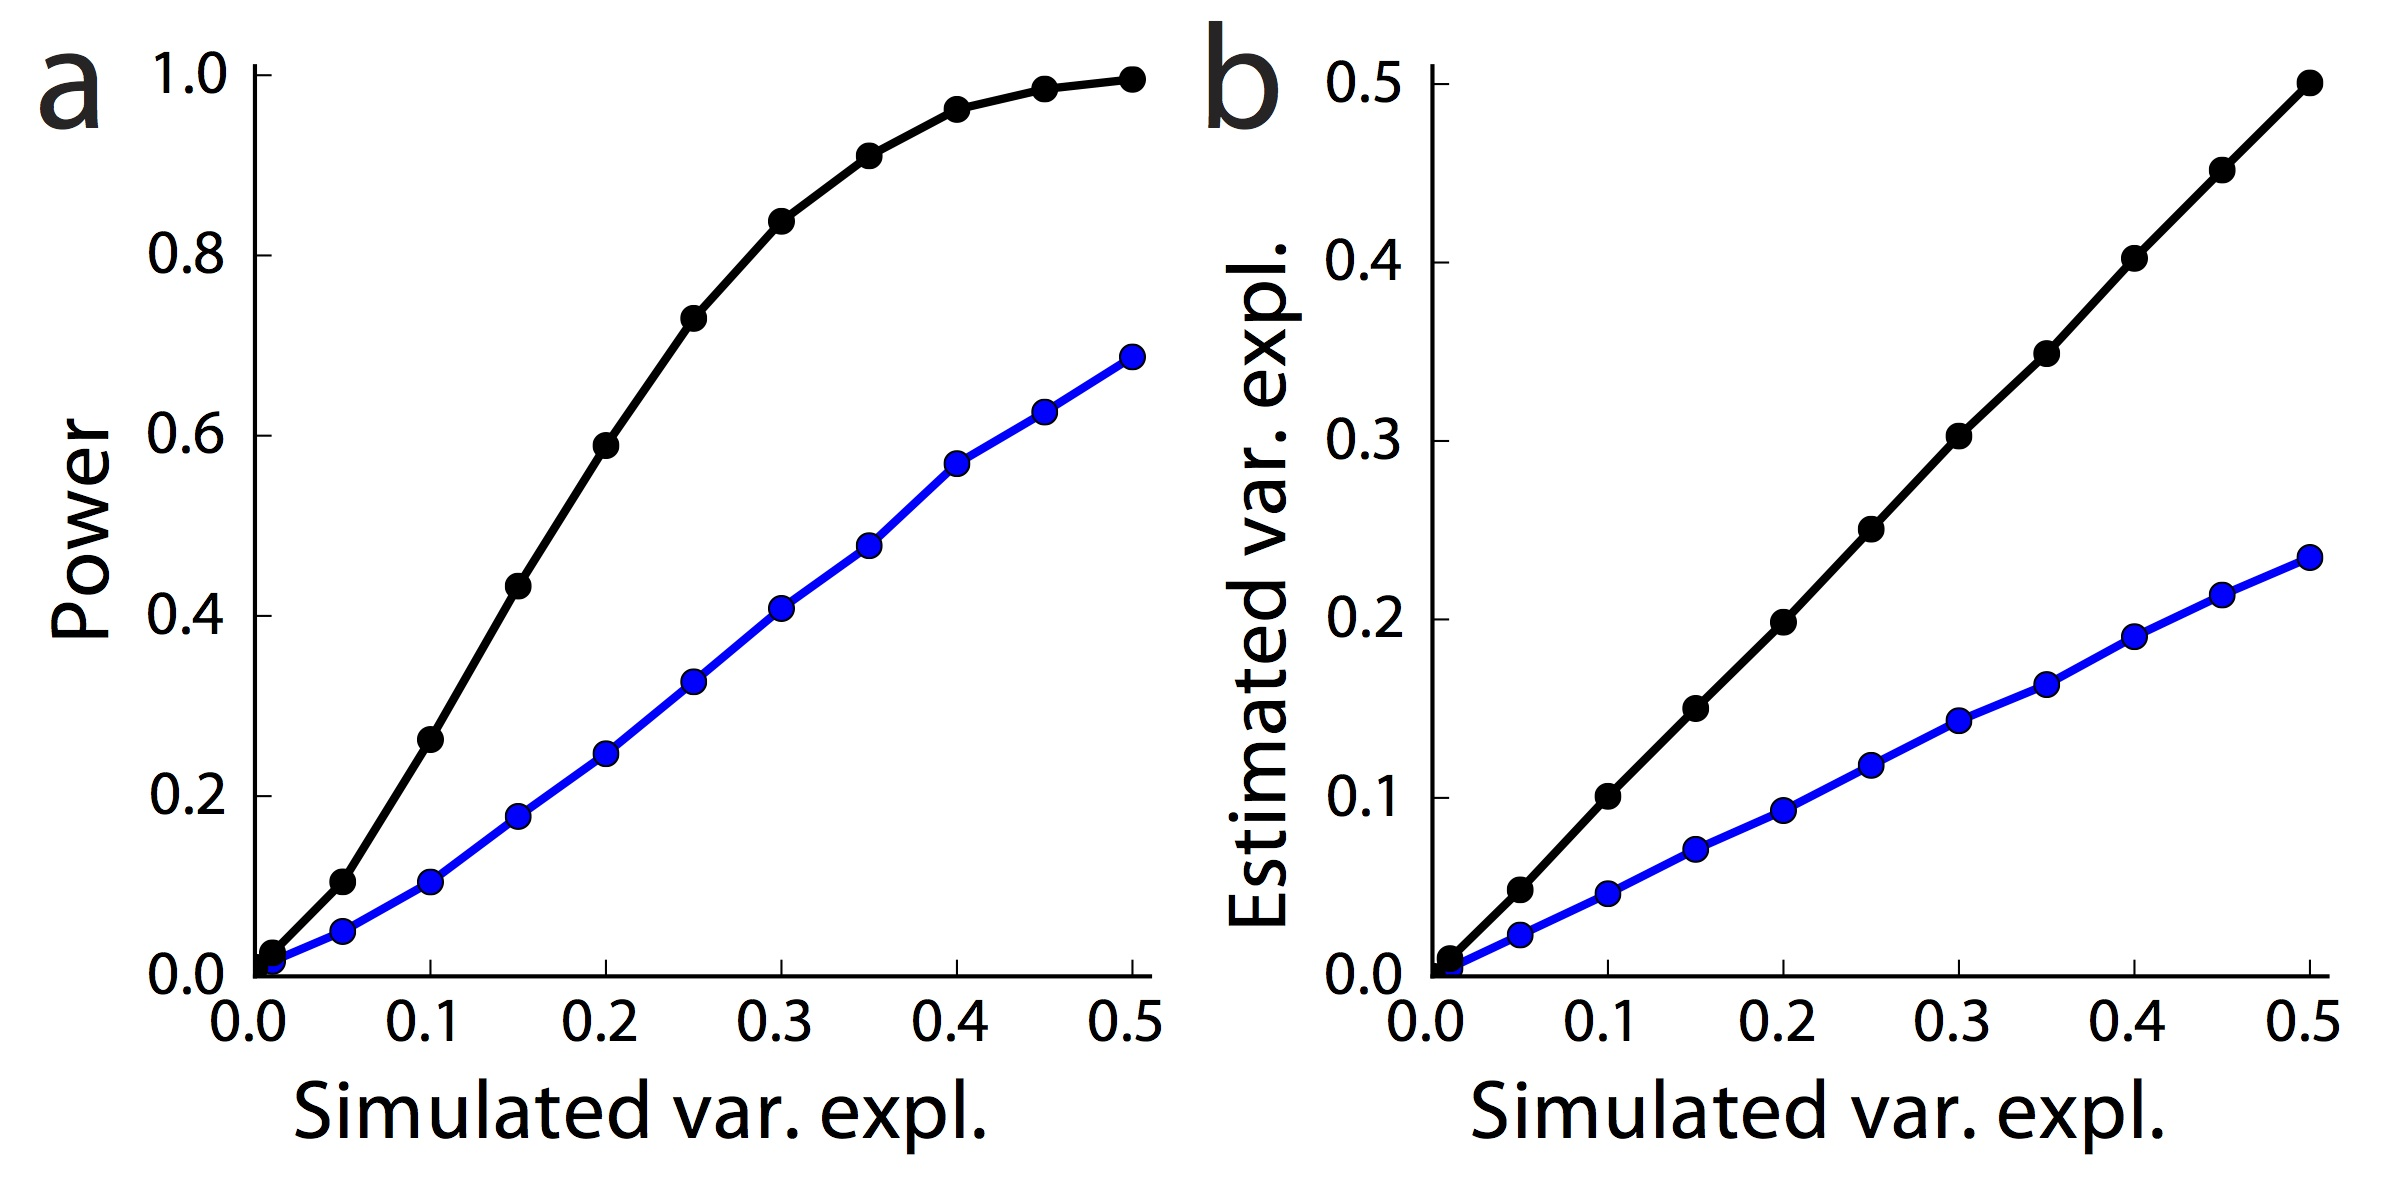
\includegraphics[width=0.7\textwidth]{Figures/Chapter4/SuppFig1.jpg}
\end{figure}

\textbf{STR genotyping errors reduce power to detect eSTR associations}. \textbf{a}. Power to detect associations and \textbf{b}. estimated variance explained for different simulated values of variance explained by the STR. (black: observed capillary electrophoresis genotypes, blue: lobSTR genotypes).

\pagebreak
\subsection{Supplementary Figure 2}
\begin{figure}[h!]
\centering
\label{fig:estrsupfig2}
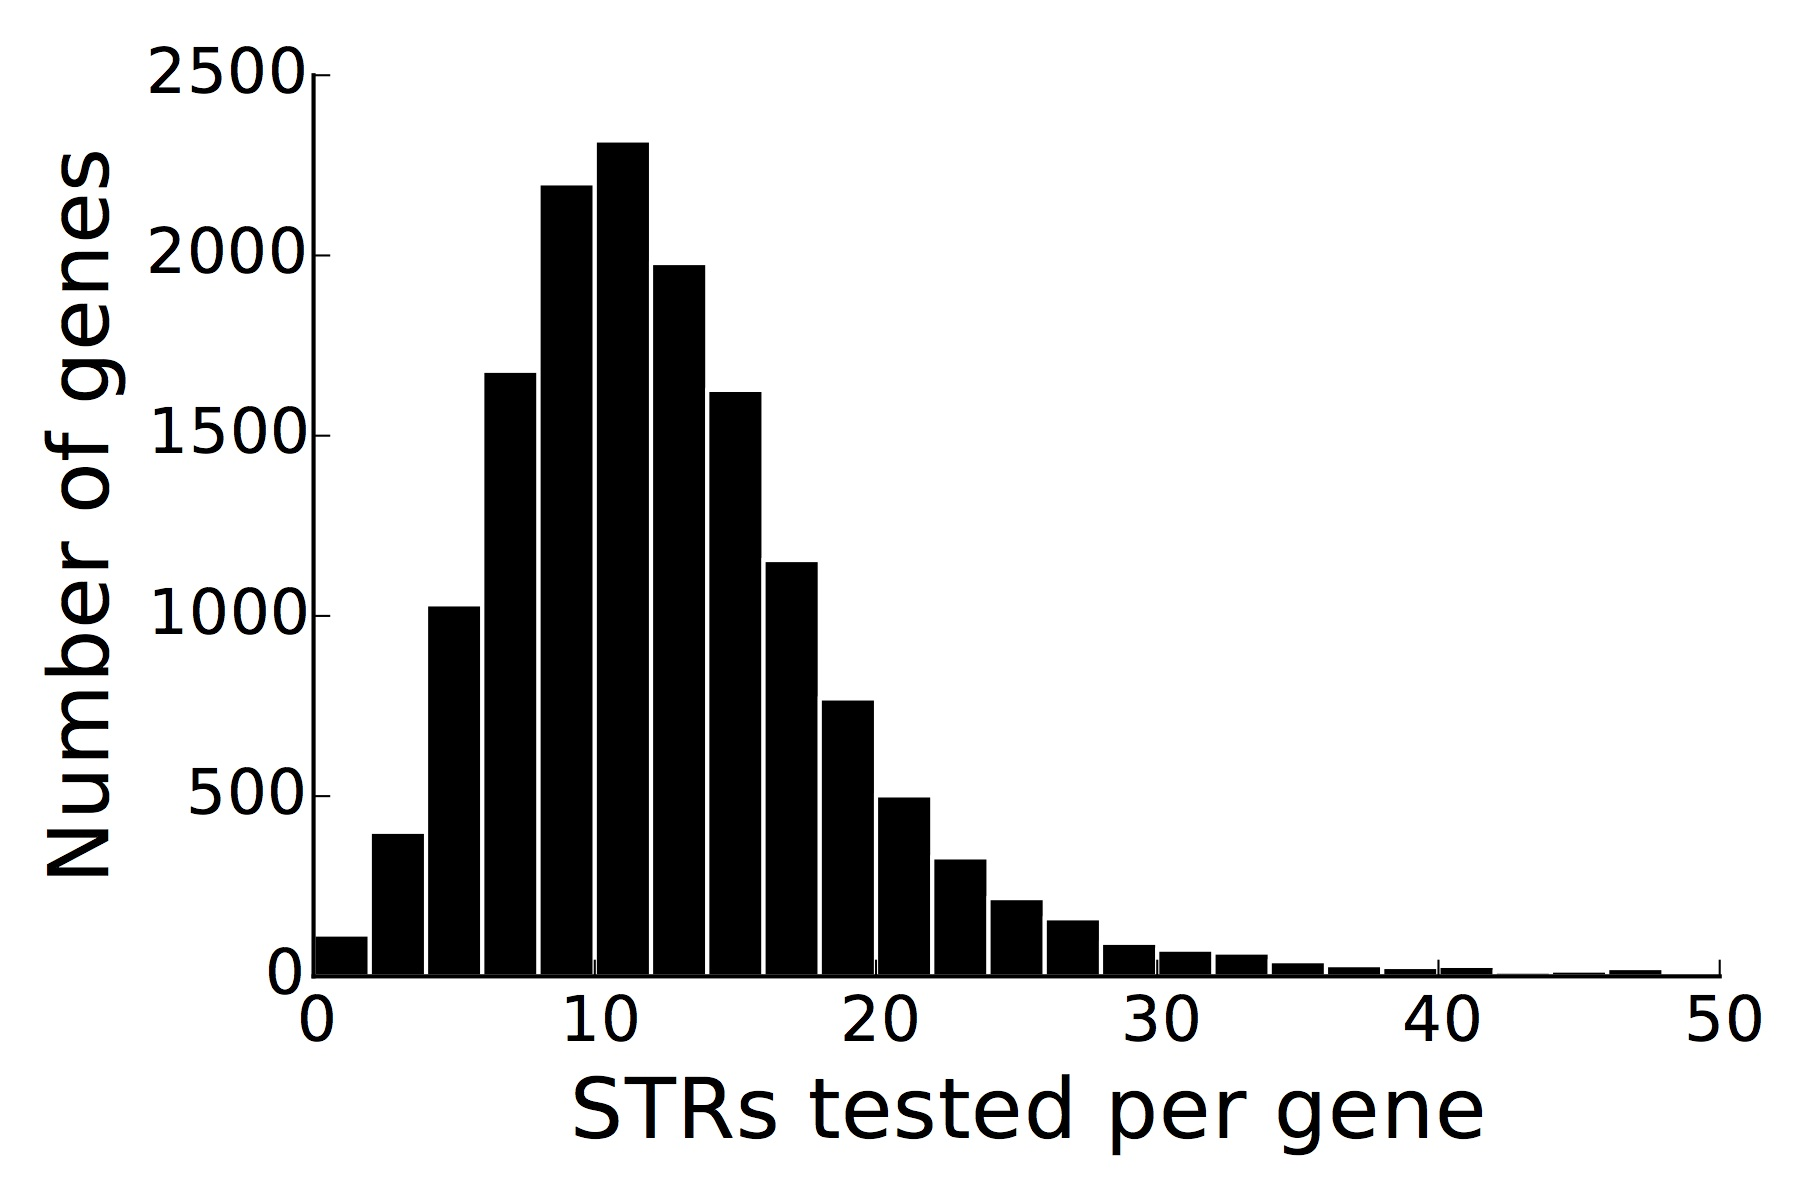
\includegraphics[width=0.5\textwidth]{Figures/Chapter4/SuppFig2.jpg}
\end{figure}

\textbf{Number of STRs tested per gene.} Histogram gives the number of STRs within 100kb of each gene that passed quality filters and were included in the eSTR analysis.

\pagebreak
\subsection{Supplementary Figure 3}
\begin{figure}[h!]
\centering
\label{fig:estrsupfig3}
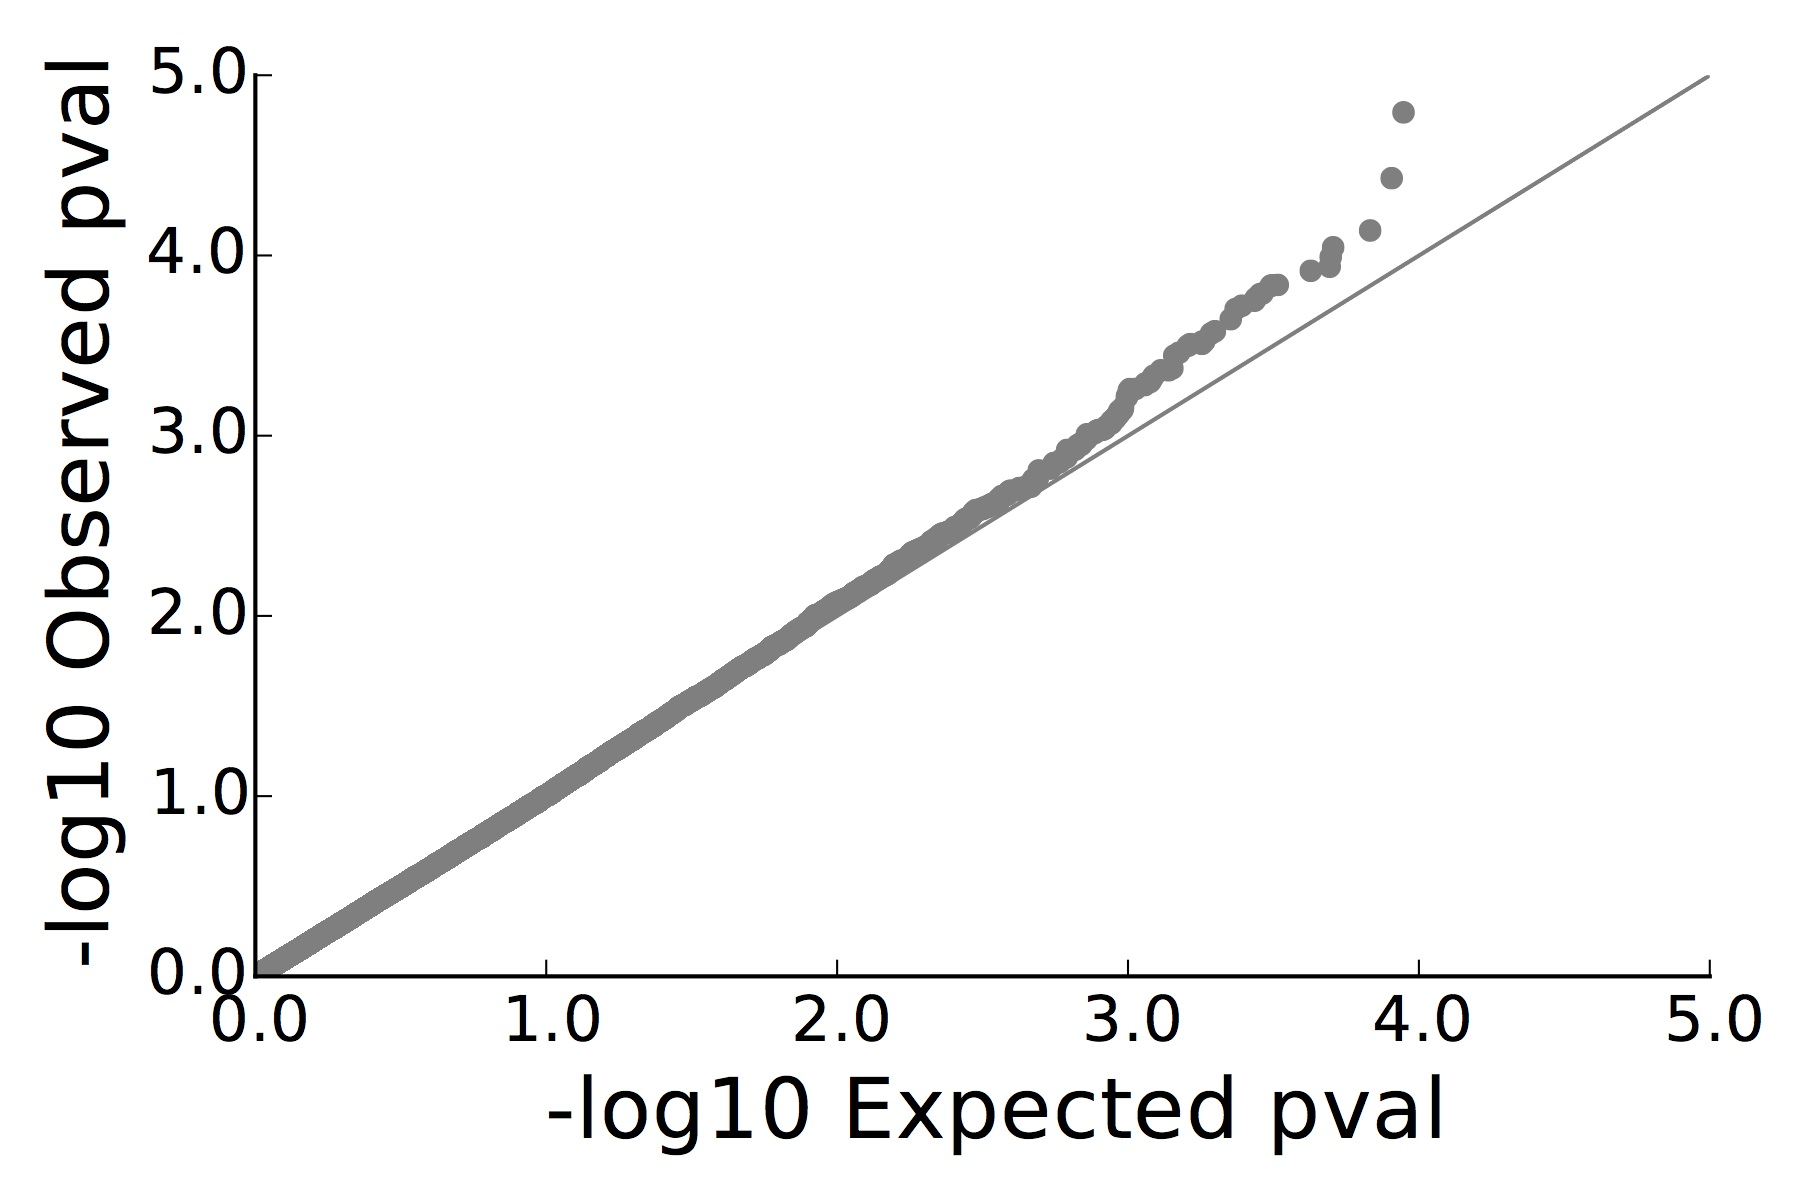
\includegraphics[width=0.5\textwidth]{Figures/Chapter4/SuppFig3.jpg}
\end{figure}

\textbf{Unlinked controls follow the null}. QQ plot of association tests between random unlinked STRs and genes.

\pagebreak
\subsection{Supplementary Figure 4}
\begin{figure}[h!]
\centering
\label{fig:estrsupfig4}
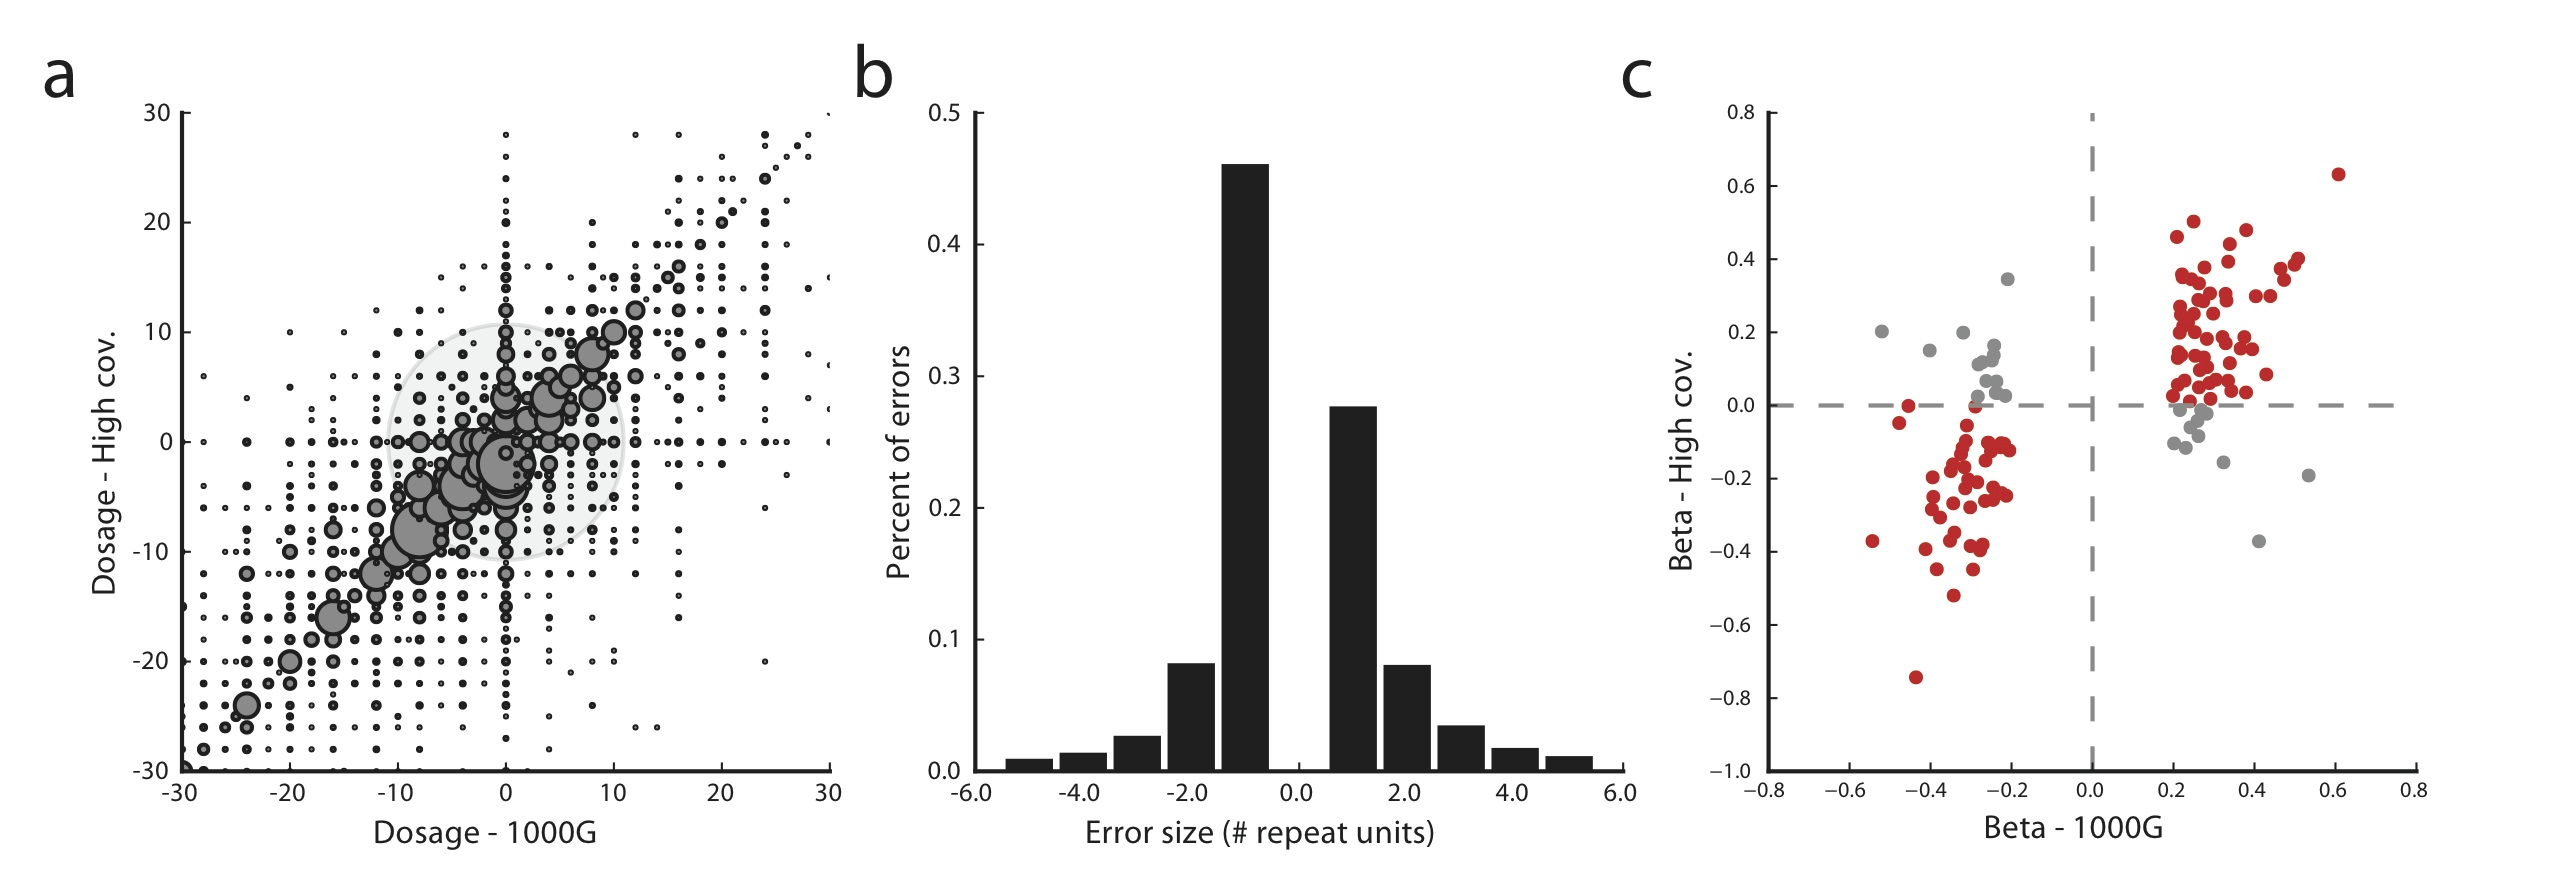
\includegraphics[width=0.9\textwidth]{Figures/Chapter4/SuppFig4.jpg}
\end{figure}

\textbf{Validation of eSTR analysis using high coverage genotype calls}. \textbf{a}. Comparison of STR dosage in low coverage 1000 Genomes calls vs. calls from high coverage targeted sequencing of promoter STRs. Bubble area represents the number of calls at each data point. For reference, the bubble at -20,-20 represents 176 calls. 0 denotes the reference allele. The transparent bubble in the center represents calls that are homozygous reference in both datasets. \textbf{b}. Distribution of the size of errors for discordant allele calls. The majority of errors (89.4\%) are off by one or two repeat units. \textbf{c}. Comparison of eSTR effect sizes between the low and high coverage datasets. Red dots denote eSTRs with concordant effect directions.

\pagebreak
\subsection{Supplementary Figure 5}
\begin{figure}[h!]
\centering
\label{fig:estrsupfig5}
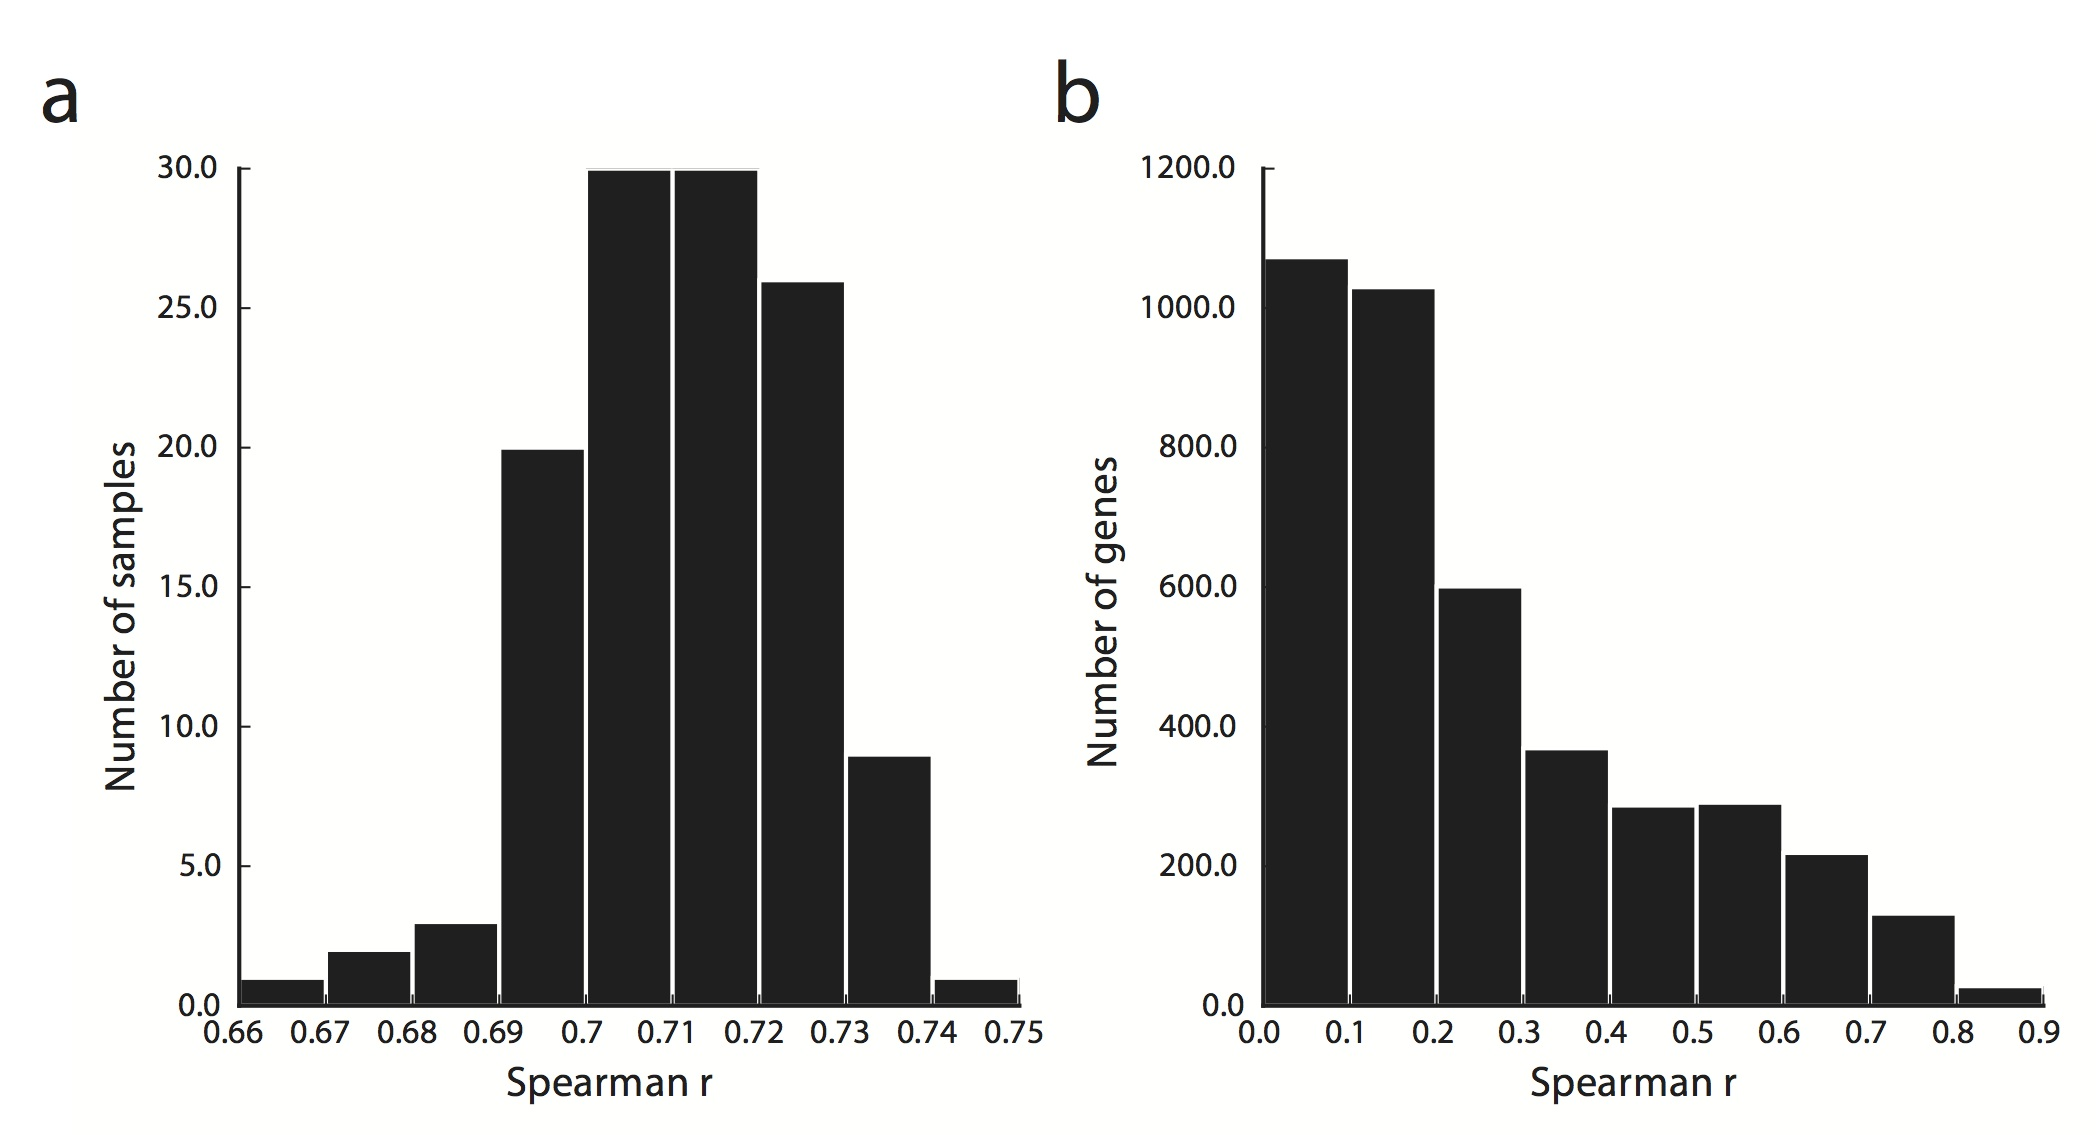
\includegraphics[width=0.7\textwidth]{Figures/Chapter4/SuppFig5.jpg}
\end{figure}

\textbf{Expression values are moderately reproducible across platforms.} \textbf{a}. Distribution of Spearman rank correlation coefficients between gene expression profiles of individuals measured on microarray vs. RNA-sequencing platforms. \textbf{b}. Distribution of Spearman rank correlation coefficients between the order of individuals ranked by expression levels across transcripts measured using microarray vs. RNA-sequencing platforms.

\pagebreak
\subsection{Supplementary Figure 6}
\begin{figure}[h!]
\centering
\label{fig:estrsupfig6}
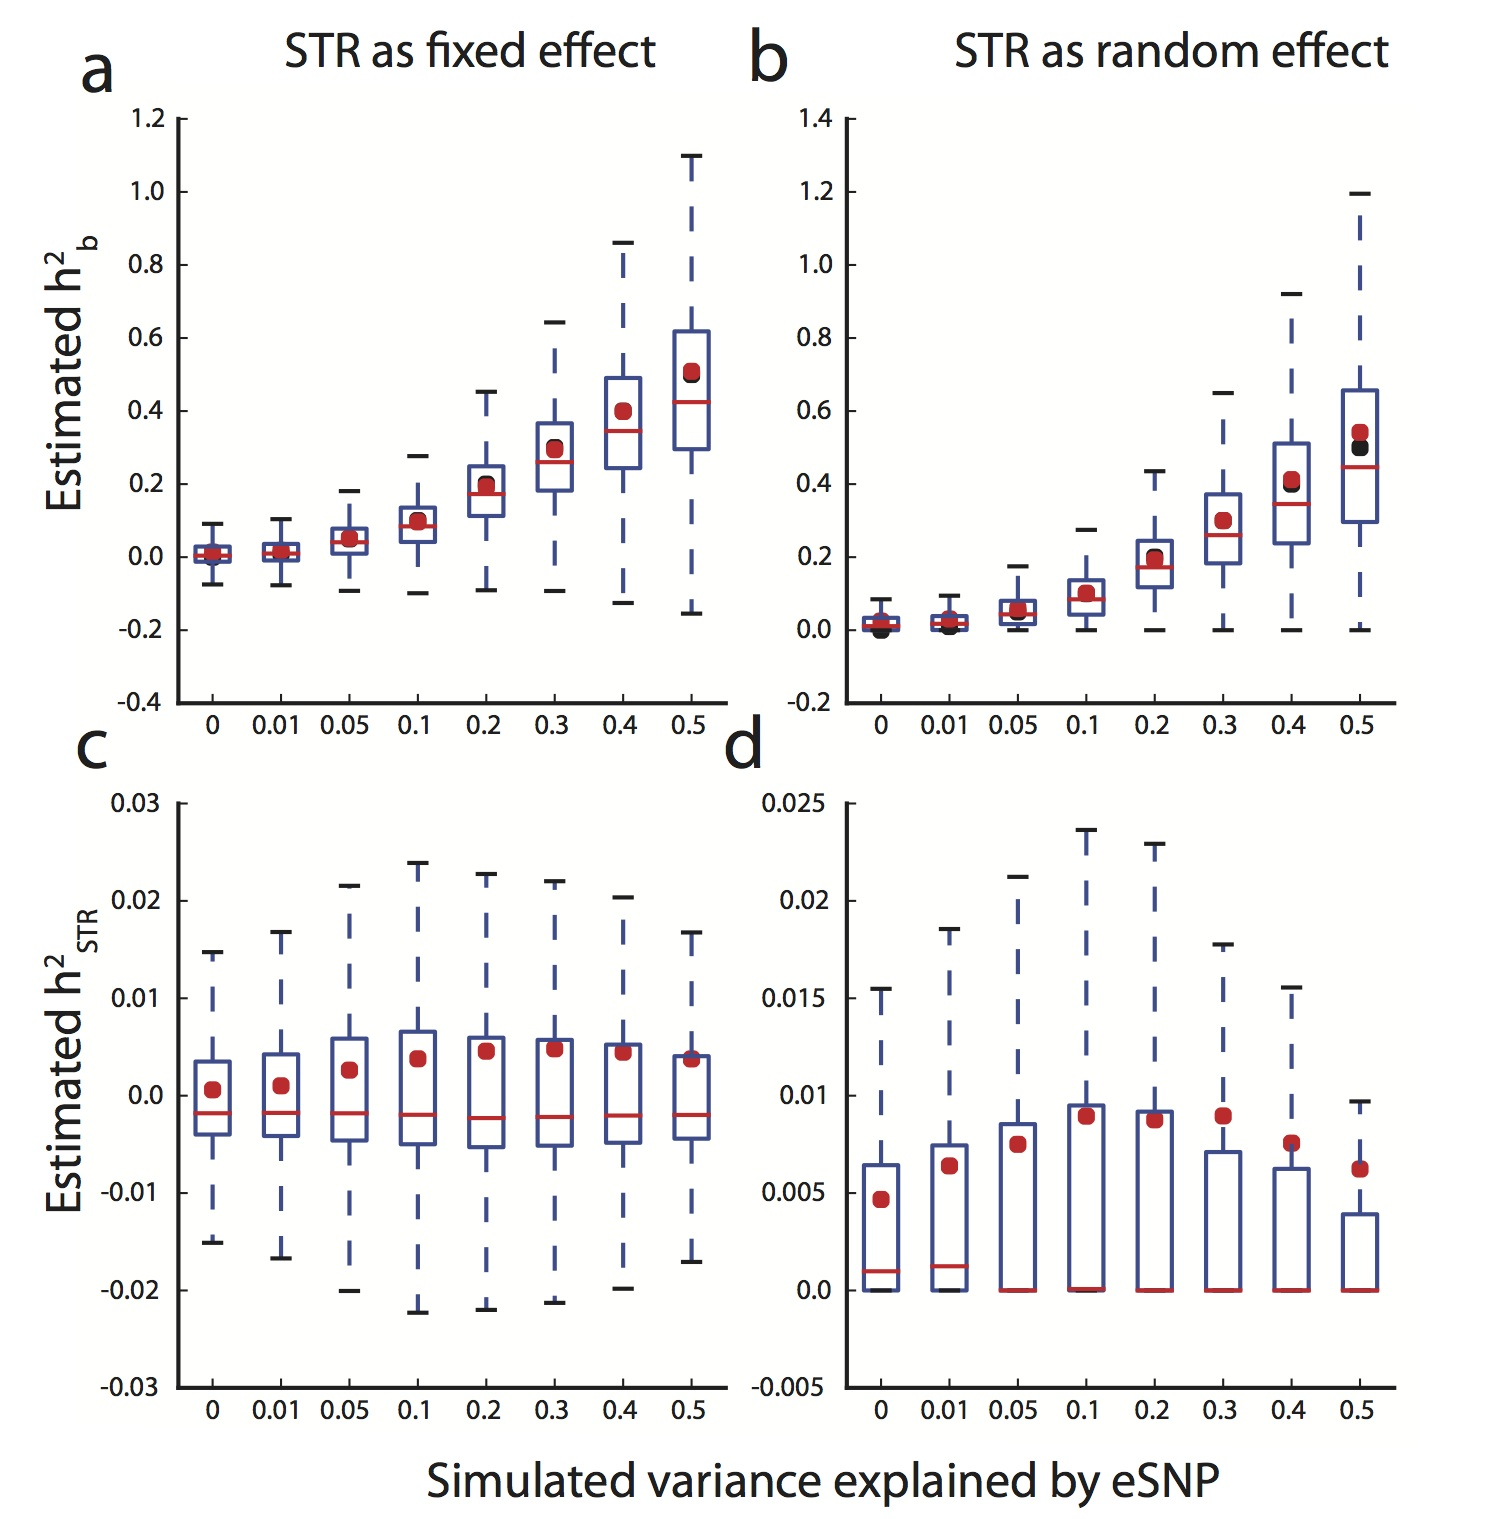
\includegraphics[width=0.7\textwidth]{Figures/Chapter4/SuppFig6.jpg}
\end{figure}
\textbf{Variance partitioning simulations with a single causal SNP} Plots show variance partitioning results from simulations in which each gene has a single causal eSNP.
(\textbf{a}\&\textbf{b}) The distributions of $h^2_{b}$
(\textbf{c}\&\textbf{d}) The distributions of $h^2_{STR}$
(\textbf{a}\&\textbf{c}) The LMM simulations with STRs as fixed effects
(\textbf{b}\&\textbf{d}) The LMM simulations with STRs as random effects
(\textbf{a}-\textbf{d}) Black points denote the true value of the variance explained by the causal SNP. 
Red dots denote the average value of the estimator.
Red bars denote the median value of the estimator.
The figure shows that the median values of the lead STRs are largely insensitive to the presence of a strong SNP eQTL.

\pagebreak
\subsection{Supplementary Figure 7}
\begin{figure}[h!]
\centering
\label{fig:estrsupfig7}
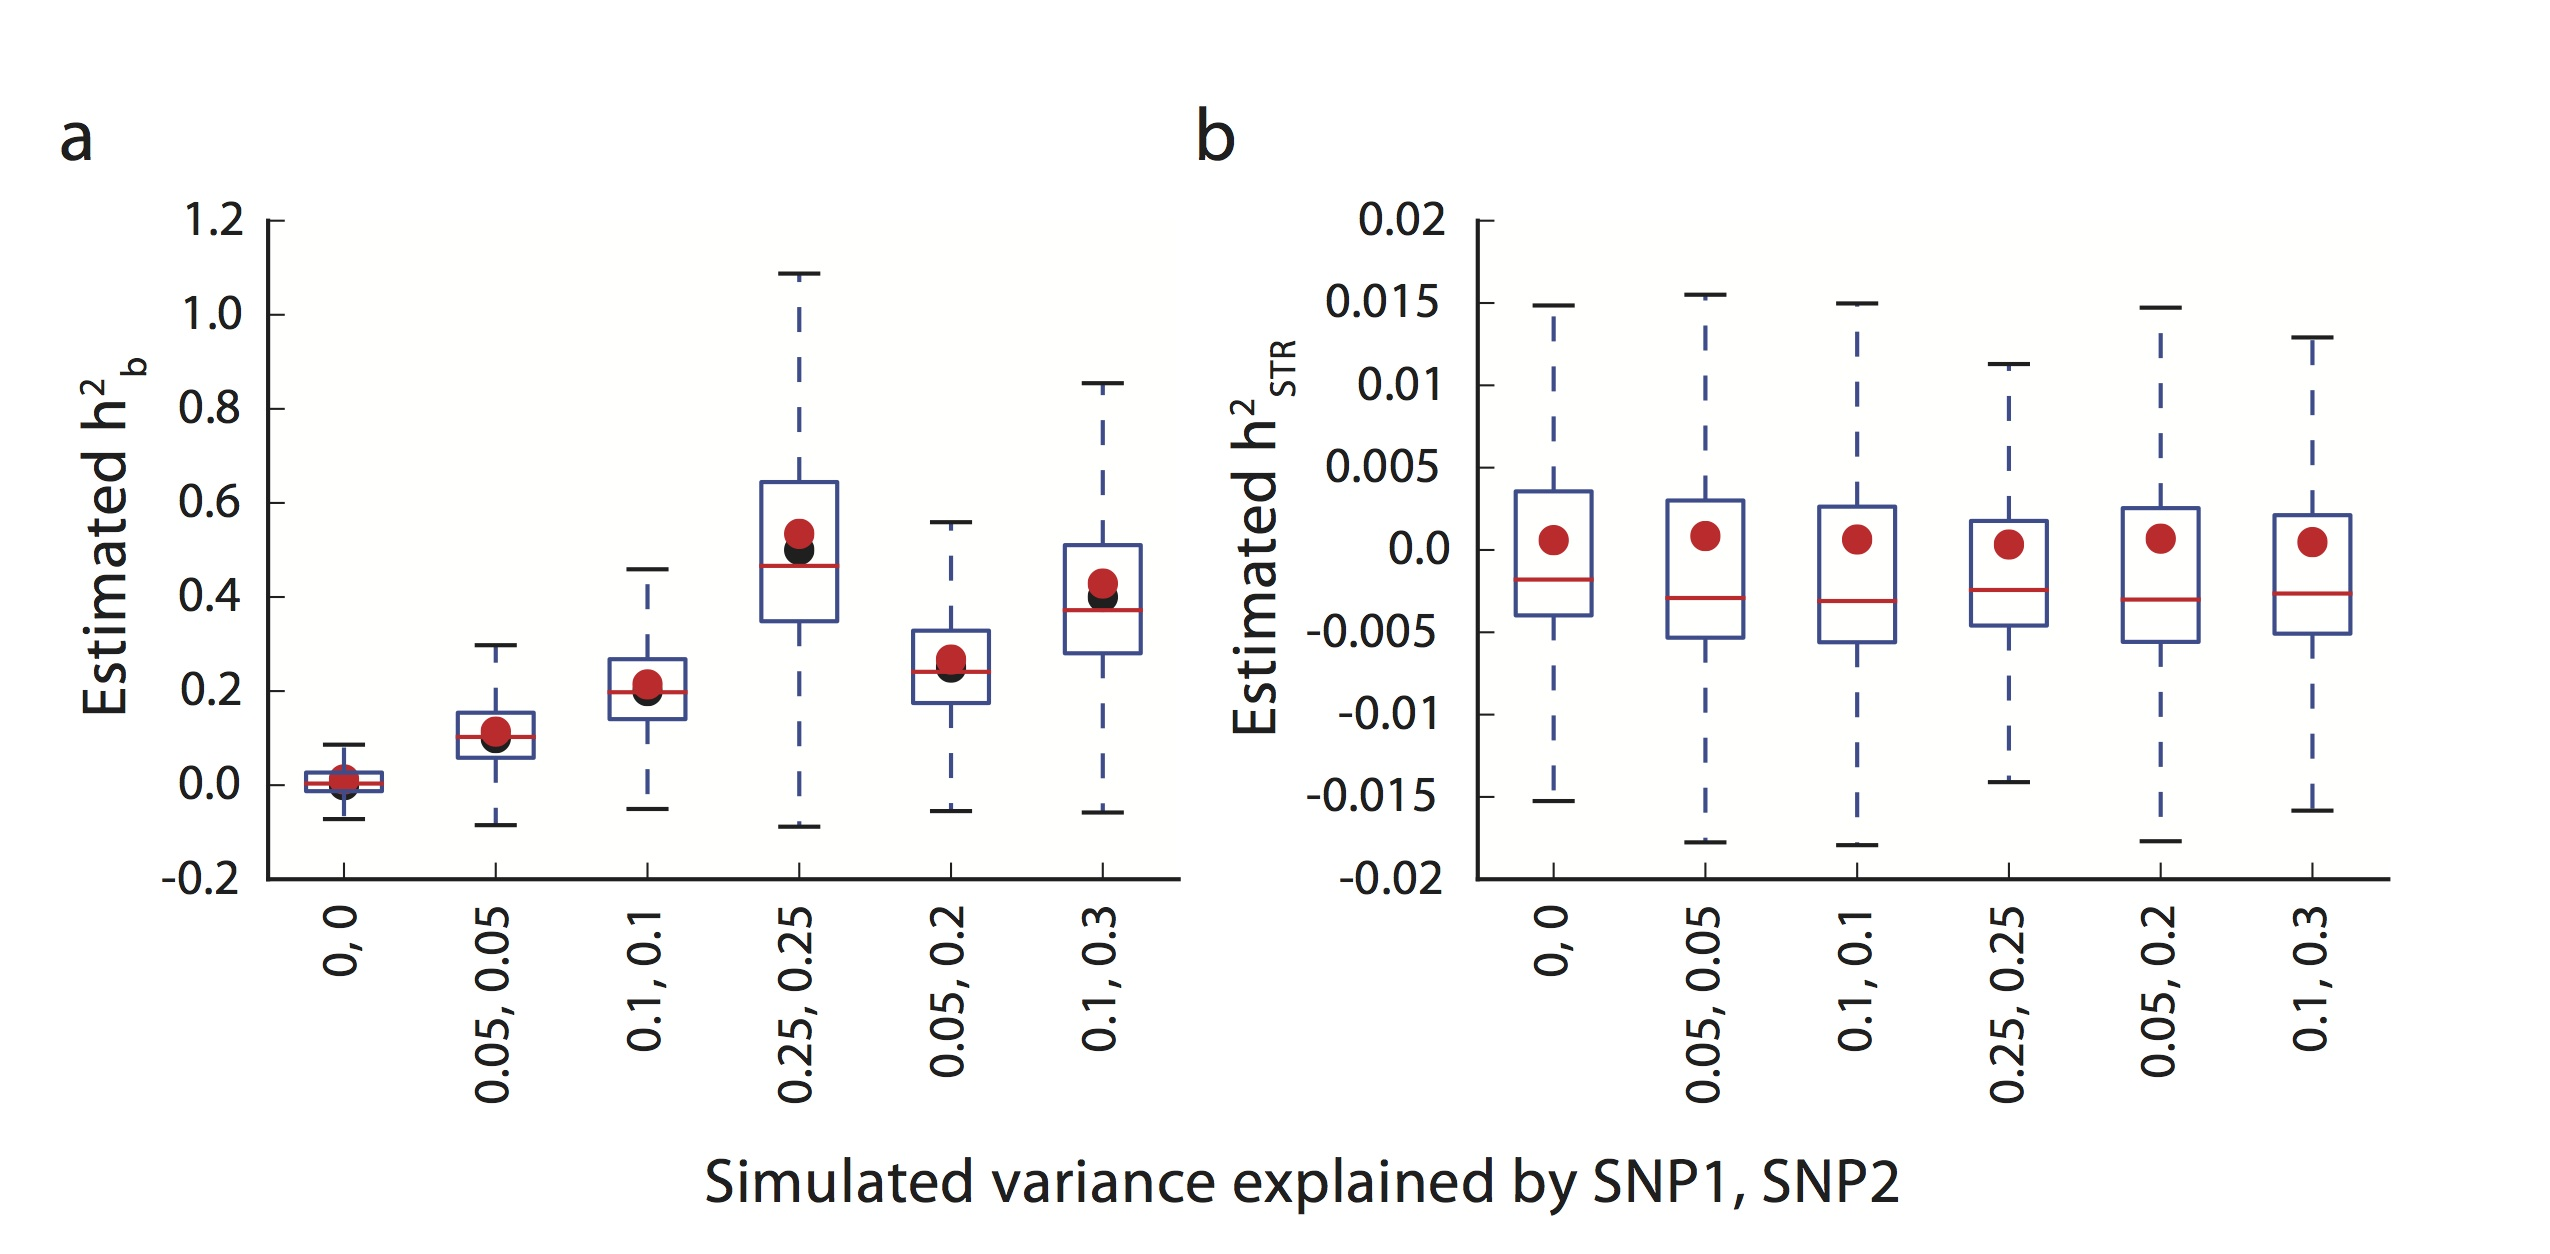
\includegraphics[width=0.7\textwidth]{Figures/Chapter4/SuppFig7.jpg}
\end{figure}
\textbf{Variance partitioning simulations with two causal SNPs} Plots show variance partitioning results from simulations in which each gene has two causal eSNPs. \textbf{a} The distributions of $h^2_{b}$. \textbf{b} The distributions of $h^2_{STR}$. Black points denote the true value of the variance explained by the causal SNPs. 
Red dots denote the average value of the estimator.
Red bars denote the median value of the estimator.

\pagebreak
\subsection{Supplementary Figure 8}
\begin{figure}[h!]
\centering
\label{fig:estrsupfig8}
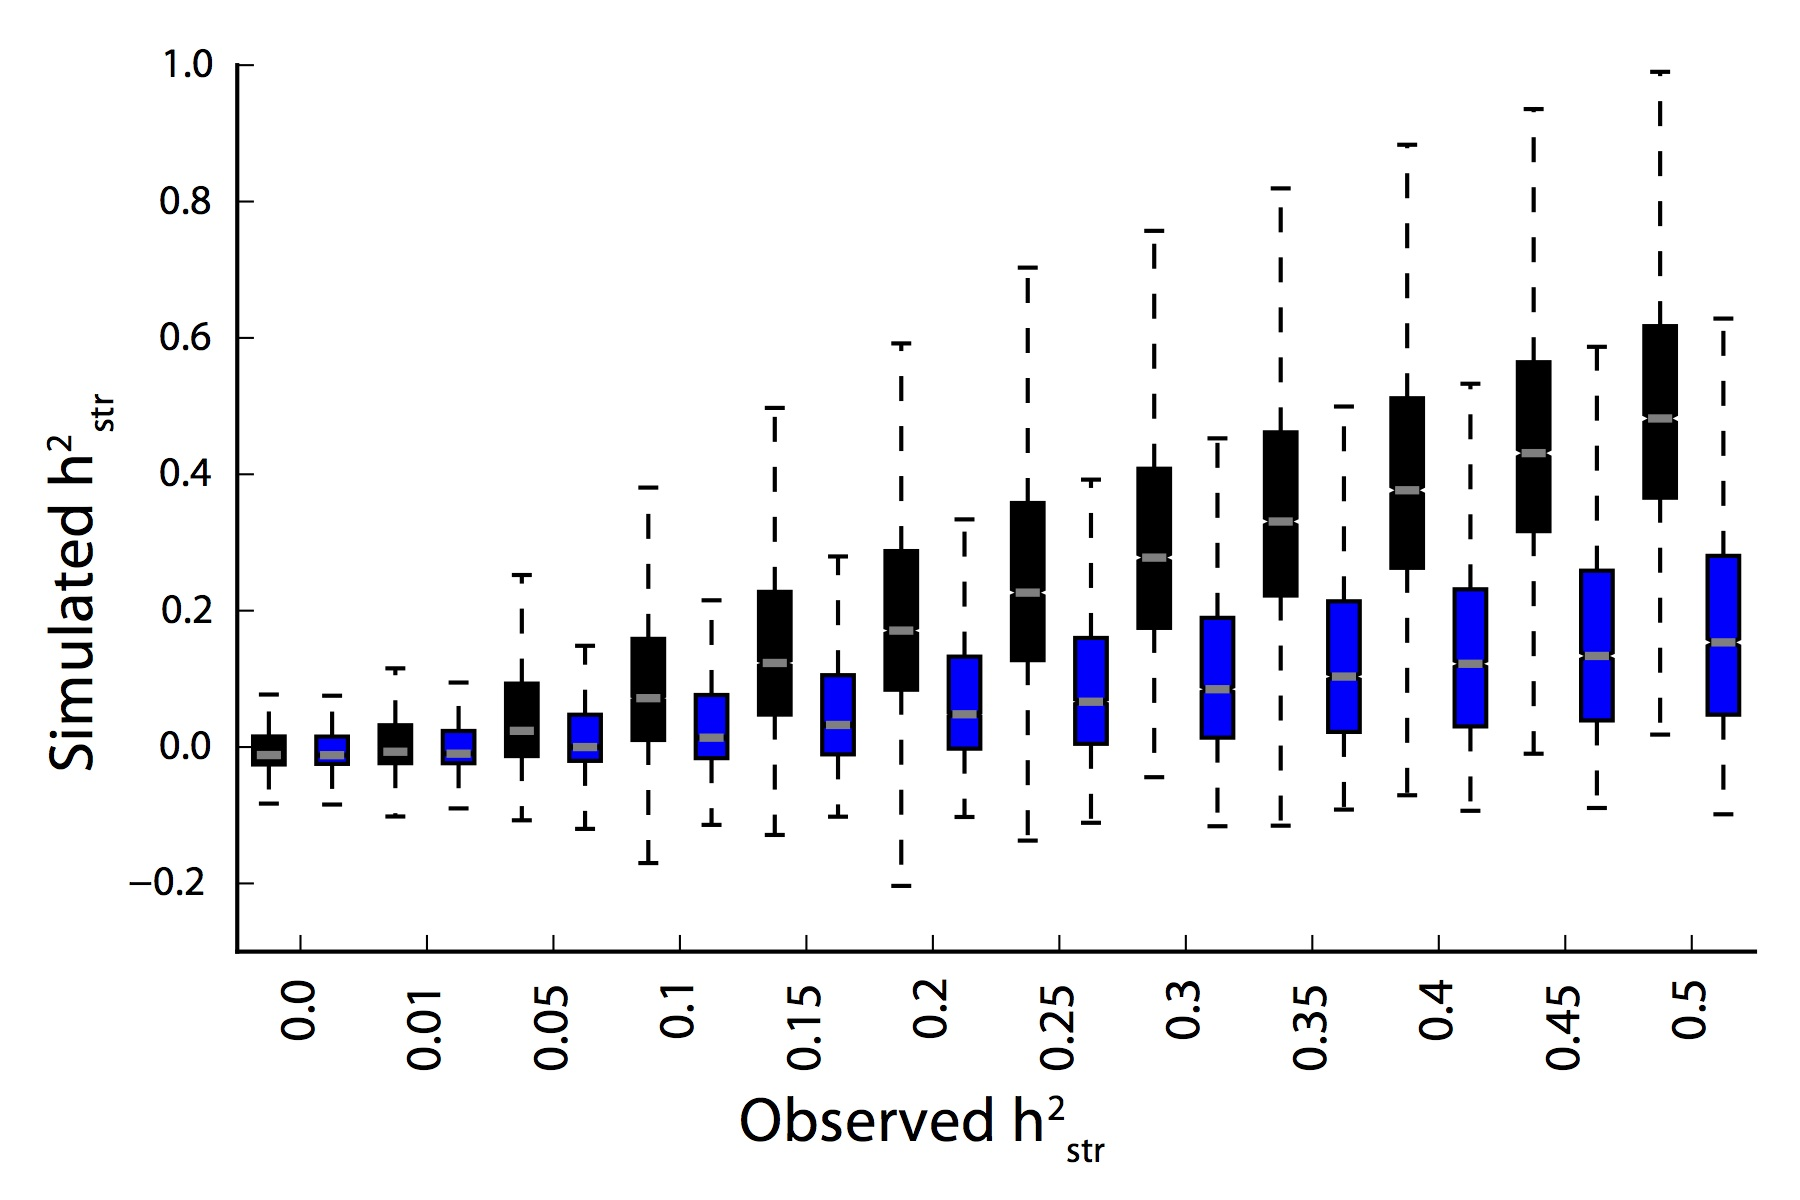
\includegraphics[width=0.7\textwidth]{Figures/Chapter4/SuppFig8.jpg}
\end{figure}

\textbf{STR genotype errors cause underestimation of $h^2_{STR}$}. The distribution of observed $h^2_{STR}$ for each simulated value of $h^2_{STR}$ is shown for an LMM analysis conducted using true genotypes (black) vs. observed genotypes (blue). In the presence of genotyping errors, $h^2_{STR}$ is strongly underestimated.

\pagebreak
\subsection{Supplementary Figure 9}
\begin{figure}[h!]
\centering
\label{fig:estrsupfig9}
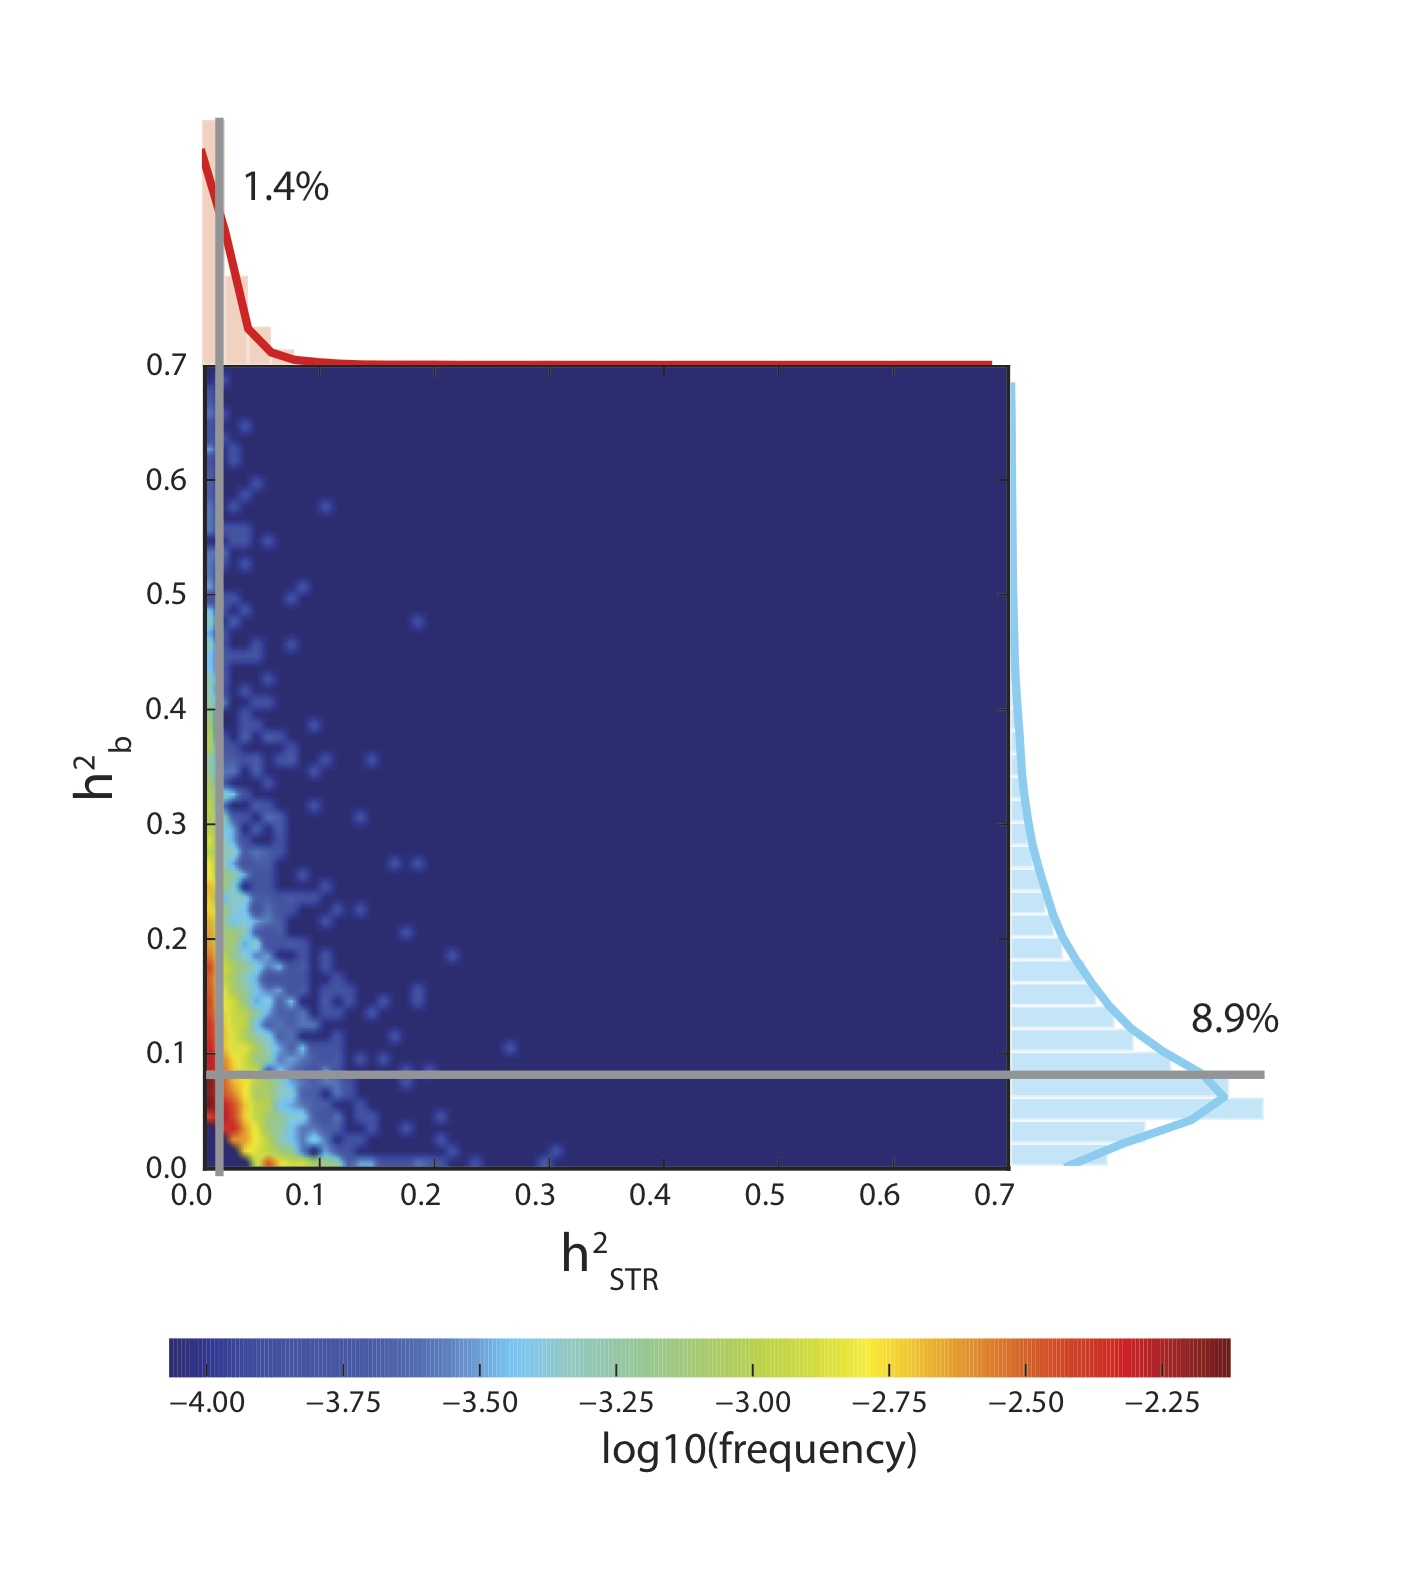
\includegraphics[width=0.7\textwidth]{Figures/Chapter4/SuppFig9.jpg}
\end{figure}
\textbf{Partitioning variance when treaing the STR as a random effect.} The heatmap shows the distribution of $h^2_{STR}$ and $h^2_{b}$ for each gene. Dashed gray lines give the medians of each distribution.

\pagebreak
\subsection{Supplementary Figure 10}
\begin{figure}[h!]
\centering
\label{fig:estrsupfig10}
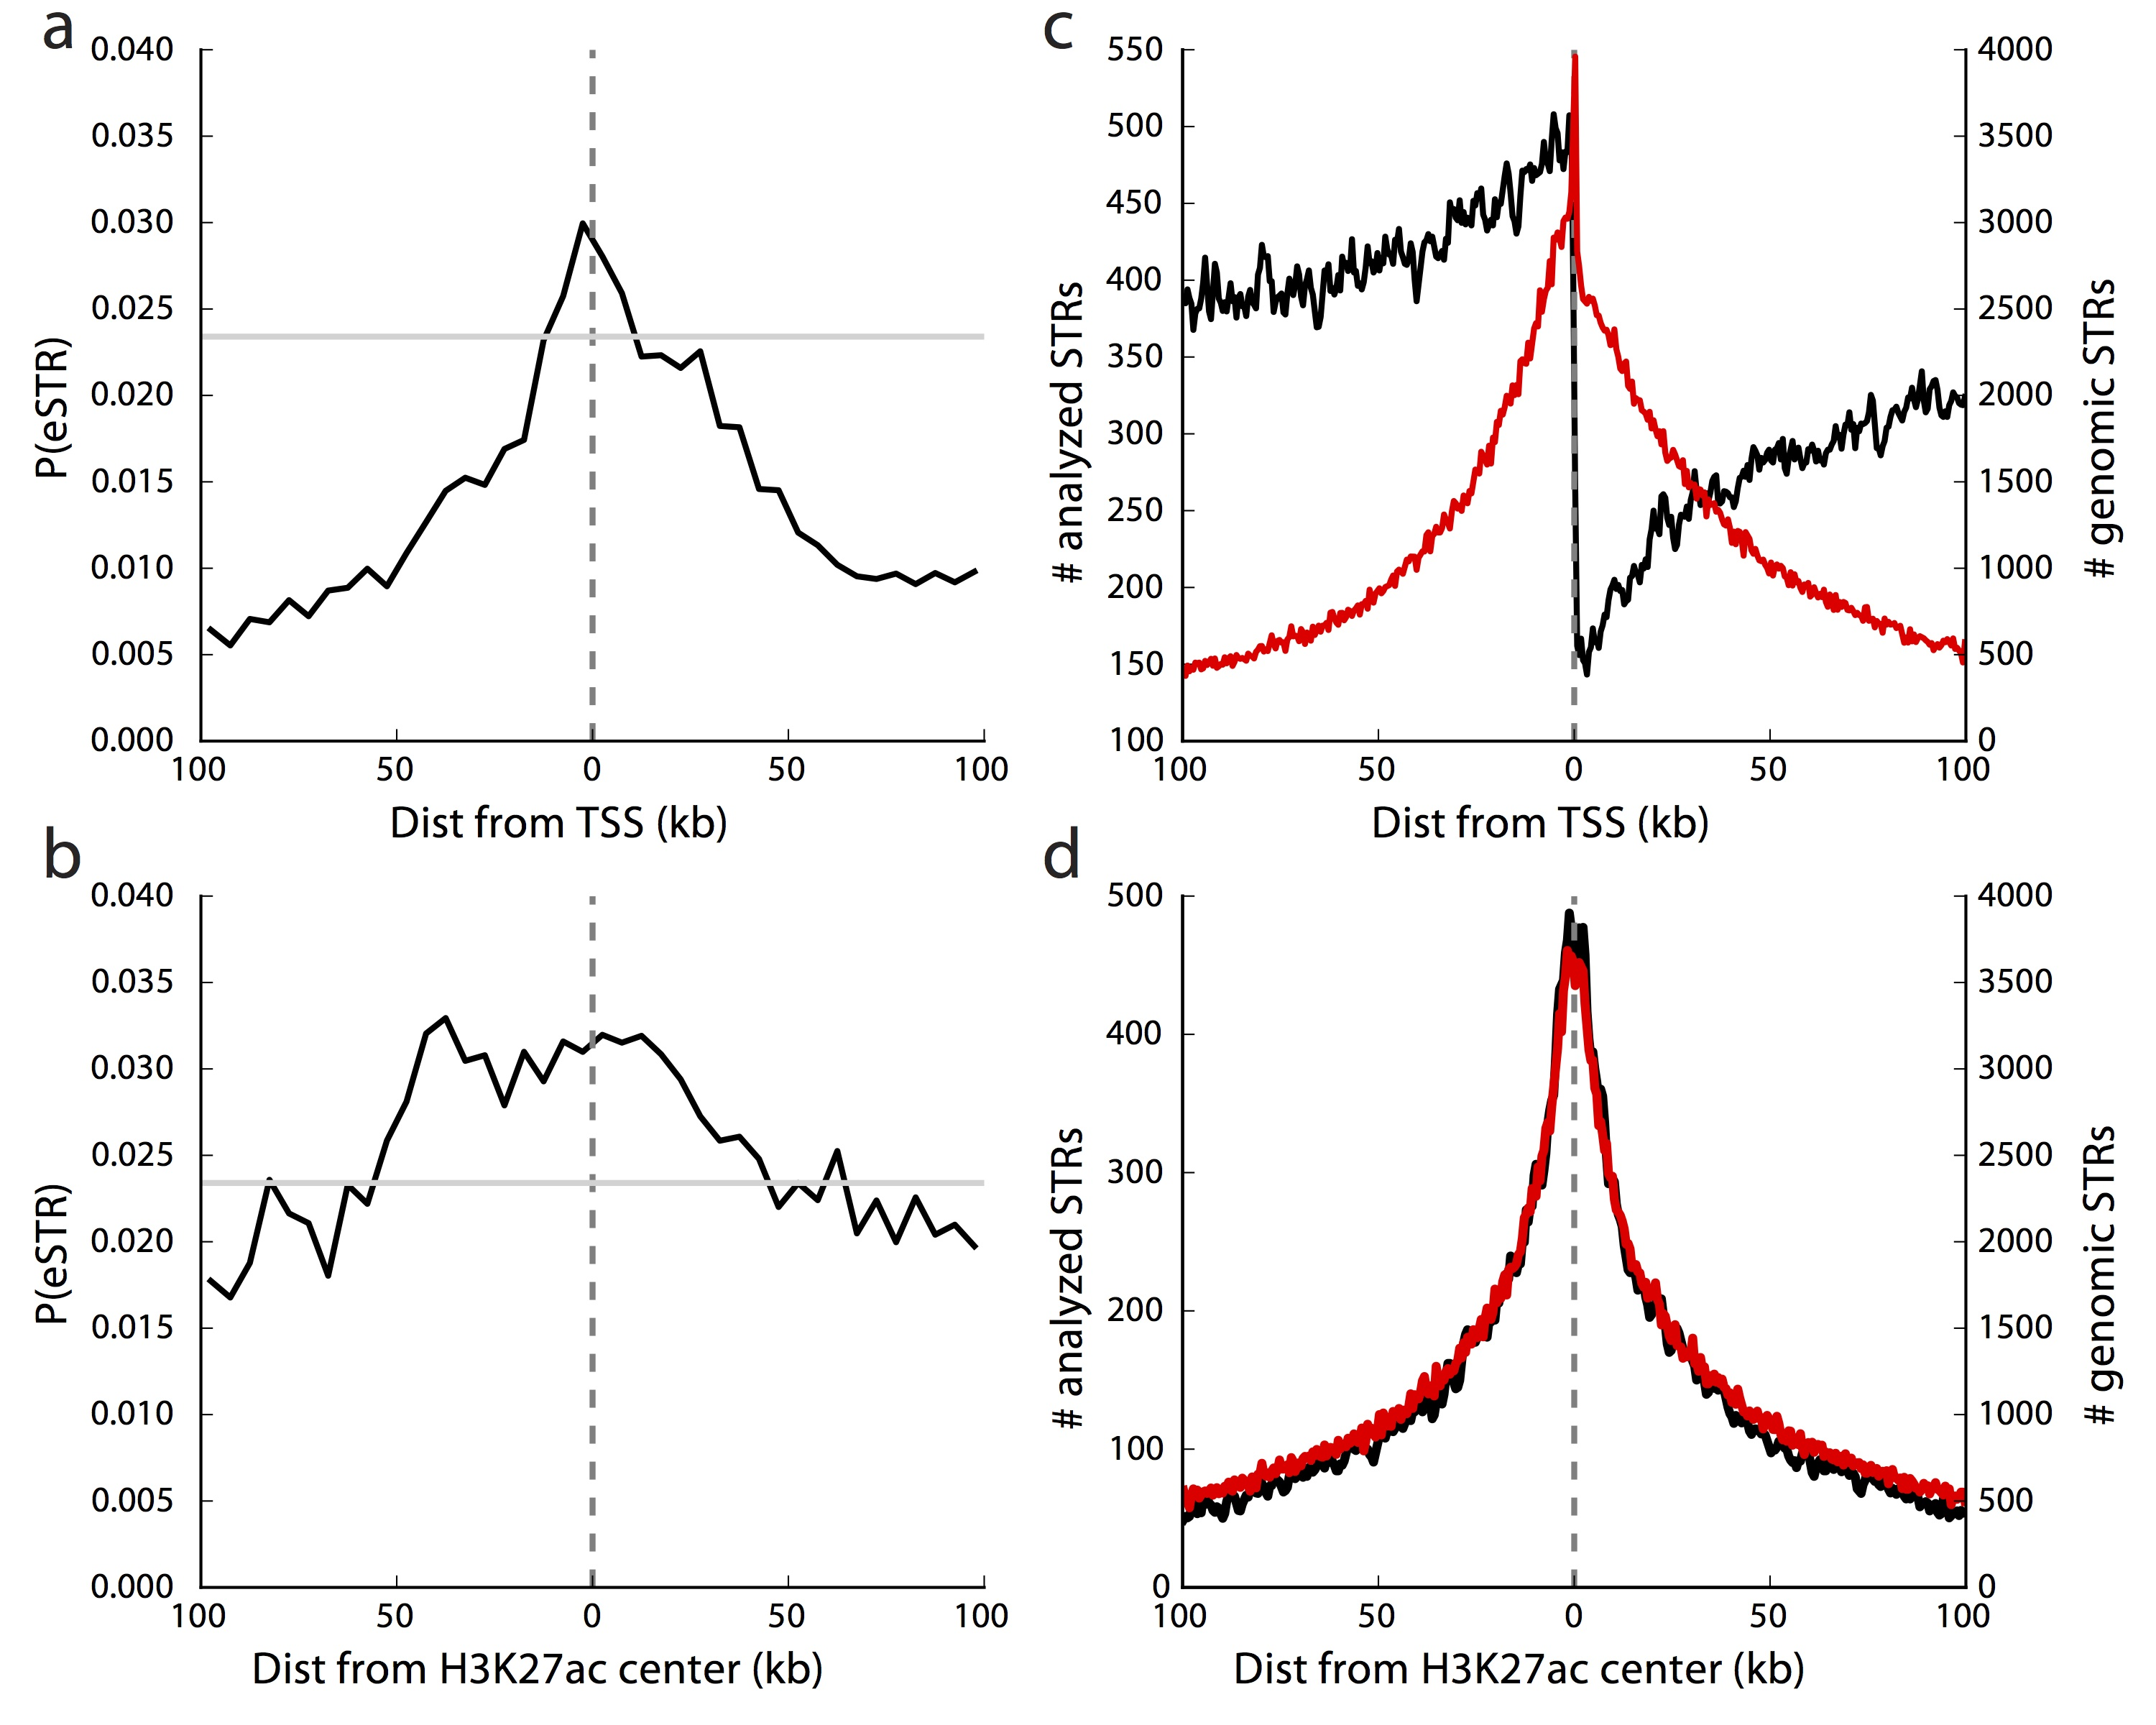
\includegraphics[width=0.7\textwidth]{Figures/Chapter4/SuppFig10.jpg}
\end{figure}
\textbf{Enrichment of eSTRs at promoters and enhancers}. For each distance bin around (\textbf{a}) the TSS (\textbf{b}) center of H3K27ac peaks, the plot shows the percentage of STRs that were analyzed in that bin that were called as significant eSTRs. \textbf{c} and \textbf{d} show the number of STRs in each distance bin. Black lines show the number of STRs that were included in our analysis (meaning they showed sufficient variability and are near genes). Red lines show the number of all STRs in the genome in each bin. Black lines were smoothed by averaging sliding windows of 3 consecutive data points. \textbf{a} and 
\textbf{b} were binned by 10kb. \textbf{c} and \textbf{d} were binned by 500bp.

\pagebreak
\subsection{Supplementary Figure 11}
\begin{figure}[h!]
\centering
\label{fig:estrsupfig11}
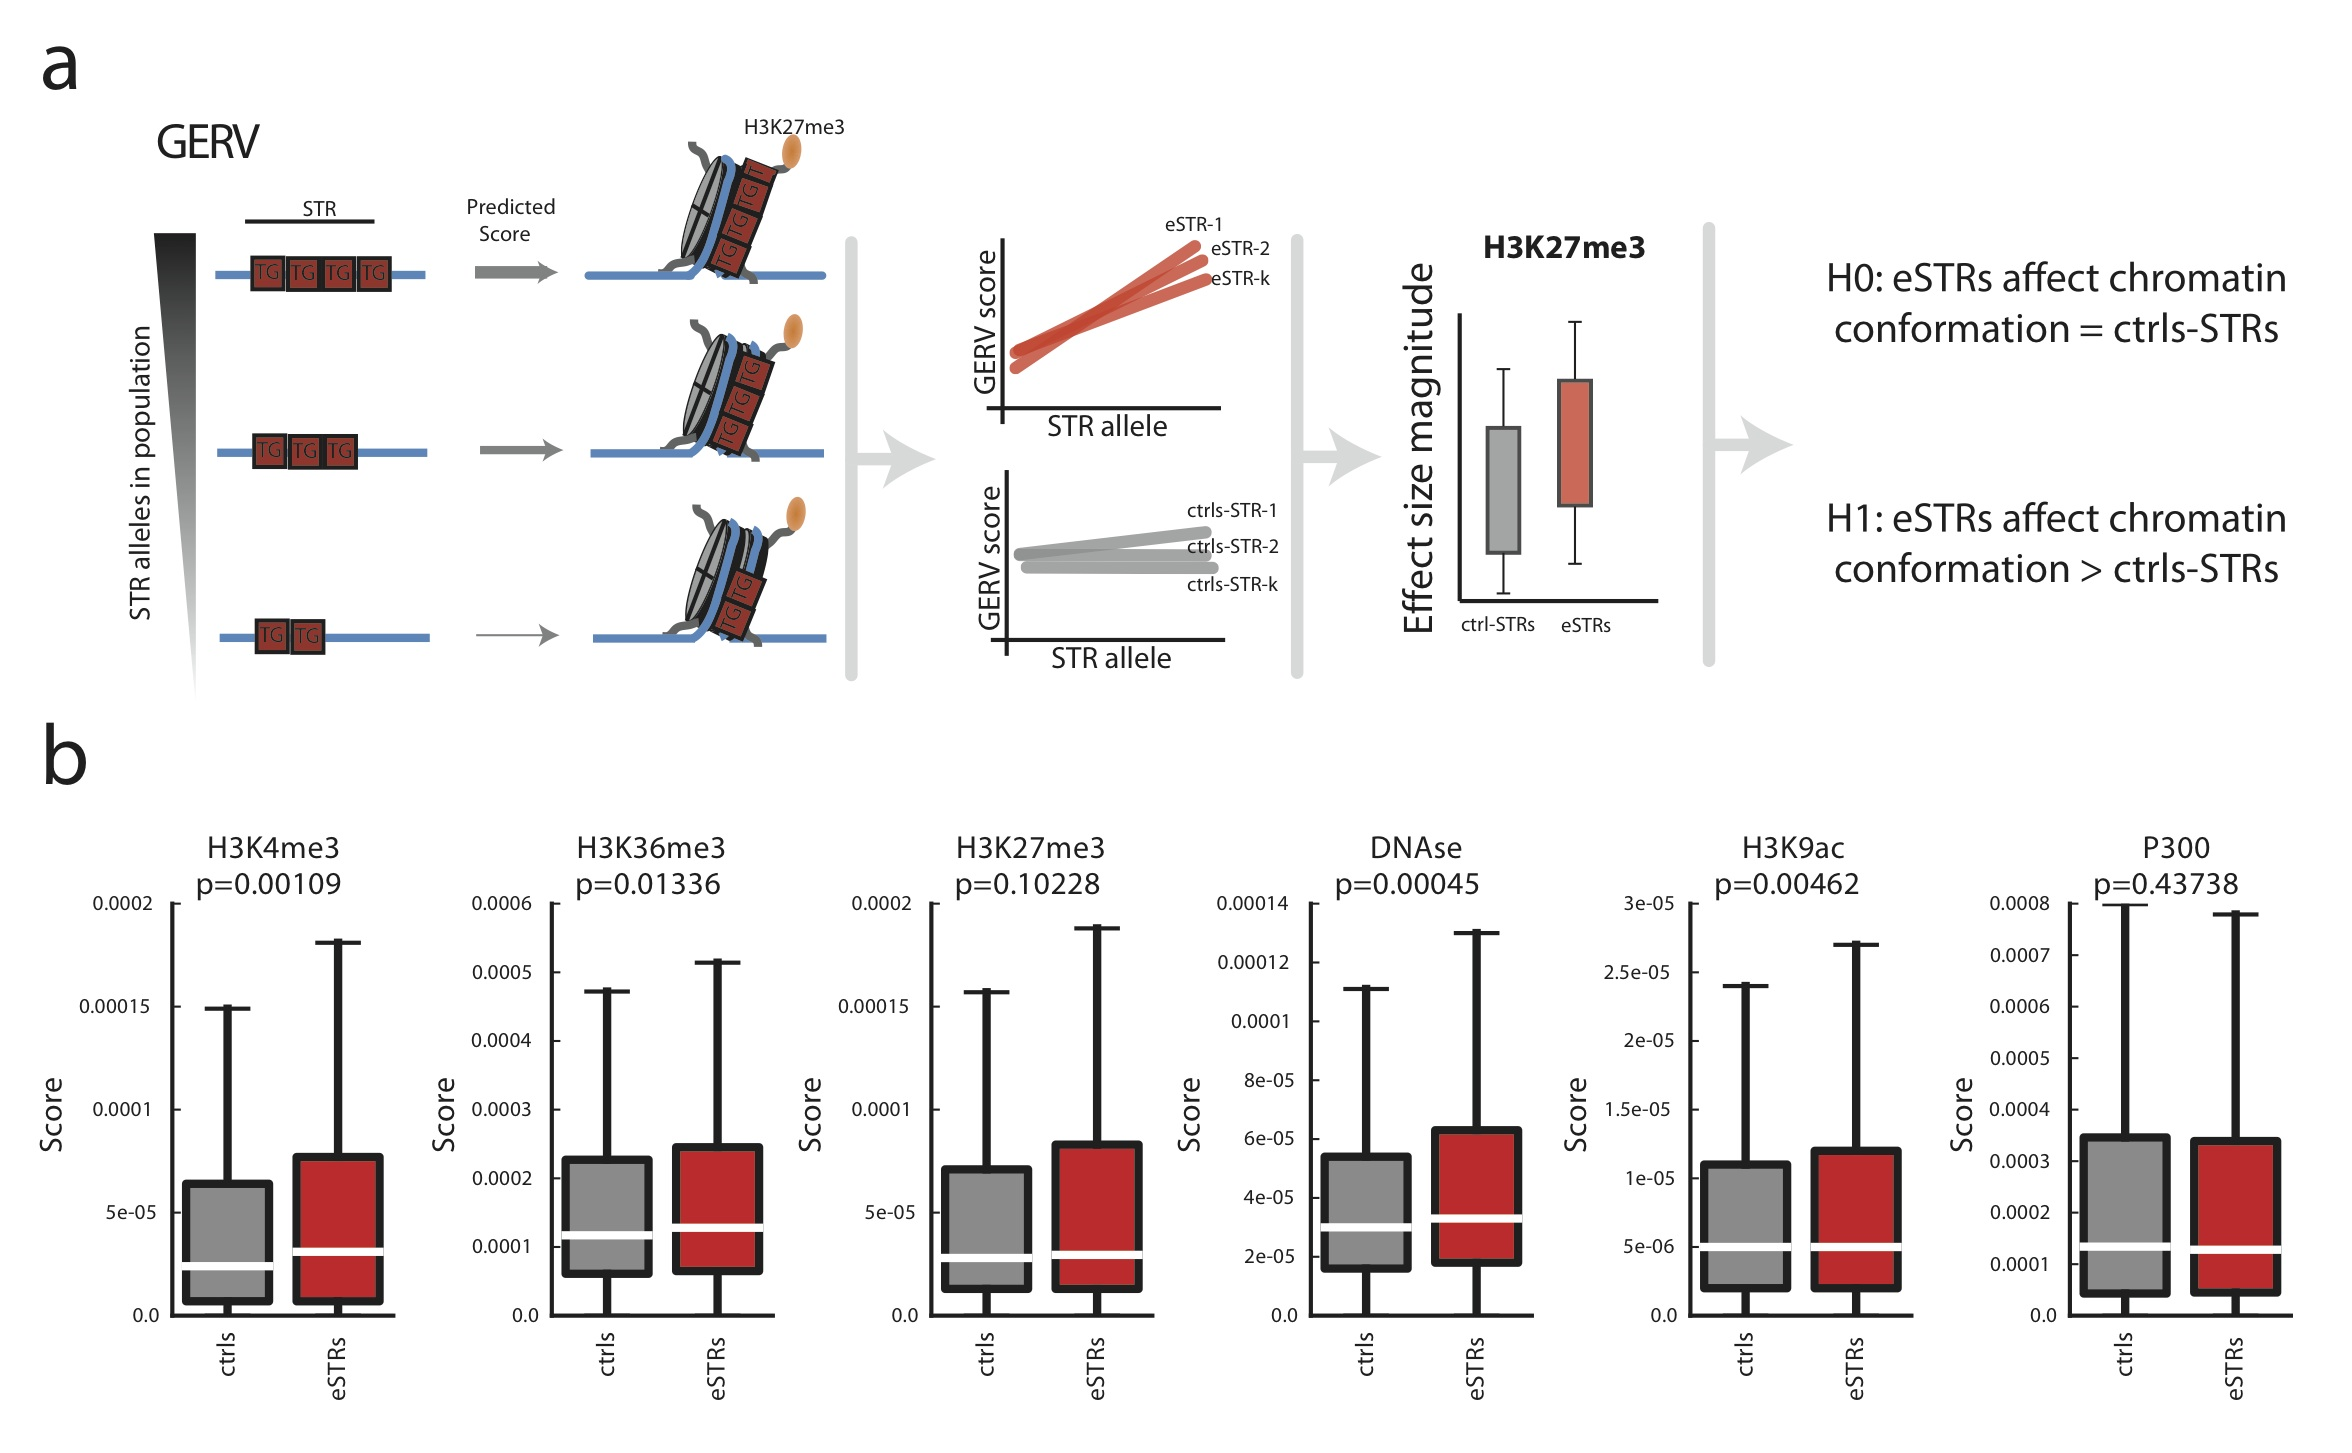
\includegraphics[width=0.7\textwidth]{Figures/Chapter4/SuppFig11.jpg}
\end{figure}
\textbf{STRs modulate epigenetic signatures}. \textbf{a}. Schematic of the application of GERV to predict histone modification signatures for different STR alleles. For each eSTR (red) and control STR (gray) we measured the magnitude of the slope between the STR allele and the GERV score and then tested whether the magnitudes were significantly different between the two sets. \textbf{b}. Comparison of the distribution of slope magnitudes for eSTRs (red) and controls (gray).

\pagebreak
\subsection{Supplementary Figure 12}
\begin{figure}[h!]
\centering
\label{fig:estrsupfig12}
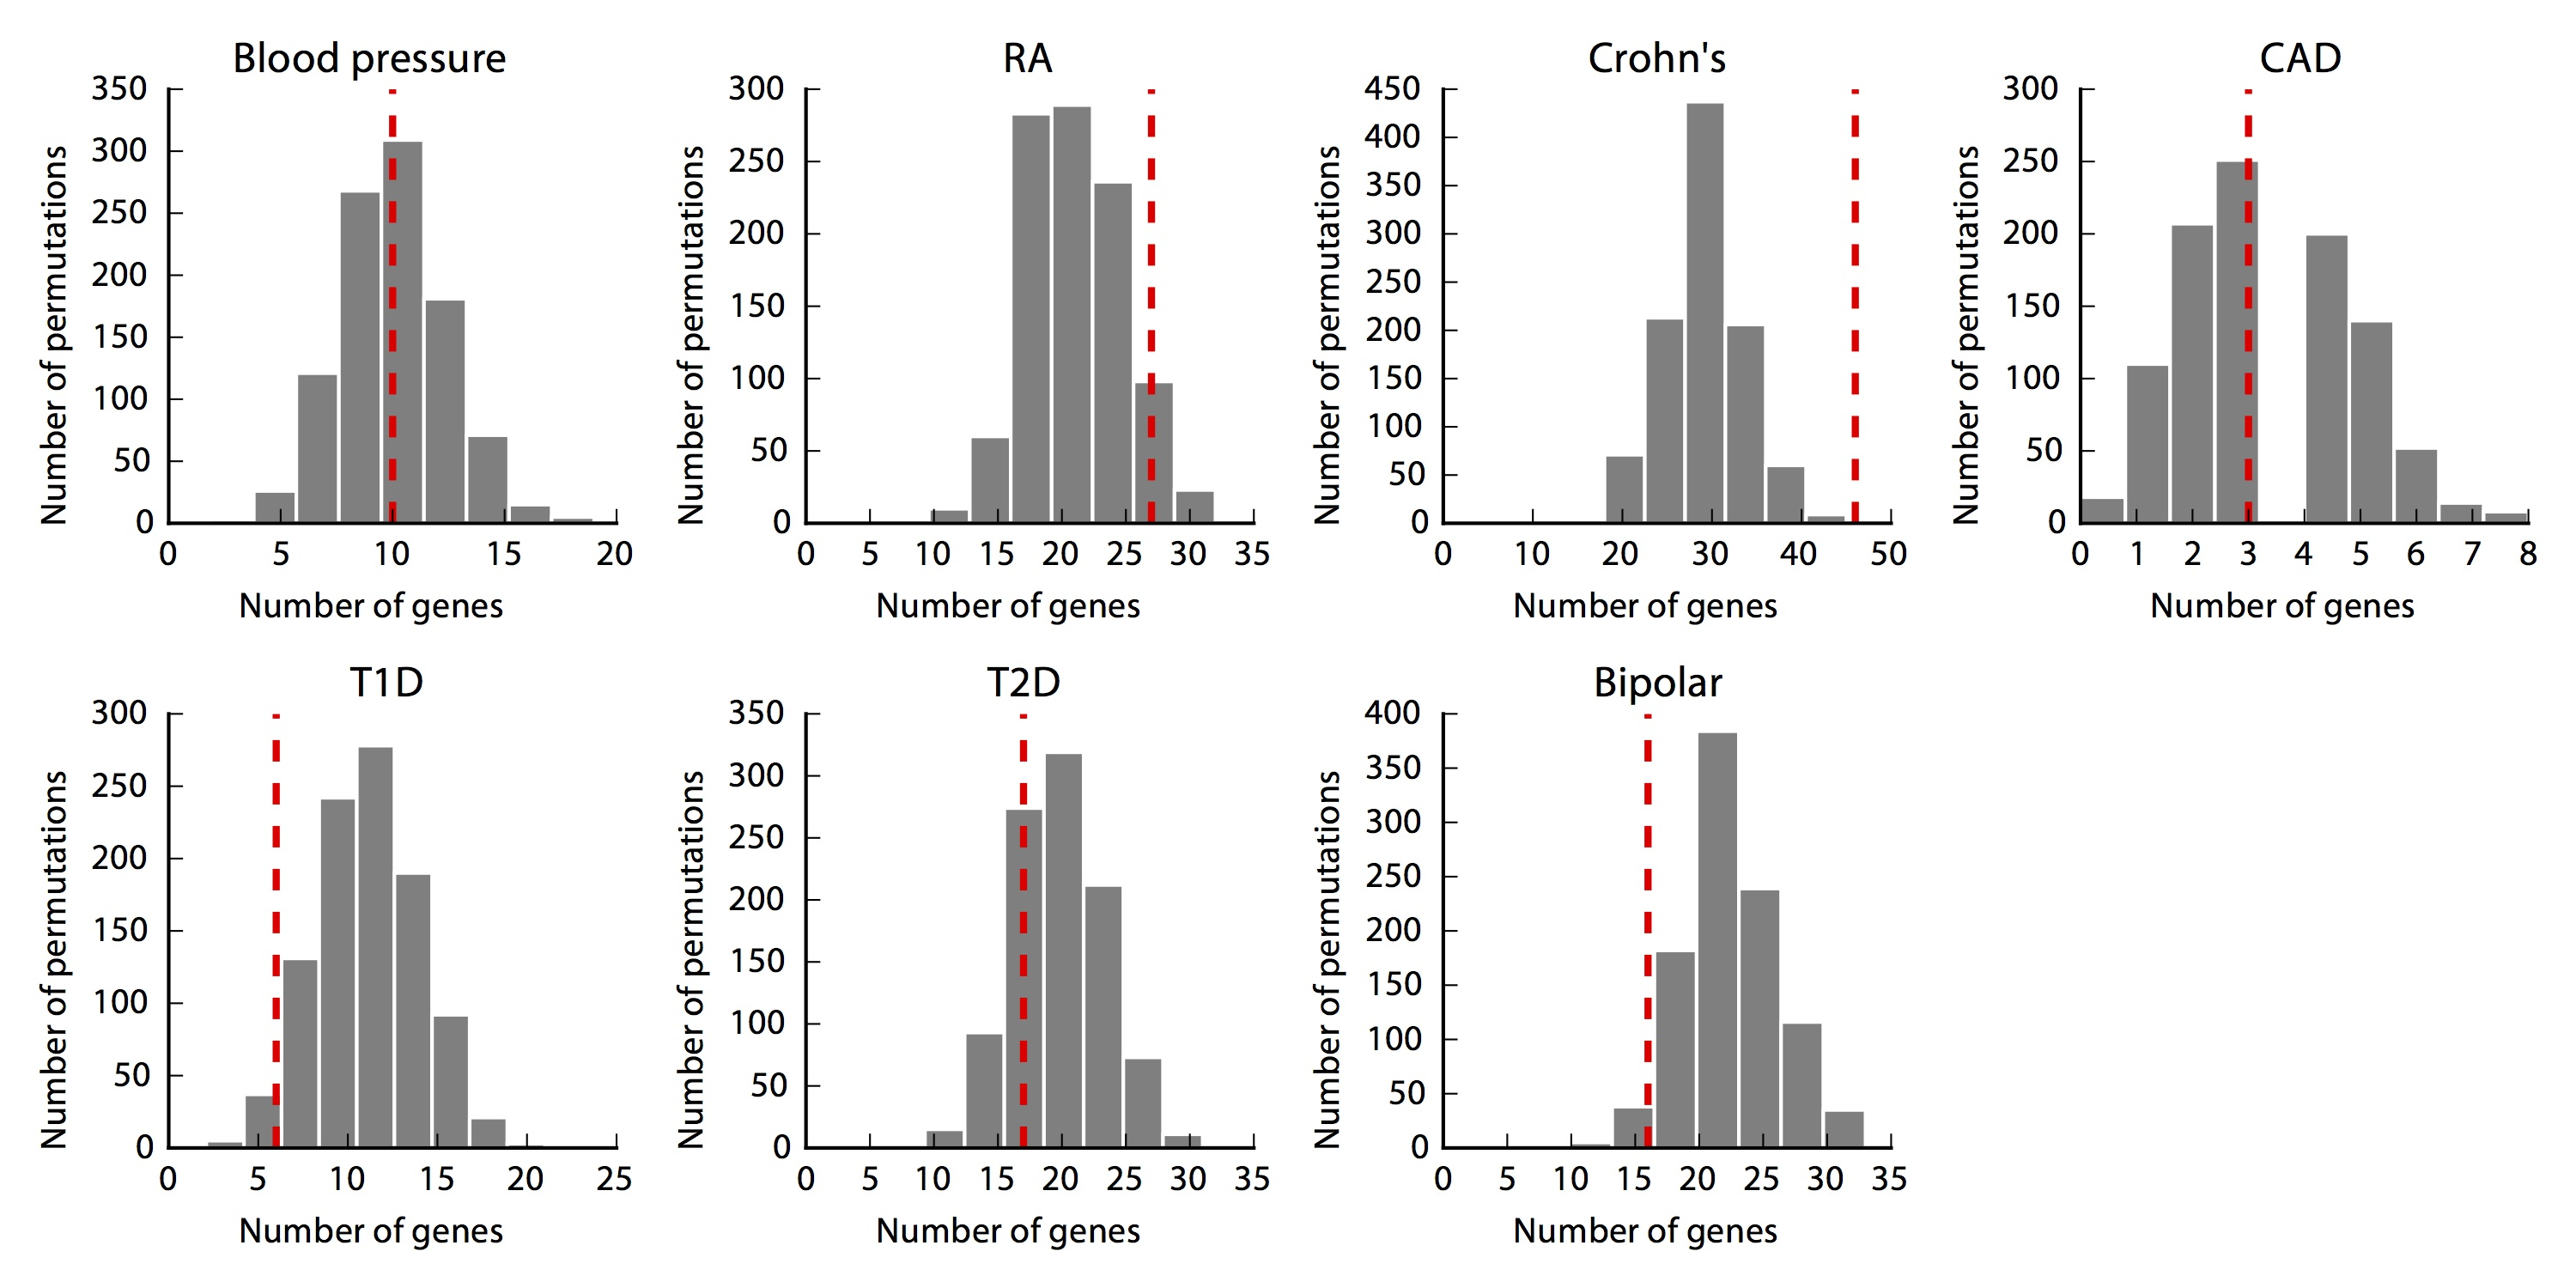
\includegraphics[width=0.7\textwidth]{Figures/Chapter4/SuppFig12.jpg}
\end{figure}
\textbf{Enrichment of eSTR genes in GWAS}. Number of eSTR genes (red dashed line) overlapping GWAS genes for each trait. Gray bars give the distribution of the number of overlapping genes from 1000 control sets of STRs matched on expression in LCLs and on \emph{cis} heritability. (RA=rheumatoid arthritis, CAD=coronary artery disease, T1D=type I diabetes, T2D=type 2 diabetes).


\pagebreak
\section{Supplementary Tables}

\subsection{Supplementary Table 1}
\label{tab:estrsuptab1}
\begin{table}[h!]
\begin{tabular}{l|l|l|l|l|l|l}
Period & Num. eSTRs & \% eSTRs & Num. all STRs & \% all STRs & Enrichment & Pval\\
\hline
2 & 951 & 50.2\% & 50,184 & 62.0\% & 0.81 & $1.0$\\
3 & 223 & 11.8\% & 7,369 & 9.1\% & 1.29 & $4.8 \times 10^{-5}$\\
4 & 516 & 27.2\% & 17,938 & 22.2\% & 1.23 & $8.2 \times 10^{-8}$\\
5 & 166 & 8.8\% & 4,466 & 5.5\% & 1.59 & $3.9 \times 10^{-9}$\\
6 & 39 & 2.1\% & 1,023 & 1.3\% & 1.63 & $2.4 \times 10^{-3}$\\
\hline
\end{tabular}
\end{table}
\textbf{Distribution of motif lengths in eSTRs vs. all STRs}. Distribution of motif lengths in all unique eSTR loci vs. all unique STR loci included in the analysis after applying quality filters. 

\pagebreak 
\subsection{Supplementary Table 2}
\label{tab:estrsuptab2}
\begin{table}[h!]
\begin{tabular}{l|l|l|l|l|l|l}
Motif & Num. eSTRs & \% eSTRs & Num. all STRs & \% all STRs & Enrichment & Pval \\
\hline
AAAAAC & 17 & 0.9\% & 217 & 0.3\% & 3.35 & $1.7 \times 10^{-5}$\\
AATC & 10 & 0.5\% & 152 & 0.2\% & 2.81 & $3.2 \times 10^{-3}$\\
AAAAC & 94 & 5.0\% & 1,822 & 2.2\% & 2.20 & $1.8 \times 10^{-12}$ \\
AAC & 95 & 5.0\% & 2,056 & 2.5\% & 1.97 & $5.0 \times 10^{-10}$\\
AAAC & 173 & 9.1\% & 3,995 & 4.9\% & 1.85 & $9.0 \times 10^{-15}$\\
AAAG & 47 & 2.4\% & 1,179 & 1.5\% & 1.70 & $3.6 \times 10^{-4}$\\
AAG & 10 & 0.5\% & 285 & 0.4\% & 1.50 & $0.13$\\
AAAAG & 15 & 0.8\% & 449 & 0.6\% & 1.43 & $0.11$\\
ATCC & 16 & 0.8\% & 488 & 0.6\% & 1.40 & $0.11$\\
ATC & 10 & 0.5\% & 392 & 0.5\% & 1.09 & $0.44$\\
AG & 128 & 6.8\% & 5,174 & 6.3\% & 1.06 & $0.27$ \\
AAAT & 198 & 10.4\% & 8,073 & 10.0\% & 1.05 & $0.25$ \\
AAAAT & 35 & 1.8\% & 1,451 & 1.8\% & 1.03 & $0.45$ \\
AATG & 16 & 0.8\% & 676 & 0.8\% & 1.01 & $0.52$\\
AAT & 74 & 3.9\% & 3,678 & 4.5\% & 0.86 & $0.92$\\
AT & 161 & 8.5\% & 8,775 & 10.8\% & 0.78 & $0.99$\\
AC & 662 & 34.9\% & 36,206& 44.7\% & 0.78 & $1.0$\\
AGAT & 16 & 0.8\% & 1,561 & 1.9\% & 0.44 & $1.0$\\
\hline
\end{tabular}
\end{table}
\textbf{Distribution of motifs in eSTRs vs. all STRs}. Distribution of motifs in all unique eSTR loci vs. all unique STR loci included in the analysis after applying quality filters. Only motifs for which there were at least 10 eSTRs are shown. Motifs were converted to canonical format as described in \cite{WillemsGymrekHighnamEtAl2014}.

\pagebreak
\subsection{Supplementary Table 3}
\label{tab:estrsuptab3}
\begin{table}[h!]
\begin{tabular}{l|l|l|l|l|l|l}
Annotation & Num. eSTRs & \% eSTRs & Num. all STRs & \% all STRs & Enrichment & Pval \\
\hline
Coding & 13 & 0.7\% & 157 & 0.2\% & 3.54 & $9.1 \times 10^{-5}$\\
5' UTR & 51 & 2.7\% & 897 & 1.1\% & 2.43 & $1.0 \times 10^{-8}$\\
Exon & 127 & 6.7\% & 2,452 & 3.0\% & 2.21 & $1.5 \times 10^{-16}$\\
3' UTR & 77 & 4.1\% & 1,569 & 1.9\% & 2.10 & $1.7 \times 10^{-9}$\\
Neargene (5') & 335 & 17.7\% & 7,357 & 9.1\% & 1.95 & $1.5 \times 10^{-32}$\\
Neargene (3') & 326 & 17.2\% & 7,399 & 9.1\% & 1.88 & $4.5 \times 10^{-29}$\\
Intron & 1,314 & 69.3\% & 52,326 & 64.6\% & 1.07 & $6.1 \times 10^{-6}$\\
Intergenic & 395 & 20.8\% & 23,373 & 28.9\% & 0.72 & $1.00$\\
\hline
\end{tabular}
\end{table}
\textbf{Distribution of genomic locations of eSTRs vs. all STRs}. Annotations were compiled using Ensembl version 71. ``Exon'' refers to both coding and non-coding exons and untranslated regions. ``Neargene'' refers to regions within 5kb of a gene. ``Intergenic'' refers to STRs not falling into any other annotation. Note some STRs may overlap multiple annotations.

\pagebreak
\subsection{Supplementary Table 4}
\label{tab:estrsuptab4}
\begin{table}[h!]
\begin{tabular}{l|l|l|l}
Element & Num. eSTRs & \% positive effects & P-val \\
\hline
All eSTRs & 2,060 & 49.5 & 0.708 \\
\hline
POL24H8 & 75 & 65.3 & 0.011 \\
DNAseI & 41 & 70.7 & 0.012 \\
5utr & 59 & 64.4 & 0.036 \\
Heterochrom/lo & 801 & 47.3 & 0.138 \\
NFIC & 51 & 60.8 & 0.161 \\
POL2 & 57 & 59.6 & 0.185 \\
WeakPromoter & 61 & 59.0 & 0.200 \\
ELF1 & 36 & 61.1 & 0.243 \\
WeakEnhancer & 151 & 45.0 & 0.255 \\
YY1 & 38 & 60.5 & 0.256 \\
TCF12 & 29 & 62.1 & 0.265 \\
WeakTxn & 496 & 52.4 & 0.302 \\
PAX5C20 & 35 & 60.0 & 0.311 \\
ATF2 & 37 & 59.5 & 0.324 \\
CREB1 & 26 & 61.5 & 0.327 \\
TxnTransition & 41 & 58.5 & 0.349 \\
RUNX3 & 91 & 54.9 & 0.402 \\
TxnElongation & 323 & 47.7 & 0.436 \\
intron & 1,434 & 49.2 & 0.579 \\
BCLAF & 48 & 54.2 & 0.665 \\
exon & 140 & 52.1 & 0.673 \\
neargene3 & 363 & 49.0 & 0.753 \\
ActivePromoter & 53 & 52.8 & 0.784 \\
Repressed & 53 & 52.8 & 0.784 \\
neargene5 & 382 & 49.2 & 0.798 \\
MTA3 & 28 & 53.6 & 0.851 \\
NFATC1 & 32 & 53.1 & 0.860 \\
FOXM1 & 38 & 52.6 & 0.871 \\
intergenic & 422 & 49.5 & 0.884 \\
3utr & 84 & 50.0 & 1.000 \\
BCL3 & 37 & 51.4 & 1.000 \\
StrongEnhancer & 79 & 50.6 & 1.000 \\
TCF3 & 37 & 48.6 & 1.000 \\
\hline
\end{tabular}
\end{table}
\textbf{Direction of effects of eSTRs}. Genomic elements were annotated using Ensembl version 71 as described in the previous table. DNAseI HS sites and transcription factor binding sites were annotated by ENCODE and were downloaded from the UCSC Table Browser for hg19.
P-values are from a two-tailed binomial test for whether the percentage of positive slopes is significantly different than 50\%.

\pagebreak
\subsection{Supplementary Table 5}
\label{tab:estrsuptab5}
\setlength\extrarowheight{2pt}
\begin{table}[h!]
\hyphenpenalty10000
\footnotesize
\begin{tabular}{|p{1.4cm}|l|p{1.2cm}|p{1.8cm}|p{1.5cm}|p{1.3cm}|p{0.8cm}|p{1.0cm}|l|l|}
\hline
\multicolumn{5}{|c|}{\textbf{Candidate gene studies}}  & \multicolumn{5}{|c|}{\textbf{Genome-wide analysis}}\\
\hline
\textbf{Reference}$^1$      & \textbf{Gene} & \textbf{STR location} & \textbf{Tissue}                               & \textbf{Direction of effect}$^2$ & \textbf{Position}$^3$   & \textbf{Effect size} &   \textbf{$\#$ of samples} & \textbf{p-value} & \textbf{eSTRs}\\
\hline
Contente, 2002    & \emph{PIG3} & 5'UTR   &  H1299 (non-small cell lung cancer)      & Inducing                & chr2: 24307212  & 0.37        & 94                & 0.00001     & Yes \\\hline
Shimajiri, 1999   & \emph{MMP9} & Promoter&  TE9 (esophageal squamous cell carcinoma)  & Inducing              & chr20: 44637413 & -0.10       & 272               & 0.06        & No\\\hline
Gebhardt, 1999    & \emph{EGFR} & Intron 1&  \emph{In vitro}								   & Repressing              & chr7: 55088254  & -0.13       & 199               & 0.07       & No\\ \hline

\end{tabular}
\end{table}
%ENSG00000146648	chr7:55088254	-0.129987993	0.070642559	0.067260955	199	AC	+	FALSE	0.115301885	FALSE
%ENSG00000115129		0.374849074	0.096655381	0.000197373	94	AGGGC	-	TRUE	0.015421827	TRUE
%ENSG00000100985	chr20	44637413	-0.102281644	0.060538891	0.0922742	272	AC	+	FALSE	0.65104834	FALSE


\textbf{Comparison of three candidate studies with STRs and their corresponding results in our genome-wide scan}
\newline
{
\footnotesize
$^1$ Full references are given in the main text.\newline
$^2$ Inducing/repressing: length increase of the STR is associated with increase/decrease of expression.\newline
$^3$ Start coordinate of the STR in hg19.\newline
}


\pagebreak
\subsection{Supplementary Table 6}
\label{tab:estrsuptab6}
\begin{table}[h!]
\begin{adjustbox}{width=1\textwidth}
\begin{tabular}{l|l|l|l}
 & $h^2_b$ & $h^2_{STR}$ & $h^2_{STR}$/$h^2_{cis}$ \\
\hline
eSTR genes (n=1,928)         &	0.1203 (0.1139-0.1259) &	0.0180 (0.0166-0.0199)	& 0.1230 (0.1106-0.1420)\\\hline
Moderate cis $h^2$ (n=6,272) &	0.0910 (0.0884-0.0938) &	0.0145 (0.0137-0.0151)	& 0.1283 (0.1222-0.1346)\\\hline
Moderate cis $h^2$, no eSTR (n=4,412) & 0.0809 (0.0791-0.0829) & 0.0136 (0.0129-0.0144) & 0.1325 (0.1262-0.1397) \\\hline
\end{tabular}
\end{adjustbox}
\end{table}
\textbf{Heritability of gene expression explained by STRs vs. common bi-allelic variants.} Values show the median and $95\%$ confidence interval of the median across all eSTR-containing genes and genes with moderate cis heritability ($\geq$5\%). $h^2_b$ denotes the variance explained by all common cis bi-allelic variants, $h^2_{STR}$ denotes the variance explained by the lead STR for each gene, and $h^2_{cis} = h^2_{STR} + h^2_b$.

\pagebreak
\subsection{Supplementary Table 7}
\label{tab:estrsuptab7}
\begin{table}[h!]
\begin{adjustbox}{width=1\textwidth}
\begin{tabular}{l|l|l|l}
 & $h^2_{b}$ & $h^2_{STR}$ & $h^2_{STR}/h^2_{cis}$ \\
\hline
 eSTR genes - (STR fixed) & 0.1203 (0.1139-0.1259) & 0.0180 (0.0166-0.0199) & 0.1230 (0.1106-0.1420) \\
 eSTR genes - (STR random) & 0.1229 (0.1159-0.1295) & 0.0200 (0.0178-0.0216) & 0.1288 (0.1179-0.1451) \\
\hline
 Moderate \emph{cis} $h^2_{cis}$ (STR fixed) & 0.0910 (0.0884-0.0938) & 0.0145 (0.0137-0.0151) & 0.1283 (0.1222-0.1346) \\
 Moderate \emph{cis} $h^2_{cis}$ (STR random) & 0.0892 (0.0865-0.0918) & 0.0143 (0.0137-0.0149) & 0.1245 (0.1184-0.1309) \\
\hline
\end{tabular}
\end{adjustbox}
\end{table}
\textbf{Heritability of gene expression explained by STRs vs. common bi-allelic variants in a random effects model.} Values show the median and 95\% confidence interval of the median across all eSTR-containing genes and genes with moderate \emph{cis} heritability ($\geq$5\%). $h^2_{b}$ denotes the variance explained by all common \emph{cis} bi-allelic markers, $h^2_{STR}$ denotes the variance explained by the lead STR for each gene, and $h^2_{cis} = h^2_{STR} + h^2_{b}$.


\pagebreak
\subsection{Supplementary Table 8}
\label{tab:estrsuptab8}
\begin{table}[h!]
\begin{tabular}{l|l|l|l|l}
Annotation & STR enrichment & STR p-value & SNP enrichment & SNP p-value \\
\hline
H3k27ac & 1.18 & 0.001 & 1.91 & $<$0.001 \\
H3k27me3 & 0.87 & 1.000 & 0.81 & 1.00 \\
H3k36me3 & 1.11 & $<$0.001 & 1.20 & $<$0.001 \\
H3k4me1 & 1.18 & $<$0.001 & 1.48 & $<$0.001 \\
H3k4me2 & 1.25 & $<$0.001 & 1.93 & $<$0.001 \\
H3k4me3 & 1.26 & $<$0.001 & 2.03 & $<$0.001 \\
H3k9ac & 1.17 & 0.009 & 2.07 & $<$0.001 \\
H3k9me3 & 0.97 & 0.804 & 1.11 & 0.001 \\
\hline
ActivePromoter & 1.00 & 0.513 & 3.41 & $<$0.001 \\
Heterochrom/lo & 0.91 & 1.000 & 0.68 & 1.000 \\
Insulator & 1.23 & 0.221 & 0.74 & 0.940 \\
PoisedPromoter & 0.56 & 0.899 & 3.14 & $<$0.001 \\
Repressed & 0.69 & 0.997 & 0.65 & 1.000 \\
StrongEnhancer & 0.98 & 0.603 & 1.93 & $<$0.001  \\
TxnElongation & 1.08 & 0.072 & 1.03 & 0.191 \\
TxnTransition & 1.07 & 0.370 & 1.09 & 0.220 \\
WeakEnhancer & 1.23 & 0.004 & 1.35 & $<$0.001  \\
WeakPromoter & 1.48 & 0.002 & 2.02 & $<$0.001  \\
WeakTxn & 1.09 & 0.012 & 1.04 & 0.057 \\
\hline
\end{tabular}
\end{table}
\textbf{Enrichment of eSNPs and eSTRs.} Overlap of eSTRs and eSNPs with each annotation were compared to the overlap of shifted eSTR and eSNP locations. We performed 1,000 rounds of shifting eSTRs and eSNPs to generate null distributions of the percent overlap. 
Enrichment values give the percent of eSTRs or eSNPs overlapping each annotation divided by the average percent overlap after shifting. P-values are empirical probabilities based on comparison to the 1,000 shifted sets of locations.

\pagebreak

\subsection{Supplementary Table 9}
\label{tab:estrsuptab9}
\footnotesize
\begin{adjustbox}{width=1\textwidth}
\csvautotabular{estr_sup_table9.csv}
\end{adjustbox}
\normalsize

\textbf{Significant associations (FDR$<$0.1) of eSTRs in the TwinsUK data.}
We considered only eSTRs for which a joint model with the lead eSNP significantly improved the explained variance of the expressed gene over a model with the lead eSNP alone. Positive effects denote STRs whose expansions are associated with increased phenotypic levels and vice versa. $R^2$ denotes the phenotypic variane explained by the STR. BP: blood pressure; CRP: C-reactive protein; MCV: Mean Corpuscular Haemoglobin. eSTR gene ids denote the genes whose expression levels were found to be associated with the eSTR. Samples denote the number of TwinsUK genomes that were genotyped and phenotyped for the specific eSTR/clinical phenotype association.  
\label{table:GWAS} 
